%  LaTeX support: latex@mdpi.com
%  In case you need support, please attach all files that are necessary for compiling as well as the log file, and specify the details of your LaTeX setup (which operating system and LaTeX version / tools you are using).

%=================================================================
\documentclass[Dance Data
Project,article,submit,moreauthors,pdftex]{mdpi}

% If you would like to post an early version of this manuscript as a preprint, you may use preprint as the journal and change 'submit' to 'accept'. The document class line would be, e.g., \documentclass[preprints,article,accept,moreauthors,pdftex]{mdpi}. This is especially recommended for submission to arXiv, where line numbers should be removed before posting. For preprints.org, the editorial staff will make this change immediately prior to posting.

%% Some pieces required from the pandoc template
\setlist[itemize]{leftmargin=*,labelsep=5.8mm}
\setlist[enumerate]{leftmargin=*,labelsep=4.9mm}


%--------------------
% Class Options:
%--------------------
%----------
% journal
%----------
% Choose between the following MDPI journals:
% acoustics, actuators, addictions, admsci, aerospace, agriculture, agriengineering, agronomy, algorithms, animals, antibiotics, antibodies, antioxidants, applsci, arts, asc, asi, atmosphere, atoms, axioms, batteries, bdcc, behavsci , beverages, bioengineering, biology, biomedicines, biomimetics, biomolecules, biosensors, brainsci , buildings, cancers, carbon , catalysts, cells, ceramics, challenges, chemengineering, chemistry, chemosensors, children, cleantechnol, climate, clockssleep, cmd, coatings, colloids, computation, computers, condensedmatter, cosmetics, cryptography, crystals, dairy, data, dentistry, designs , diagnostics, diseases, diversity, drones, econometrics, economies, education, electrochem, electronics, energies, entropy, environments, epigenomes, est, fermentation, fibers, fire, fishes, fluids, foods, forecasting, forests, fractalfract, futureinternet, futurephys, galaxies, games, gastrointestdisord, gels, genealogy, genes, geohazards, geosciences, geriatrics, hazardousmatters, healthcare, heritage, highthroughput, horticulturae, humanities, hydrology, ijerph, ijfs, ijgi, ijms, ijns, ijtpp, informatics, information, infrastructures, inorganics, insects, instruments, inventions, iot, j, jcdd, jcm, jcp, jcs, jdb, jfb, jfmk, jimaging, jintelligence, jlpea, jmmp, jmse, jnt, jof, joitmc, jpm, jrfm, jsan, land, languages, laws, life, literature, logistics, lubricants, machines, magnetochemistry, make, marinedrugs, materials, mathematics, mca, medicina, medicines, medsci, membranes, metabolites, metals, microarrays, micromachines, microorganisms, minerals, modelling, molbank, molecules, mps, mti, nanomaterials, ncrna, neuroglia, nitrogen, notspecified, nutrients, ohbm, particles, pathogens, pharmaceuticals, pharmaceutics, pharmacy, philosophies, photonics, physics, plants, plasma, polymers, polysaccharides, preprints , proceedings, processes, proteomes, psych, publications, quantumrep, quaternary, qubs, reactions, recycling, religions, remotesensing, reports, resources, risks, robotics, safety, sci, scipharm, sensors, separations, sexes, signals, sinusitis, smartcities, sna, societies, socsci, soilsystems, sports, standards, stats, surfaces, surgeries, sustainability, symmetry, systems, technologies, test, toxics, toxins, tropicalmed, universe, urbansci, vaccines, vehicles, vetsci, vibration, viruses, vision, water, wem, wevj

%---------
% article
%---------
% The default type of manuscript is "article", but can be replaced by:
% abstract, addendum, article, benchmark, book, bookreview, briefreport, casereport, changes, comment, commentary, communication, conceptpaper, conferenceproceedings, correction, conferencereport, expressionofconcern, extendedabstract, meetingreport, creative, datadescriptor, discussion, editorial, essay, erratum, hypothesis, interestingimages, letter, meetingreport, newbookreceived, obituary, opinion, projectreport, reply, retraction, review, perspective, protocol, shortnote, supfile, technicalnote, viewpoint
% supfile = supplementary materials

%----------
% submit
%----------
% The class option "submit" will be changed to "accept" by the Editorial Office when the paper is accepted. This will only make changes to the frontpage (e.g., the logo of the journal will get visible), the headings, and the copyright information. Also, line numbering will be removed. Journal info and pagination for accepted papers will also be assigned by the Editorial Office.

%------------------
% moreauthors
%------------------
% If there is only one author the class option oneauthor should be used. Otherwise use the class option moreauthors.

%---------
% pdftex
%---------
% The option pdftex is for use with pdfLaTeX. If eps figures are used, remove the option pdftex and use LaTeX and dvi2pdf.

%=================================================================
\firstpage{1}
\makeatletter
\setcounter{page}{\@firstpage}
\makeatother
\pubvolume{xx}
\issuenum{1}
\articlenumber{5}
\pubyear{2019}
\copyrightyear{2019}
%\externaleditor{Academic Editor: name}
\history{Received: date; Accepted: date; Published: date}
\updates{yes} % If there is an update available, un-comment this line

%% MDPI internal command: uncomment if new journal that already uses continuous page numbers
%\continuouspages{yes}

%------------------------------------------------------------------
% The following line should be uncommented if the LaTeX file is uploaded to arXiv.org
%\pdfoutput=1

%=================================================================
% Add packages and commands here. The following packages are loaded in our class file: fontenc, calc, indentfirst, fancyhdr, graphicx, lastpage, ifthen, lineno, float, amsmath, setspace, enumitem, mathpazo, booktabs, titlesec, etoolbox, amsthm, hyphenat, natbib, hyperref, footmisc, geometry, caption, url, mdframed, tabto, soul, multirow, microtype, tikz

%=================================================================
%% Please use the following mathematics environments: Theorem, Lemma, Corollary, Proposition, Characterization, Property, Problem, Example, ExamplesandDefinitions, Hypothesis, Remark, Definition
%% For proofs, please use the proof environment (the amsthm package is loaded by the MDPI class).

%=================================================================
% Full title of the paper (Capitalized)
\Title{Analysis of Dance Data Company Endowments, Assets, and Labor in
the United States}

% Authors, for the paper (add full first names)
\Author{Rose
Evard$^{1}$\href{https://orcid.org/0000-0003-3293-2315}{\orcidicon}, Ruth
Button$^{1}$, Zhen
Nie$^{1}$\href{https://orcid.org/0009-0009-3690-4953}{\orcidicon}, Quinn
White$^{1}$\href{https://orcid.org/0000-0001-5399-0237}{\orcidicon}}

% Authors, for metadata in PDF
\AuthorNames{Rose Evard, Ruth Button, Zhen Nie, Quinn White}

% Affiliations / Addresses (Add [1] after \address if there is only one affiliation.)
\address{%
$^{1}$ \quad Smith College Statistical \& Data Sciences Department 1
Chapin Way, Northampton, MA, 01063; \\
}
% Contact information of the corresponding author
\corres{Correspondence: \href{mailto:andrew.hoekstra@dancedataproject.com}{\nolinkurl{andrew.hoekstra@dancedataproject.com}}}

% Current address and/or shared authorship








% The commands \thirdnote{} till \eighthnote{} are available for further notes

% Simple summary

% Abstract (Do not insert blank lines, i.e. \\)

% Keywords
\keyword{Endowment; Non-Profit; Volunteer Labor; Dance.}

% The fields PACS, MSC, and JEL may be left empty or commented out if not applicable
%\PACS{J0101}
%\MSC{}
%\JEL{}

%%%%%%%%%%%%%%%%%%%%%%%%%%%%%%%%%%%%%%%%%%
% Only for the journal Diversity
%\LSID{\url{http://}}

%%%%%%%%%%%%%%%%%%%%%%%%%%%%%%%%%%%%%%%%%%
% Only for the journal Applied Sciences:
%\featuredapplication{Authors are encouraged to provide a concise description of the specific application or a potential application of the work. This section is not mandatory.}
%%%%%%%%%%%%%%%%%%%%%%%%%%%%%%%%%%%%%%%%%%

%%%%%%%%%%%%%%%%%%%%%%%%%%%%%%%%%%%%%%%%%%
% Only for the journal Data:
%\dataset{DOI number or link to the deposited data set in cases where the data set is published or set to be published separately. If the data set is submitted and will be published as a supplement to this paper in the journal Data, this field will be filled by the editors of the journal. In this case, please make sure to submit the data set as a supplement when entering your manuscript into our manuscript editorial system.}

%\datasetlicense{license under which the data set is made available (CC0, CC-BY, CC-BY-SA, CC-BY-NC, etc.)}

%%%%%%%%%%%%%%%%%%%%%%%%%%%%%%%%%%%%%%%%%%
% Only for the journal Toxins
%\keycontribution{The breakthroughs or highlights of the manuscript. Authors can write one or two sentences to describe the most important part of the paper.}

%\setcounter{secnumdepth}{4}
%%%%%%%%%%%%%%%%%%%%%%%%%%%%%%%%%%%%%%%%%%


% tightlist command for lists without linebreak
\providecommand{\tightlist}{%
  \setlength{\itemsep}{0pt}\setlength{\parskip}{0pt}}

% From pandoc table feature
\usepackage{longtable,booktabs,array}
\usepackage{calc} % for calculating minipage widths
% Correct order of tables after \paragraph or \subparagraph
\usepackage{etoolbox}
\makeatletter
\patchcmd\longtable{\par}{\if@noskipsec\mbox{}\fi\par}{}{}
\makeatother
% Allow footnotes in longtable head/foot
\IfFileExists{footnotehyper.sty}{\usepackage{footnotehyper}}{\usepackage{footnote}}
\makesavenoteenv{longtable}


\usepackage{caption}
\captionsetup[figure]{font=scriptsize}
\usepackage{subfig}
\usepackage{booktabs}
\usepackage{longtable}
\usepackage{array}
\usepackage{multirow}
\usepackage{wrapfig}
\usepackage{float}
\usepackage{colortbl}
\usepackage{pdflscape}
\usepackage{tabu}
\usepackage{threeparttable}
\usepackage{threeparttablex}
\usepackage[normalem]{ulem}
\usepackage{makecell}
\usepackage{xcolor}

\begin{document}


%%%%%%%%%%%%%%%%%%%%%%%%%%%%%%%%%%%%%%%%%%

\hypertarget{executive-summary}{%
\section{Executive Summary:}\label{executive-summary}}

In an effort to advance equity in dance, this report examines existing
financial structures and incentives that shape dance companies' fiscal
viability. This report was produced in conjunction with a team of
students from the Smith College Statistical \& Data Sciences Capstone,
hereafter referred to as the capstone team.

The capstone team reviewed publicly-available tax forms from 169 dance
companies in the United States for information on their endowments over
time, use of labor, compensation, investments, and other assets. When
comparing against the S\&P 500 as a measure of the state of the stock
market, the capstone team found that the trends in companies' endowments
closely follow those in the stock market in general, but some companies
do
\hyperref[fig:annual-growth-endowment]{diverge from these general trends}.
Notably, some companies do not invest their endowments for most years on
file (e.g., Dance Theatre of Harlem, Eugene Ballet, or the American
Repertory Ballet).

Form 990 requires companies to estimate the company's total number of
volunteers that did any amount of volunteer work during the fiscal year.
Unpaid labor is especially important to investigate because the Bureau
of Labor Statistics indicates that 76.6\% of the workforce is female,
and the wage gap is especially apparent in dance
\citep{jikar_gender_2022}. In terms of labor usage, the West region uses
the most combined employee and volunteer labor, but the South region has
the highest percentage of companies with more volunteers than employees.
The Team also determined that the fraction of compensation going to top
executives is generally consistent from 2014 - 2020, with a median near
10\%. There is more variability in the fraction paid to top executives
for smaller companies. These trends in executive compensation will be
important to track as filings are released for the pandemic years.

The value of this research is in its ability to impact future data
advocacy in regard to dance companies in the United States. As well,
this project provides a framework for the analysis of Form 990 data,
including publicly available code, to bring more transparency to the
financial side of the dance industry. Of note, a major limitation of
this report is that it relies on publicly-available, online tax
documents which may contain errors or false reporting. Additionally, the
IRS is currently behind in posting recent tax documents as well as
updated amendments, so few filings are available for the fiscal year
2021, and no filings beyond 2021 are available. Dance Data Project® does
not seek to make inferences based on the data presented here; rather,
Dance Data Project (DDP®) records and reports the data as it is reported
on the IRS website.

\hypertarget{introduction}{%
\section{Introduction}\label{introduction}}

\hypertarget{inequality-in-the-arts}{%
\subsection{Inequality in the Arts}\label{inequality-in-the-arts}}

Discrepancies in how nonprofits report financial data can impact those
already at a social and economic disadvantage, such as women and girls
\citep{fuchs_where_2021}. The study of women and gender has consistently
drawn focus to the inequitable distribution of wealth between men and
women. One of the most heavily researched phenomena regarding wealth
inequality is the wage gap between men and women that persists even when
they have the same education, experience, skills, and job titles
\citep{jikar_gender_2022}. Contrary to the popular opinion that the
gender wage gap is narrowing, Weichselbaumer \& Winter-Ebmer
\citep{weichselbaumer_meta-analysis_2005} demonstrated that financial
returns in relation to skills and education are increasingly higher for
men than for women. Even less research has been done on the wage gap for
transgender or non-binary individuals. Additionally, compounding factors
such as lack of corporate oversight and socially-imposed gender roles
further entrench the gender pay gap into everyday life
\citep{noauthor_handbook_2013}. Further understanding the wage gap in
female-dominated fields, such as in dance, can inform future solutions
to lessen the inequitable distribution of wealth between men and women.

The wage gap has long been exacerbated by disproportionate pay in the
arts, and especially dance, in part because the vast majority of
entry-level dancers are women and girls \citep{jikar_gender_2022}.
Additionally, unpaid labor in dance is much more commonplace than in
other industries \citep{noauthor_handbook_2013}. Because dance is a
performing art, many companies that employ dancers are entitled to
government subsidies and tax breaks; however, there are no current
regulations to ensure that this governmental assistance is used to
lessen unpaid and underpaid labor by dancers \citep{fuchs_where_2021}.
Unrestricted financial assistance may worsen existing inequalities in
the field of dance by enabling company owners and executives to profit
while retaining unpaid and underpaid labor, so further understanding how
this assistance is used is essential in combating the problem.

\hypertarget{the-dance-data-project}{%
\subsection{The Dance Data Project}\label{the-dance-data-project}}

The capstone team completed this project in collaboration with our
project sponsor, the Dance Data Project (also known as DDP®). The Dance
Data Project is a non-profit organization dedicated to equality in the
arts. Founded in 2015 by philanthropist Elizabeth Yntema, DDP® uses data
and research to promote transparency, accountability, and action toward
gender equality in dance.

DDP® collects, analyzes, and presents data to outline the lack of
leadership opportunities for female directors, choreographers,
composers, set, costume, lighting designers, and back-of-house positions
in dance. The organization seeks to create a world where all dancers,
regardless of gender, race, ethnicity, or socioeconomic status, have
equal access to opportunities and resources in the dance world. The
organization also advocates for removing barriers to female employment
and advancement in this industry, such as lack of parental and elder
leave, daycare system, and protocol for sexual harassment by presenting
their findings on television news such as
\href{https://www.youtube.com/watch?t=2532\&v=eWL_r5Gq2Vk\&feature=youtu.be}{NBC/NOW}
and publishing articles in magazines such as
\href{https://www.nytimes.com/2022/01/21/arts/dance/gender-gap-ballet.html}{\emph{New
York Times}},
\href{https://www.forbes.com/sites/kimelsesser/2019/09/12/a-gender-gap-in-ballet-seriously/?sh=7b9f066d2be6}{\emph{Forbes}},
\href{https://fortune.com/2022/01/25/board-diversity-cant-find-women-pipeline-problem/}{\emph{Fortune}},
and
\href{https://www.dancemagazine.com/with-its-free-raising-the-barre-curriculum-dance-data-project-aims-to-get-more-women-into-leadership-positions/}{Dance
Magazine}. Through its data-driven research, advocacy, and education
efforts, DDP® works to create a more equitable and inclusive dance
community where all individuals have the opportunity to pursue their
passion for dance.

\hypertarget{scope}{%
\subsection{Scope}\label{scope}}

As a matter of transparency and public accountability, tax documents
filed by nonprofit corporations in the United States have always
theoretically been available to the public, but it wasn't until the
development of electronic tax filing systems through the IRS that these
tax documents became easily accessible for analysis. Online tax filing
systems have been available since the late 1990s, but the
\href{https://www.congress.gov/bill/116th-congress/house-bill/3151}{2019
Taxpayer First Act} required all nonprofits to electronically file their
tax returns \citep{ely_research_2023}. This legislation changed the
landscape for public accessibility of the financial information of
nonprofits as well as presented critical research opportunities for data
activism. Incorrect reporting, inequitable wealth distribution, and tax
fraud by nonprofit organizations have always happened, but mandatory
online reporting allows data analysts to identify suspected cases and
draw attention to them \citep{ely_research_2023}.

\hypertarget{the-dance-economy-irs-form-990s}{%
\subsection{The Dance Economy \& IRS Form
990s}\label{the-dance-economy-irs-form-990s}}

In the United States, nonprofit organizations file either a Form 900 or
a Form 990 EZ with the IRS each year. These documents include but are
not limited to information on the organization's geographic location,
number of employees and volunteers, operating costs, income,
compensation, and net assets. Additionally, some nonprofits are required
to fill out Schedule D forms alongside their 990 filings if they have
certain additional assets (i.e.~endowment funds, real estate, investment
income). Each organization reports these values for their own fiscal
years. It is important to understand that companies have different dates
for their fiscal years, so one company may report a fiscal year ending
in February and another may report their fiscal year ending in
September. This causes significant variability when analyzing 990 forms
from different companies \citep{ely_research_2023}.

Form 990 data is more accessible than ever now and the government has
required nonprofit organizations to electronically file them. Yet, much
of the public does not understand the terms on publicly available tax
forms, nor does the average person possess the skills to readily analyze
hundreds of tax forms every year \citep{lamothe_examining_2023}. Thus,
data scientists can play a very important role in analyzing these forms
filed by dance companies and presenting findings to the public. Further
elucidating the financial practices of nonprofit organizations 1) in the
field of dance, 2) in pandemic-related economic shifts and 3) through
geographical analysis can help inform proper solutions to a wide range
of issues, including difference in cost of living and performance season
in different regions and the different features in regional gender pay
gap in dance.

\hypertarget{current-study}{%
\subsection{Current Study}\label{current-study}}

This project provides a preliminary analysis of publicly available
financial information on dance companies in the United States. Results
were collected and shared with Dance Data Project for any publications
or future analyses that they perform. Because little previously publicly
available research has been published regarding the financial practices
of dance companies in the United States, our exploratory approach
examined broad research areas regarding how dance companies manage
endowments, employment, and properties.

The bulk of this report consists of examining how companies' financial
resources (particularly endowments) behave over time, in comparison to
one another, and in comparison to the S\&P 500. The use of volunteer
labor alongside the use of paid employment labor and how geographical
location impacts the use of each type of labor is also investigated.

The data source for this project is a collection of IRS Form 990 and IRS
Form 990 EZ from dance companies in the United States; as a result, the
dataset utilized for this project only contained IRS Form 990s which
have been accepted, processed, and published online by the IRS. These
publicly available tax documents are required annual filings for
nonprofits\footnote{Most major dance companies are nonprofits.} and
include information such as the number of employees and volunteers,
compensation to employees, geographical location, and annual revenue. As
part of Form 990s, companies with certain financial assets must report
Schedule D forms, which contain data on endowment funds as well as
building values and other assets. The analysis is primarily presented
based on Schedule D of Form 990. This analysis seeks to capture trends
in how these companies have managed their assets and endowments,
primarily in the time span of 2014 to 2020, with the goal of bringing
transparency to the financial side of the dance industry.

\hypertarget{ethics-statement}{%
\section{Ethics Statement}\label{ethics-statement}}

This project included signing a non-disclosure agreement with Dance Data
Project in which each group member agreed to keep specific collections
of data produced by DDP® confidential.\\
In these analyses, the team assumed the values from the most recent
filings were correct. Amended filings were used when available; however,
it is possible that companies have made amendments that have not yet
been released by the IRS. As of January 2023, written returns are no
longer accepted. The social harm that could occur from this assumption
is that dance companies who accidentally misreport their tax documents
may be identified in the following analyses as violating ethical or
financial norms. In order to prevent this, the team and DDP®
collaborated to reach out to companies to ask for clarification of the
below findings before potentially publishing their name.

Finally, all of the capstone team have training in data science. Because
none of the Team members have a background in dance, the Team members
cannot provide personal expertise in analyzing this data. Additionally,
the capstone team all identifies as female and has limited racial
diversity with no input from the Black community. The standpoints of
dancers, men, and people of diverse backgrounds in data analyses may
offer a more comprehensive understanding of the context behind the
utilized dataset. In order to reduce bias (although it was not possible
to change the team's social identities), the capstone team spoke with
the Dance Data Project about how to approach this data that may impact
other social groups.

\hypertarget{detailed-methodology}{%
\section{Detailed Methodology}\label{detailed-methodology}}

\hypertarget{data-acquisition}{%
\subsection{Data Acquisition}\label{data-acquisition}}

Data files were gathered by Andrew Hoekstra, data consultant from DDP®,
prior to February 8th, 2022 from publicly available IRS APIs. Form 990s
were downloaded as XMLs. The sample contained 169 US dance companies in
total, with Form 990s submitted between 2015 and 2022, thus representing
fiscal years 2014 through 2021; however, as more recent filings are
currently unavailable through the IRS, not all companies who filed in
2022 are represented in fiscal year 2021 within this analysis. For
Schedule D in particular, companies are required to report endowment
totals up to 4 fiscal years prior, thus the utilized endowment data
spans 2010 to 2021.

\hypertarget{initial-wrangling-filtering}{%
\subsection{Initial Wrangling \&
Filtering}\label{initial-wrangling-filtering}}

Form 990 can be completed in three different formats: Form 990, Form
900-EZ, and Form 990-T. All Form 990-Ts were excluded because these
forms do not contain relevant information on variables considered in the
following analyses. Additionally, when a company amended a filing, and
hence had multiple filings corresponding to a single fiscal year, the
amended filing was used.

\hypertarget{quality-assurance}{%
\subsection{Quality Assurance}\label{quality-assurance}}

Because in a single filing, a company reports years for several
endowment variables not only for the current year but for the prior
year, two years back, three years back, and four years back, filings
across years can be cross-referenced to ensure they are concordant.

For example, when a company reports in their 2020 filing the beginning
of year endowment balance for years 2016 through 2020, the value they
reported for 2016 in the 2020 filing (in the four years back column) can
be cross-referenced with what they reported in 2016 (in the current year
column) to ensure reporting consistency. Reporting was highly consistent
across the companies considered; however, there were some notable
discrepancies, particularly in earlier years. When these discrepancies
were identified, the capstone team reached out to the companies to
clarify which values were correct (Table \ref{table:discrep}). The team
received prompt responses from BalletMet and Pittsburgh Ballet, who
confirmed the more recently reported values were correct.

Because discrepancies were typically in earlier years, and our
communications with the companies who did respond noted their most
recently reported values were correct, in our analyses the most recent
data available was used. For example, values for 2016-2020 were taken
from the 2020 filing instead of taking the current year's values for the
filing from each year separately.

Another result of this approach is that it is possible to look back
through the fiscal year 2010 in some cases since although filings only
go back to 2014, each filing has data going back four years.

\hypertarget{asfb}{%
\section{\texorpdfstring{\emph{Nota Bene} regarding Aspen Santa Fe
Ballet}{Nota Bene regarding Aspen Santa Fe Ballet}}\label{asfb}}

\label{sec:asfb}

There are a couple of important notes to make about Aspen Santa Fe as we
interpret the figures in this report.

For one, Aspen Santa Fe transferred a large proportion of its endowment
to the entity
\href{https://projects.propublica.org/nonprofits/organizations/821009713}{Aspen
Santa Fe Ballet Endowment Inc} (EIN 821009713) in 2018. This must be
considered when interpreting the changes in endowment over time. Aspen
Santa Fe Ballet shuttered its professional company in March 2020.

According to their executive director and accountant, there were issues
with Aspen Santa Fe Ballet's filing for the fiscal year 2020, which have
been amended. However, this amended filing has not yet been released by
the IRS, and thus it cannot be included in this analysis.

\begin{table}[H]

\caption{\label{tab:unnamed-chunk-1}\label{table:discrep}Companies Reached Out to Regarding Discrepancies}
\centering
\begin{tabular}[t]{l>{\raggedright\arraybackslash}p{35em}}
\toprule
Company & Discrepancy\\
\midrule
Aspen Santa Fe & The current year value for other expenditures for fiscal year 2018 is \$6,906,449, but in 2019 the prior year value for other expenditures is \$6,356,449 and, in accordance with the 2019 report, in 2020 the two years back value is \$6,356,449. DDP has corresponded with Aspen Santa Fe Ballet regarding this discrepancy; however, the amended return is not available through the IRS at this point in time.\\
\addlinespace
BalletMet & In 2015, the current year beginning of year balance is reported as \$262,509, but then in 2016, the prior year beginning year balance is said to be \$235,225; future year filings are in accordance with the \$235,225 value.\\
\addlinespace
Ballet Arizona & In the 2016 and 2017 filings, the beginning of year balance corresponding to fiscal years 2016 and 2017 was reported as \$101,399. However, in the 2018 filing, the value for 2016 was reported to be \$601,399, and the value corresponding to 2017 was reported as \$4,126,424.\\
\addlinespace
The Alabama Ballet & In the filings for fiscal years 2016, 2017, and 2018,  the beginning and end of year balances are marked as \$250,000 for all included years. However, in 2019, the value reported for the prior year (2018)  is \$477,040, and in the filing for the fiscal year 2020, the values are not concordant with the \$250,000 value.\\
\addlinespace
Fort Wayne Ballet & In the 2017 filing, the beginning-of-year balance is \$1,264,981. However, in the 2018 filing, the beginning of year balance for the prior year is reported as \$1,291,109 (second image below, and then the 2019 and 2020 filings both report the value corresponding to 2017 as \$1,413,780. There are similar discrepancies for the end of year balances.\\
\addlinespace
Joffrey Ballet & In the filing for the 2015 fiscal year, the value corresponding to 2015 is \$1,443,297, and the value corresponding to the 2014 filing is recorded as \$170,360.  However, in 2016, the value corresponding to 2015 is reported as \$1,136,139, and the value for 2014 is reported as \$35,600. Additionally, the reported contributions amount (under Part V: endowment funds)  for the filing on fiscal year 2016 is \$236,579, but in 2017 the contributions amount reported for the prior year (2016) is \$278,281; the value of \$278,281 is reported in following years.\\
\addlinespace
The San Francisco Ballet & In San the tax filings corresponding to fiscal year 2015, the beginning of year balance for 2013, 2014, and 2015 are reported as \$174.  These values are in accordance with the fiscal year 2016 filing, and the beginning of year balance for 2016 is also reported as \$174.  However, in the filing for the 2017 fiscal year, the reported beginning of year balance for the prior year (2016) was \$107,033,575, for two years back (2015) it was  105,867,946, for three years back (2014) it was 92,513,161, and for four years back (2013) it was \$79,137,681.\\
\addlinespace
Pittsburgh Ballet Theatre & In the filing for the fiscal year 2018, the current year net investment earnings/losses/gains is \$475,508, but in the filing for the fiscal year 2019, the value \$556,273 is reported for the prior year (2018), and in the 2020 filing again, the value \$556,273 for 2 years back (2018). Also, in the filing corresponding to the fiscal year 2020, the reported investment earnings/losses/gains is \$147,166, but in the 2021 filing the prior year value is reported as \$172,248.\\
\bottomrule
\end{tabular}
\end{table}

\newpage

\hypertarget{standard-definitions}{%
\subsection{Standard Definitions}\label{standard-definitions}}

Below a set of standard definitions on fundamental concepts used
throughout these analyses is provided.

\begin{longtable}[]{@{}
  >{\raggedright\arraybackslash}p{(\columnwidth - 2\tabcolsep) * \real{0.3889}}
  >{\raggedright\arraybackslash}p{(\columnwidth - 2\tabcolsep) * \real{0.6111}}@{}}
\toprule()
\begin{minipage}[b]{\linewidth}\raggedright
Term
\end{minipage} & \begin{minipage}[b]{\linewidth}\raggedright
Definition
\end{minipage} \\
\midrule()
\endhead
Endowment & Form 990 uses the definition of the endowment (and types of
endowments) from the
\href{https://asc.fasb.org/MasterGlossary}{Financial Accounting
Standards Board}, which defines an endowment fund as ``An established
fund of cash, securities, or other assets to provide income for the
maintenance of a not-for-profit entity (NFP). The use of the assets of
the fund may be with or without donor-imposed restrictions.'' \\
Rank & When ranking by a numeric variable, defined as the rank of 1 to
be the highest rank among all companies, with subsequent ranks
indicating a lower rank relative to other companies. When two companies
had identical rankings, their ranking was taken as the average was
taken. For example, the ranking of (1,2,3) would be (1,2.5,2.5). In this
work, the precise values of the rankings are less relevant than their
orderings. \\
Percent Change & The percent change is
\(\frac{\text{End Value} - \text{Beginning Value}}{\text{Beginning Value}} \times 100.\) \\
S\&P 500 & The Standard and Poor's 500 Index is a standard index used as
a benchmark to describe the behavior of the stock market overall. The
index includes 500 top publicly traded companies and is weighted by the
market value of stocks currently held by stakeholders, where companies
with higher market value receive a higher weight. \\
Compound Annual Growth Rate & The compound growth rate (CAGR) describes
a company's average growth over multiple years. It is useful as a
smoothed metric to look over growth over a set of years and compare
companies in the same time period. For a time period of \(t\) years, the
annual growth rate is computed as
\({\text{Compound Annual Growth Rate} = \left( \frac{\text{End Value}}{\text{Beginning Value}}\right)^{\frac{1}{\text{End Year} - \text{Beginning Year}}}-1}\). \\
\bottomrule()
\end{longtable}

\newpage

\hypertarget{findings}{%
\section{Findings}\label{findings}}

\hypertarget{endowments}{%
\subsection{Endowments}\label{endowments}}

\href{https://www.investopedia.com/terms/e/endowment.asp}{Endowments}
are donated funds to nonprofit organizations which are invested.
Endowments are typically designed to maintain initial donations
(principal funds); the investment income produced by the invested
donation can be utilized for specific purposes. Depending on endowment
management and policies, some organizations can remove a certain amount
of principal assets from their endowment per year.

\hypertarget{key-takeaways}{%
\subsubsection{Key Takeaways}\label{key-takeaways}}

\begin{itemize}
\tightlist
\item
  The majority of dance companies hold their endowment in the permanent
  endowment category, and few companies have dramatic changes in where
  they hold their endowments over time (\ref{fig:endowment-type}).
  Exceptions, that is, companies where the fraction held in any
  endowment category varies substantially over time, include Fort Wayne
  Ballet, San Francisco Ballet, Nashville Ballet, Atlanta Ballet, and
  the Washington Ballet (Figure \ref{fig:prop-most-variable}).\\
\item
  Forty-seven companies report an endowment at least once (Table
  \ref{table:filled-scheduled}).\\
\item
  Seven companies are consistently ranked the highest by endowment size:
  New York City Ballet, San Francisco Ballet, Houston Ballet, Alvin
  Ailey American Dance Theater, American Ballet Theatre, Pacific
  Northwest Ballet, and Boston Ballet. There are no changes in the
  rankings among these top 7 from 2013 to 2020, while companies that
  have mid-ranked or smaller endowment sizes change rankings more
  frequently (Figure \ref{fig:rank-endowments}).
\item
  NOT TO BE PUBLISHED: Companies such as The Sarasota Ballet, Atlanta
  Ballet, and others miscalculate their end-of-year-balance.\\
\item
  Some endowments (e.g.~Atlanta Ballet, Orlando Ballet, San Francisco
  Ballet) severely drop in value within a fiscal year (Figure
  \ref{fig:below-40}).\\
\item
  Other endowments (e.g.~Joffrey Ballet) more than doubled within a
  fiscal year. (Figure \ref{fig:above-200}).\\
\item
  Consistency of growth or shrinkage of endowment is not determined by
  organization size, as measured through most recent endowment balance
  and employee number (Figures \ref{fig:pc-consist} and
  \ref{fig:endo-size}).\\
\item
  The annual growth of companies' endowments regularly dips below 5\%
  (Figure \ref{fig:annual-growth-endowment}). Some companies invest a
  minimal portion of their endowment or do not invest their endowment at
  all. For companies that do invest, the annual growth rate closely
  tracks that of the S\&P 500 for the companies with the largest
  endowments, but the annual growth rate for companies with smaller
  endowments often diverges from trends in the S\&P 500.
\end{itemize}

\hypertarget{types-of-endowments}{%
\subsubsection{Types of Endowments}\label{types-of-endowments}}

There are \href{https://www.irs.gov/instructions/i990sd}{three
categories} of endowment funds as defined by the IRS.

\begin{itemize}
\item \textbf{Term endowments} (temporarily restricted endowments) are funds that are donor-restricted, which means they are meant to be used for a certain amount of time or until a particular event. 
\item \textbf{Permanent endowments} are endowment funds from donor-restricted gifts where the initial fund must be invested; however gains or losses from these investments can be used by the organization.  
\item \textbf{Board-designated or quasi-endowment} are funds that were internally designated for a specific use but are not donor-restricted.  Investment gains and losses are typically utilized; however, the principal funds can be expended at any time.
\end{itemize}

Most dance companies have their endowment funds primarily in the
permanent endowment category, whereas the proportion held as a
board-designated/quasi-endowment is typically less than 25\%, as is the
proportion held as a temporarily restricted endowment
(\ref{fig:endowment-type}). For the majority of companies, the
proportions held in each category are fairly consistent across the
years. In fact, some companies held their endowment in a single category
across all years on file (Table \ref{table:endowment-type-table}).

\begin{table}[h]

\caption{Organizations with $100\%$ of their Endowments in One Category for All Years on File}
\centering
\begin{tabular}[t]{l>{\raggedleft\arraybackslash}p{4cm}}
\toprule
Organization Name & Number of Years on File\\
\midrule
\addlinespace[0.5em]
\multicolumn{2}{l}{\textbf{Board designated or quasi-endowment}}\\
\hline
\hspace{1em}The Tallahassee Ballet & 6\\
\hspace{1em}Ballet Quad Cities & 2\\
\hspace{1em}Canyon Concert Ballet & 1\\
\addlinespace[0.5em]
\multicolumn{2}{l}{\textbf{Permanent endowment}}\\
\hline
\hspace{1em}Pittsburgh Ballet Theatre & 7\\
\hspace{1em}Dance Theatre of Harlem, Madison Ballet & 6\\
\hspace{1em}BalletMet & 5\\
\hspace{1em}Aspen Santa Fe Ballet, Ballet West & 4\\
\hspace{1em}New Mexico Ballet Company & 3\\
\hspace{1em}Oregon Ballet Theatre & 2\\
\hspace{1em}American Repertory Ballet, Colorado Ballet, Orlando Ballet & 1\\
\addlinespace[0.5em]
\multicolumn{2}{l}{\textbf{Temporarily restricted endowment}}\\
\hline
\hspace{1em}First State Ballet Theatre & 6\\
\hspace{1em}Ballet Des Moines & 2\\
\bottomrule
\end{tabular}
\label{table:endowment-type-table}
\end{table}

\begin{figure}[H]
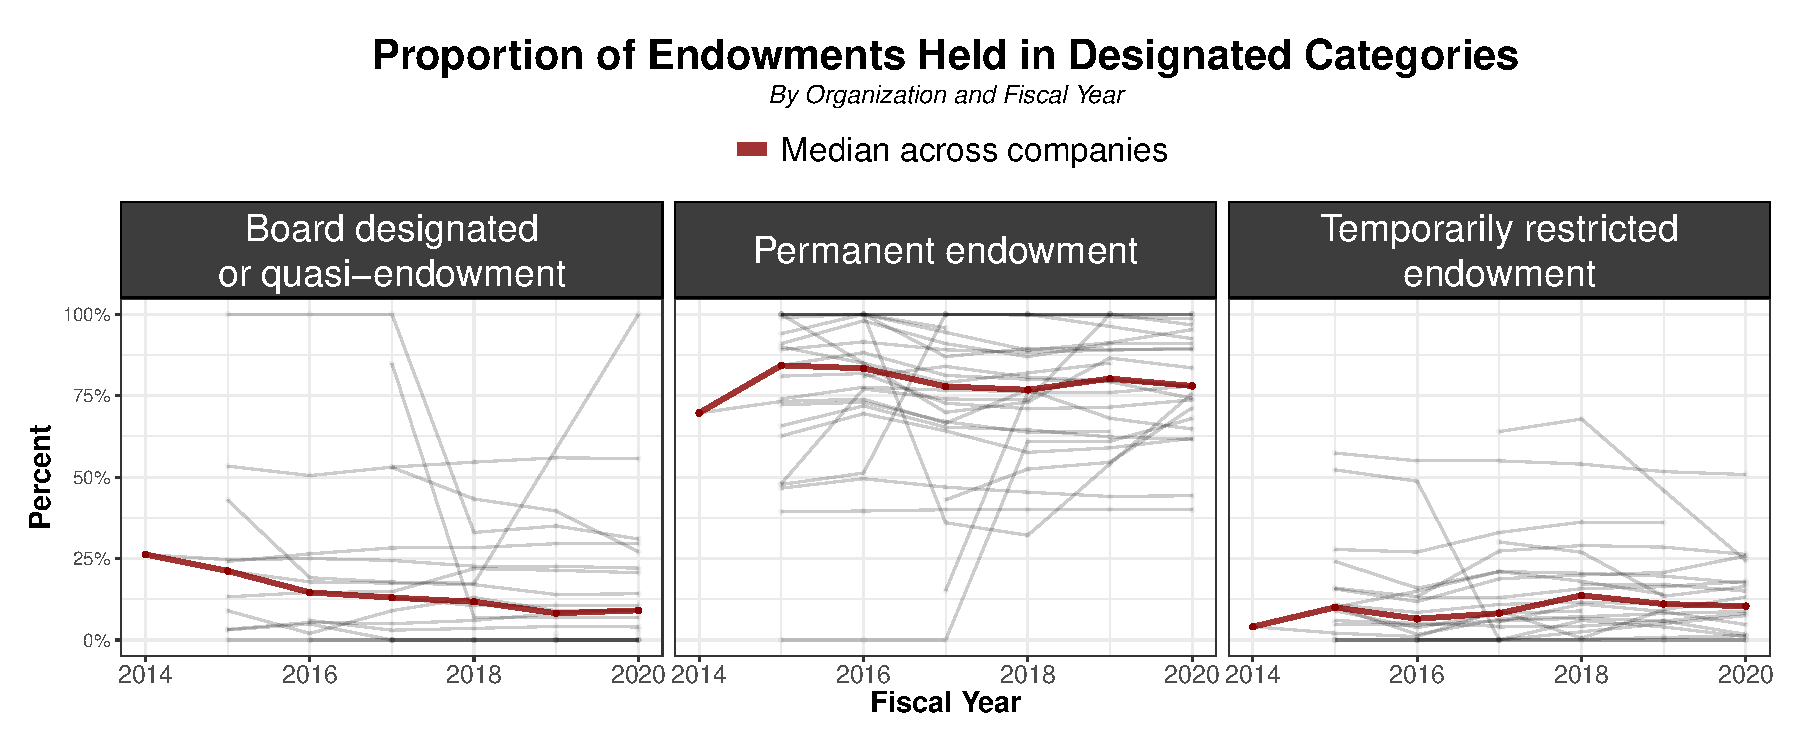
\includegraphics[width=0.9\linewidth,]{../images/proportion_endowment_categories} \caption{\label{fig:endowment-type}The percent of endowments held as a temporarily restricted endowment, permanent endowment, or board designated or quasi-endowment. The median across all companies by fiscal year is shown in red.}\label{fig:proportion-endowment-categories}
\end{figure}

However, there are several notable exceptions to the general trend of
consistency across years. Defining variability as the maximum standard
deviation of the proportions for each category, the most variable 5
companies were Fort Wayne Ballet, San Francisco Ballet, Nashville
Ballet, Atlanta Ballet, and the Washington Ballet (Figure
\ref{fig:prop-most-variable}).

\begin{itemize}
\item For Fort Wayne Ballet, most of the endowment funds (86\%) were board designated/quasi-endowment in 2017, but this dropped to a mere 7\% in 2018. The percentage of the endowment funds in the permanent endowment category increased accordingly. 
\item 100\% of San Francisco Ballet’s endowment was in the board designated/quasi-endowment category up until 2018, when the percentage in  board designated/quasi-endowment  dropped to 33\% and most (61\%) was a permanent endowment.
\item  The trends in Nashville Ballet’s endowment went the opposite direction, with a large increase in the percentage in the  board designated/quasi-endowment  category (17\% to 74\%) and decrease in the percentage in the permanent category.
\item For Atlanta Ballet, there is a dramatic shift in 2017 where the percentage held as temporarily restricted goes from 0\% to 64\%.
\item The Washington Ballet had a high proportion of its endowment in the temporarily restricted category (52\%) but by 2017 all their endowment funds were in the permanent endowment category. 
\end{itemize}

\begin{figure}[H]
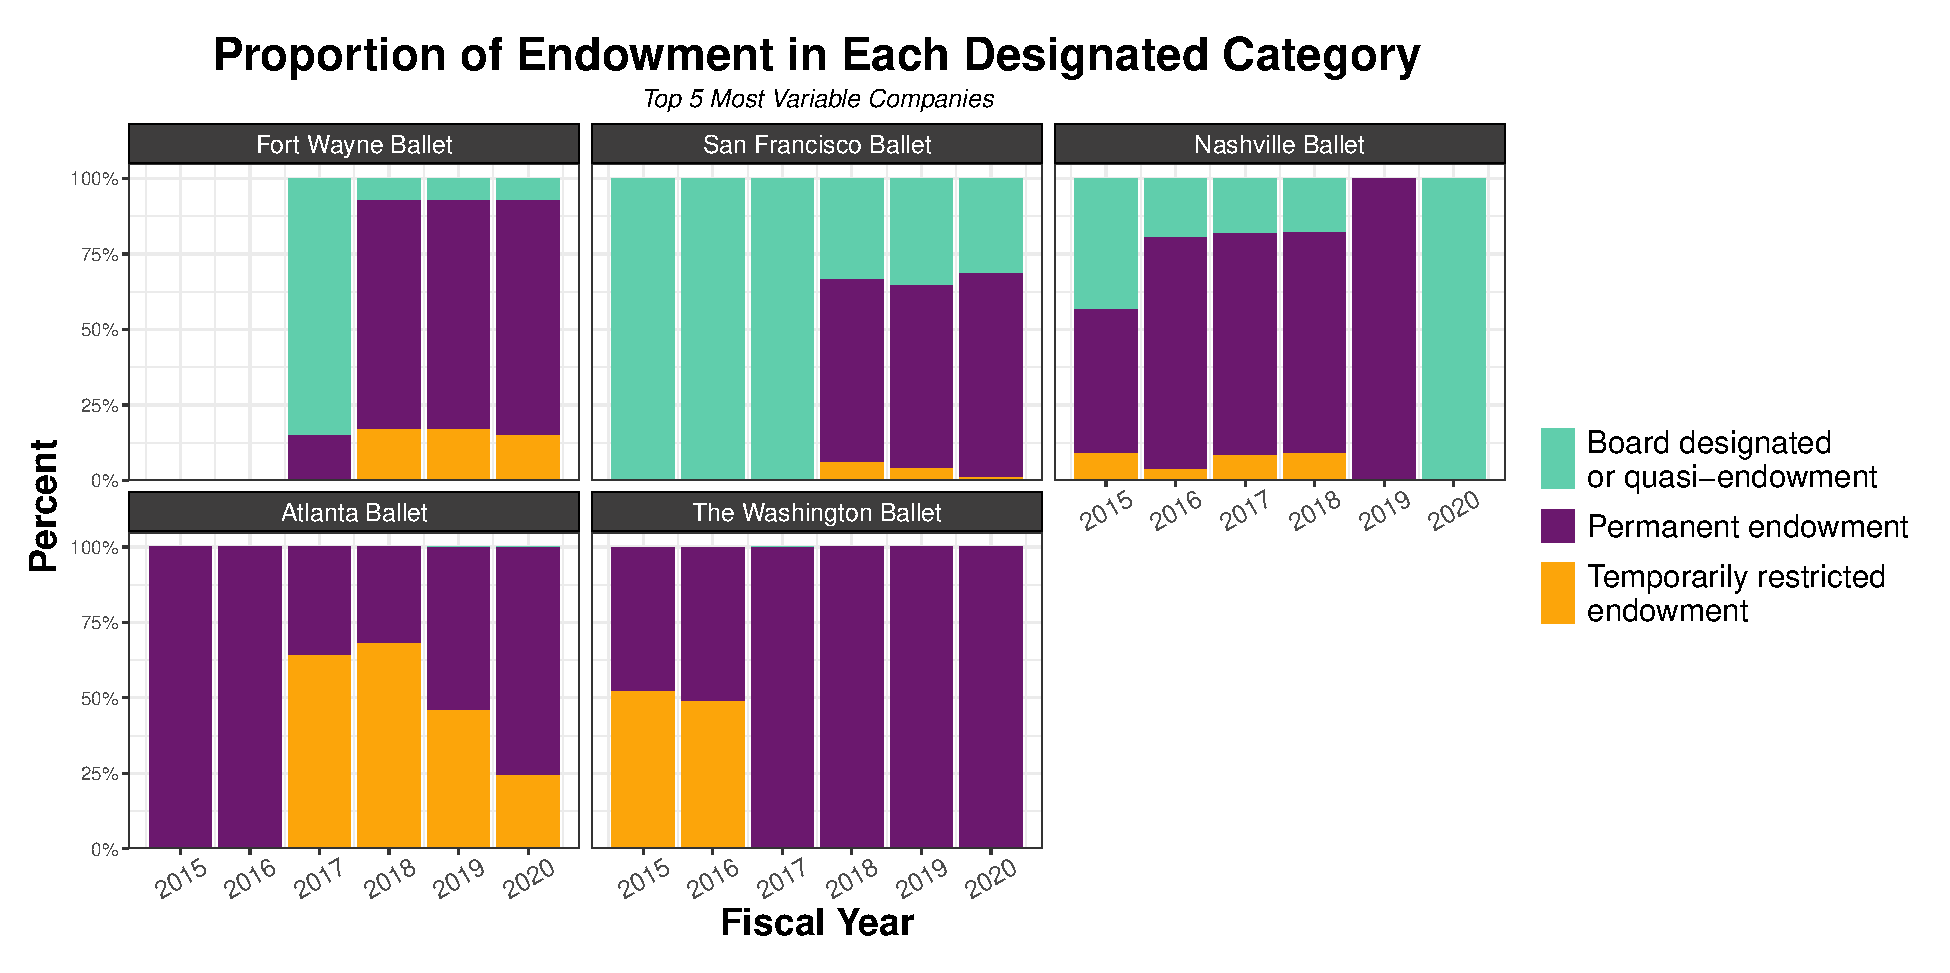
\includegraphics[width=0.9\linewidth,]{../images/prop_endowment_type_most_variable} \caption{\label{fig:prop-most-variable} Proportions of endowments in each designated category over time for the 5 companies with the most variability. The most variable companies is defined by considering the maximum standard deviation in the proportion in any one category.}\label{fig:proportion-endowment-categories-most-variable}
\end{figure}

\hypertarget{which-companies-have-endowments}{%
\subsubsection{Which Companies Have
Endowments?}\label{which-companies-have-endowments}}

One of the most fundamental questions about endowments is how many
companies report them, and how the number of companies reporting
endowments varies over time. To report endowments, nonprofits fill out
Schedule D in Form 990. Out of the 169 dance companies investigated, 47
reported endowments at least once in Schedule D (Table
\ref{table:filled-scheduled}).

\begin{table}[!h]

\caption{\label{tab:unnamed-chunk-2}\label{table:filled-scheduled}Number of Companies that Reported an Endowment}
\centering
\begin{tabular}[t]{>{\raggedright\arraybackslash}p{10em}>{\raggedleft\arraybackslash}p{10em}>{\raggedleft\arraybackslash}p{10em}}
\toprule
 & Reported an Endowment & Did Not Report an Endowment\\
\midrule
\addlinespace[0.5em]
\multicolumn{3}{l}{\textbf{By Year}}\\
\hline
\hspace{1em}2014 & 1 & 6\\
\hspace{1em}2015 & 35 & 70\\
\hspace{1em}2016 & 37 & 79\\
\hspace{1em}2017 & 42 & 83\\
\hspace{1em}2018 & 40 & 96\\
\hspace{1em}2019 & 40 & 106\\
\hspace{1em}2020 & 40 & 83\\
\hspace{1em}2021 & 6 & 21\\
\addlinespace[0.5em]
\multicolumn{3}{l}{\textbf{\makecell[l]{Reported an Endowment\\at Least Once}}}\\
\hline
\hspace{1em} & 47 & 122\\
\bottomrule
\end{tabular}
\end{table}

\hypertarget{consistency-of-endowment-reporting}{%
\subsubsection{Consistency of Endowment
Reporting}\label{consistency-of-endowment-reporting}}

In investigating the frequency of reporting endowments, it is apparent
that most companies who report an endowment continue to consistently do
so across their 990 filings (Figure \ref{fig:gap-plot}). Some, however,
including Oregon Ballet Theater and Ballet Des Moines, begin reporting
an endowment well after their first filed 990. Other companies such as
The Charleston Ballet, Colorado Ballet, and American Repertory Ballet
stopped reporting endowments.

\begin{figure}[H]
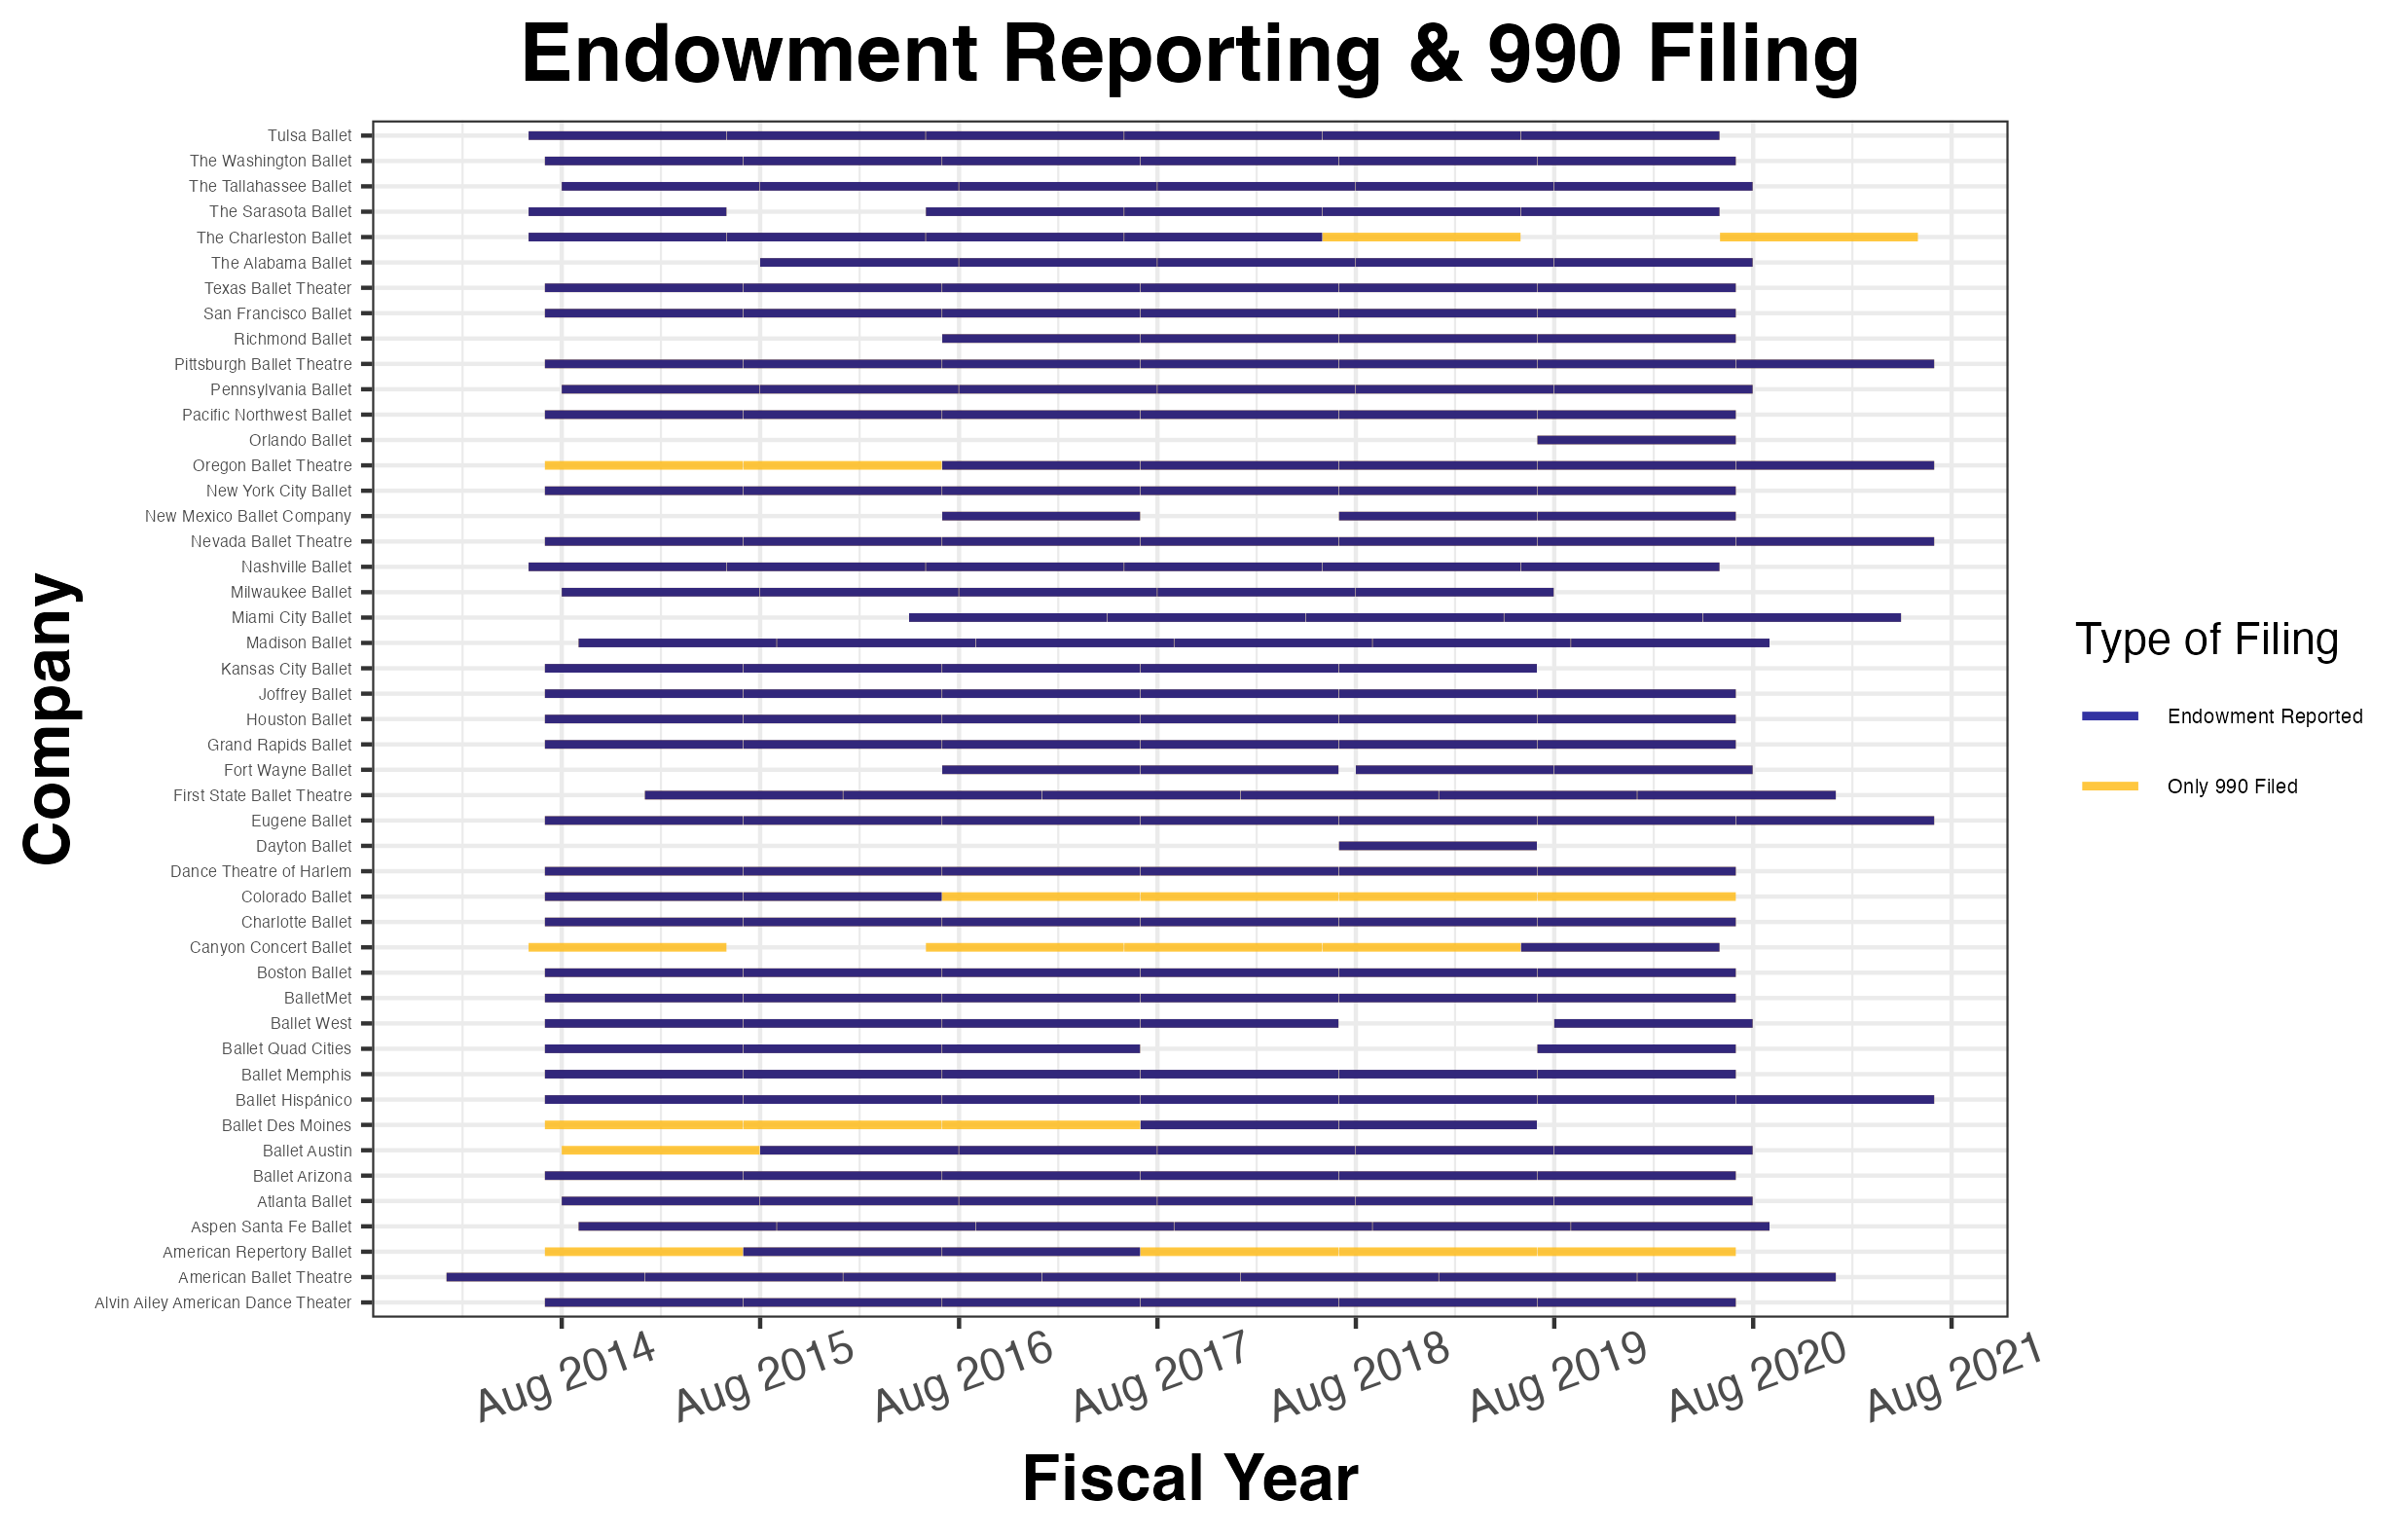
\includegraphics[width=0.9\linewidth,]{../images/gap_plot_endowment} \caption{\label{fig:gap-plot}Continuity of filings among dance companies; gaps in a companies' filings correspond to missing fiscal years.}\label{fig:unnamed-chunk-3}
\end{figure}

\hypertarget{ranking-companies-endowments}{%
\subsubsection{Ranking Companies'
Endowments}\label{ranking-companies-endowments}}

Ranking companies can be useful to see how endowments did relative to
each other rather than looking at the raw values, which are on immensely
different scales.

When viewing the rankings of the beginning of year balance of companies'
endowments, it is immediately apparent that the top 7 companies, New
York City Ballet, San Francisco Ballet, Houston Ballet, Alvin Ailey
American Dance Theater, American Ballet Theatre, Pacific Northwest
Ballet, and Boston Ballet, see no changes in ranking from 2013 to 2020
(Figure \ref{fig:rank-endowments}).

Below the top 7, there are more shifts in the rankings across time, with
some companies changing dramatically in ranking. This includes:

\begin{itemize}
\item A dramatic decrease in Aspen Santa Fe Ballet’s ranking from 2018 through 2020, due to the company’s decisions noted  \hyperref[sec:asfb]{previously}.
\item A marked increase in: 
\subitem - Joffrey Ballet’s ranking
\subitem - Orlando Ballet’s ranking
\subitem - Fort Wayne Ballet’s ranking
\subitem - Ballet Arizona’s ranking
\item A decrease in Atlanta Ballet’s ranking from 2013 to 2015 that then recovered.
\end{itemize}

\begin{figure}[H]
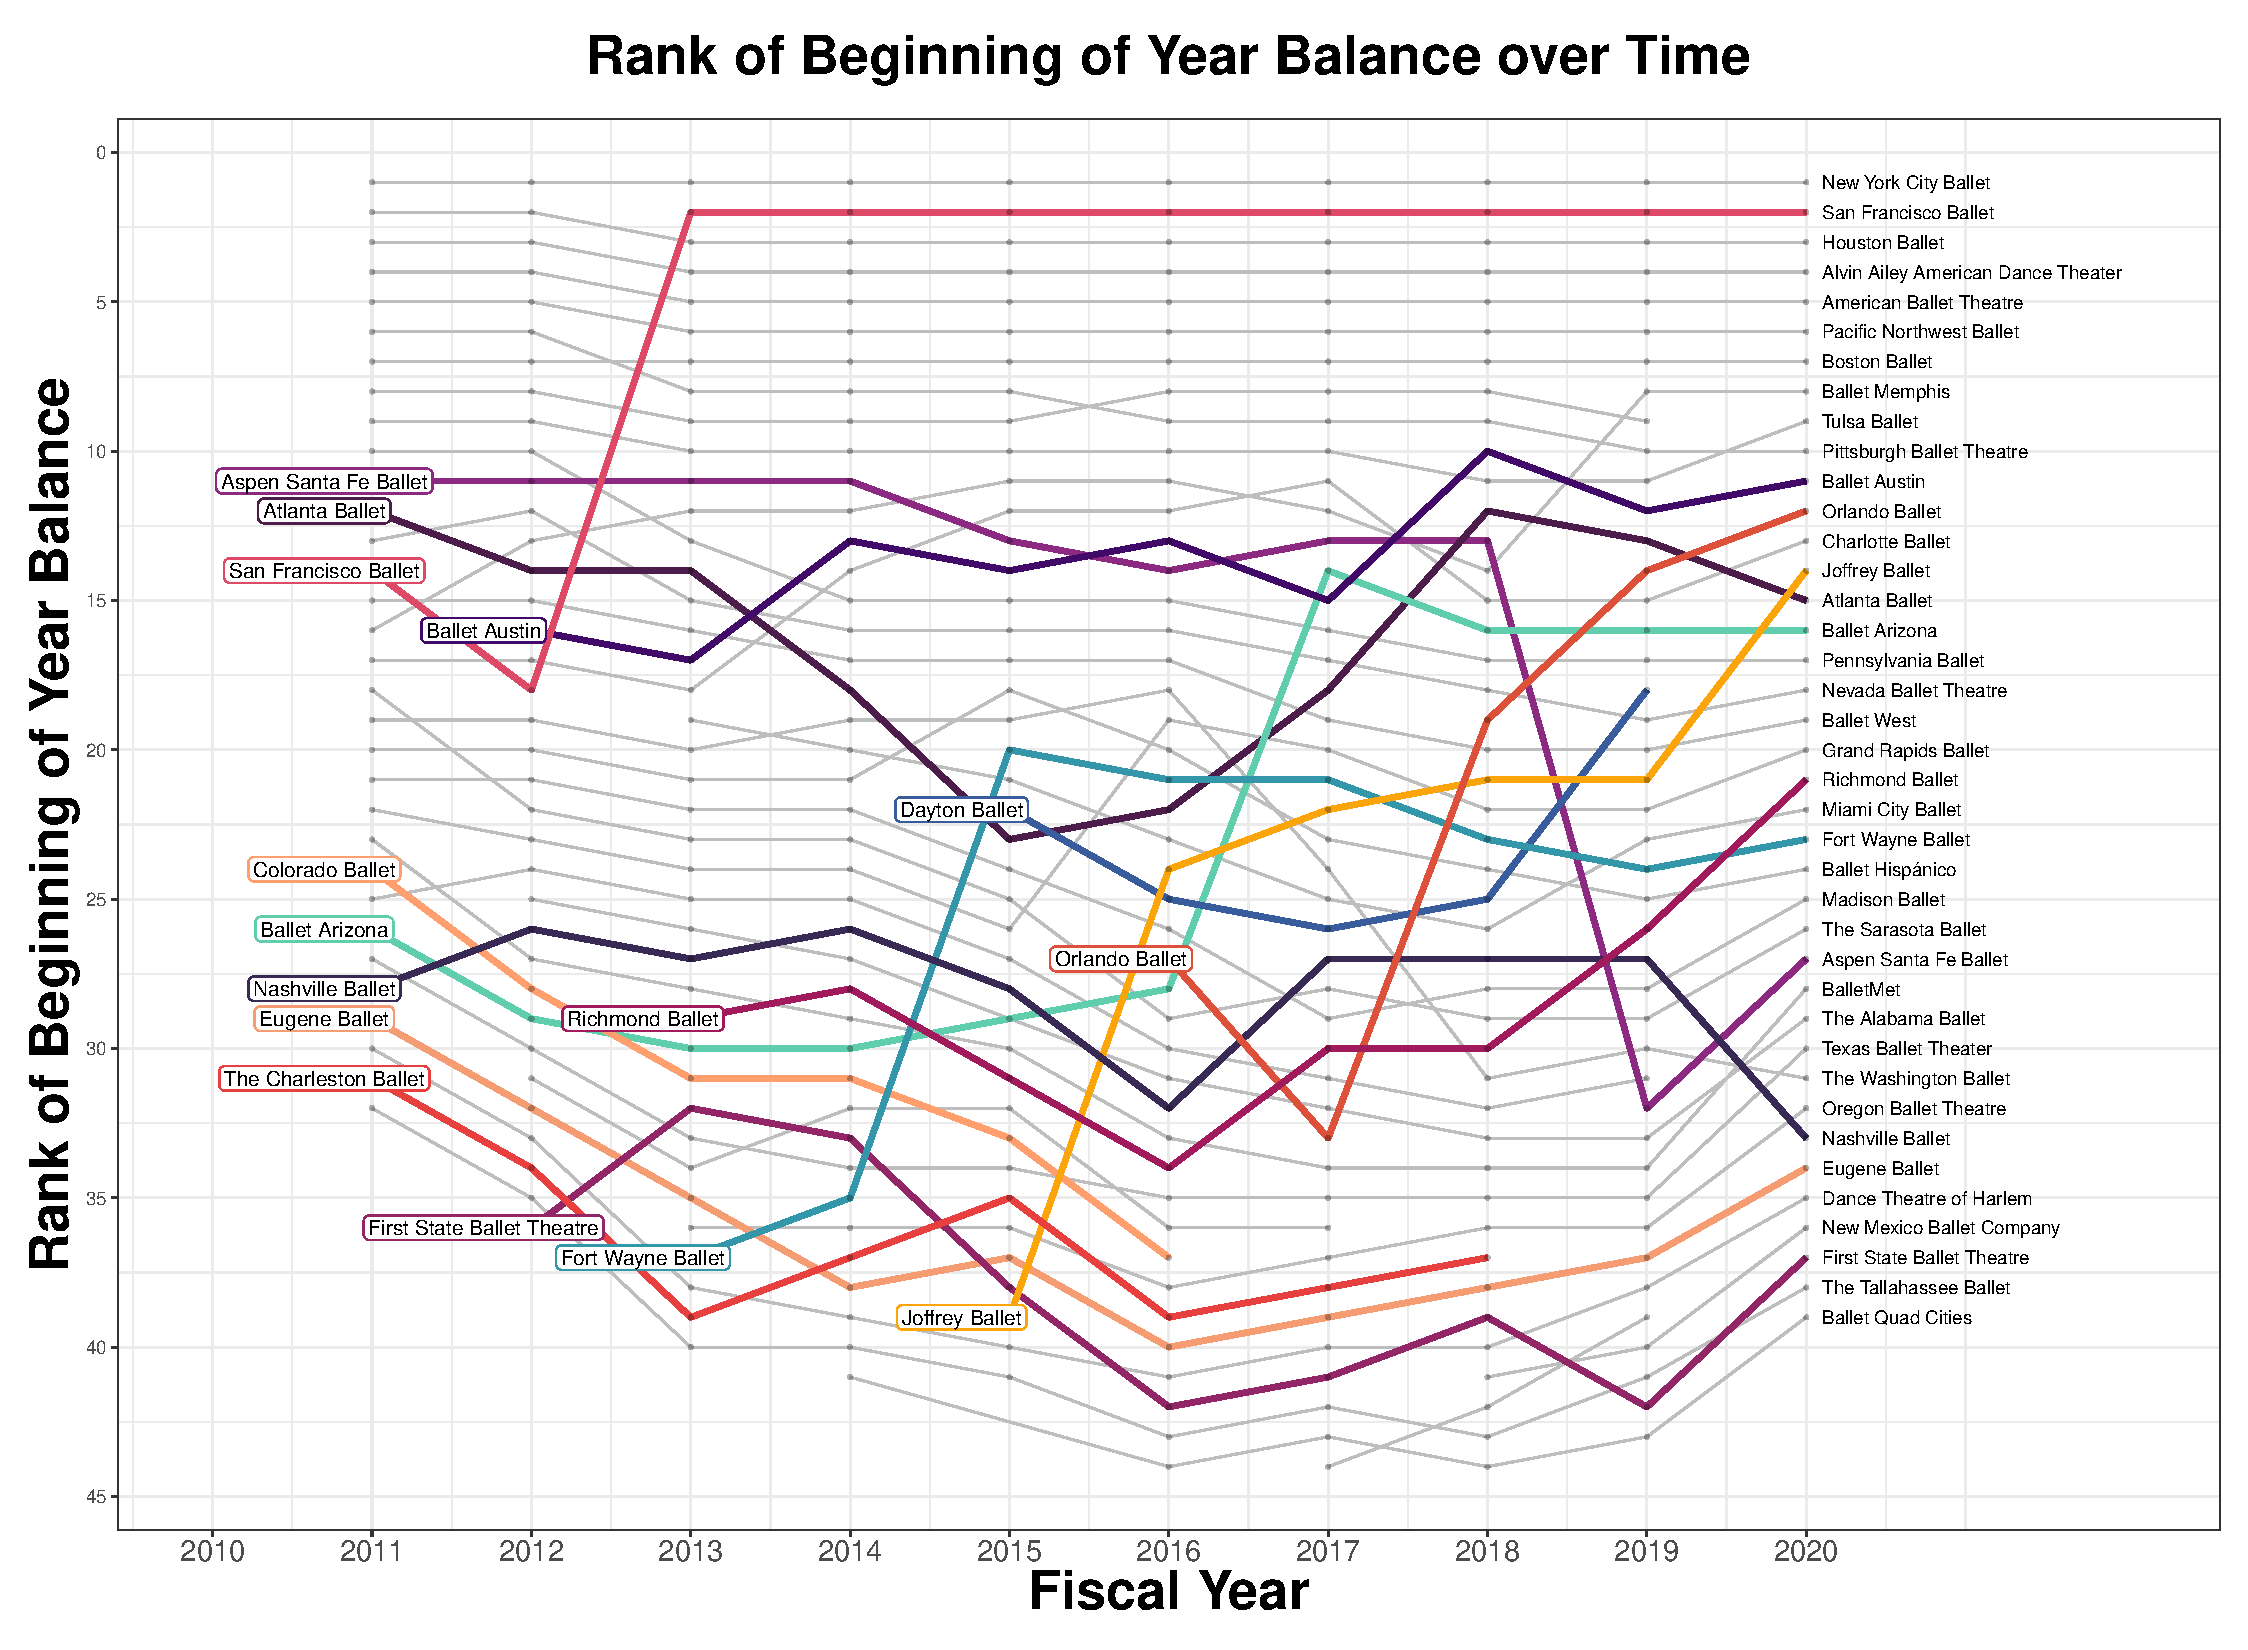
\includegraphics[width=0.9\linewidth,]{../images/rank_of_beginning_year_balance} \caption{\label{fig:rank-endowments}Rank of the endowment beginning of year balance over time. The 15 companies with the most variability in ranking, defined as the mean difference in rankings between fiscal years, are shown in color. Names of all companies are on the right.}\label{fig:rank-og-beginning-year-balance}
\end{figure}

The relationship between contributions and endowments warrants
exploration since both of these sources of funds can enhance a company's
financial well-being.

When the lines for each company from Figure \ref{fig:rank-endowments}
are colored by how these companies ranked in contributions (Figure
\ref{fig:rank-endowments-color-contribution}), a couple of trends are
clear. For one, companies that are ranked high in endowments tend to
rank high in contributions; for example, New York City Ballet is
top-ranked in both endowments and contributions. Similarly, companies
ranking low in endowments tend to rank low in contributions.

Notably, several of the companies that experienced notable changes in
their rankings also were ranked high in contributions, in particular,
Orlando Ballet and Joffrey Ballet.

High contributions, in these cases, may have contributed to Orlando
Ballet's and Joffrey Ballet's enormous growth in their endowments across
time, which may enhance their financial stability in years to come.

Understanding how contributions relate to changes in endowment balances
is important in understanding how these contributions impact companies
long-term.

\begin{figure}[H]
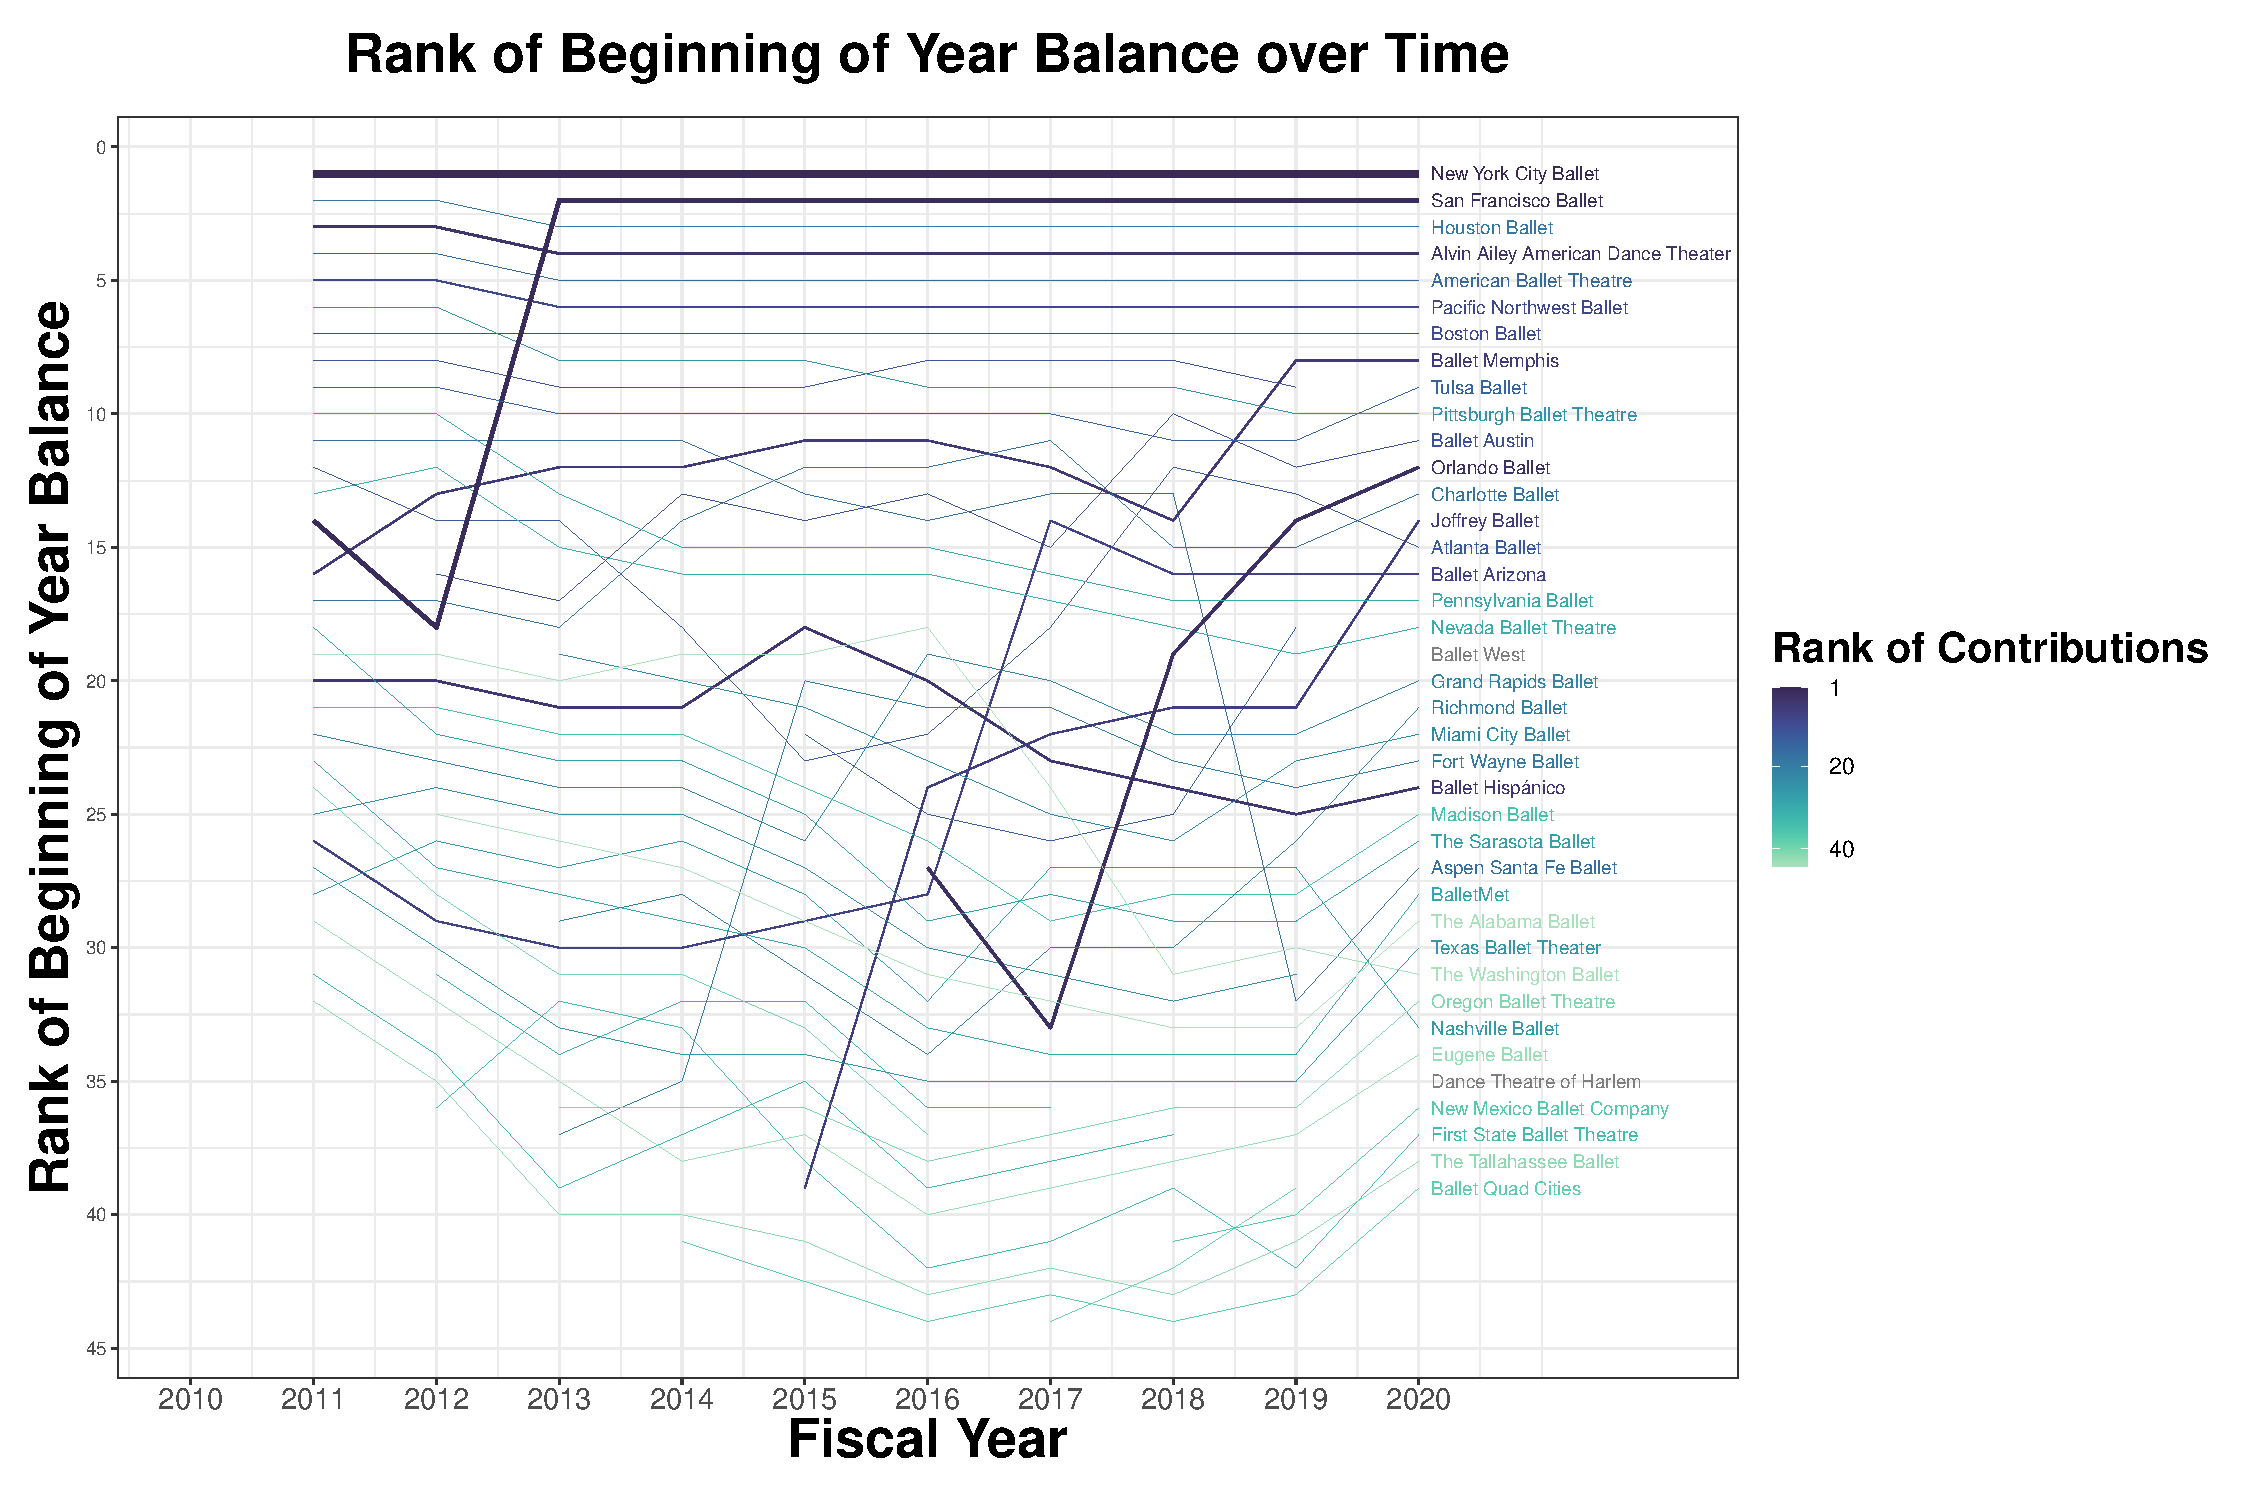
\includegraphics[width=0.9\linewidth,]{../images/rank-endowments-color-contribution} \caption{\label{fig:rank-endowments-color-contribution}Rank of the endowment beginning of year balance over time, where the color indicates the ranking of the mean contributions received over all years on file for the company.}\label{fig:unnamed-chunk-4}
\end{figure}

Looking more closely at the relationship between contribution rankings
and beginning-of-year balance rankings, in Figure \ref{fig:balancecont},
there is a strong relationship between how a company ranks with regard
to their contributions relative to the other companies and how a company
ranks in the endowment beginning of year balance. That is, when
companies are ranked high at the beginning of the year balance, they
tend to rank high in contributions as well. As expected, this trend
holds across the full set of fiscal years considered.

However, the rankings are often not identical. If they were, all points
would fall on the red line, which represents an exact correspondence
between rankings. In some cases, a company consistently ranks higher in
contributions relative to the beginning-of-year balance. Whether the
contributions or beginning-of-year balance tends to rank higher for a
given company is summarized in Figure \ref{fig:balancecontbar}. For
example, Ballet West ranked higher in the endowment beginning-of-year
balance for each year available (2016 - 2020), while Nashville Ballet
ranked higher in contributions than the beginning-of-year balance for
every year on file (2011 - 2022).

\begin{figure}[H]
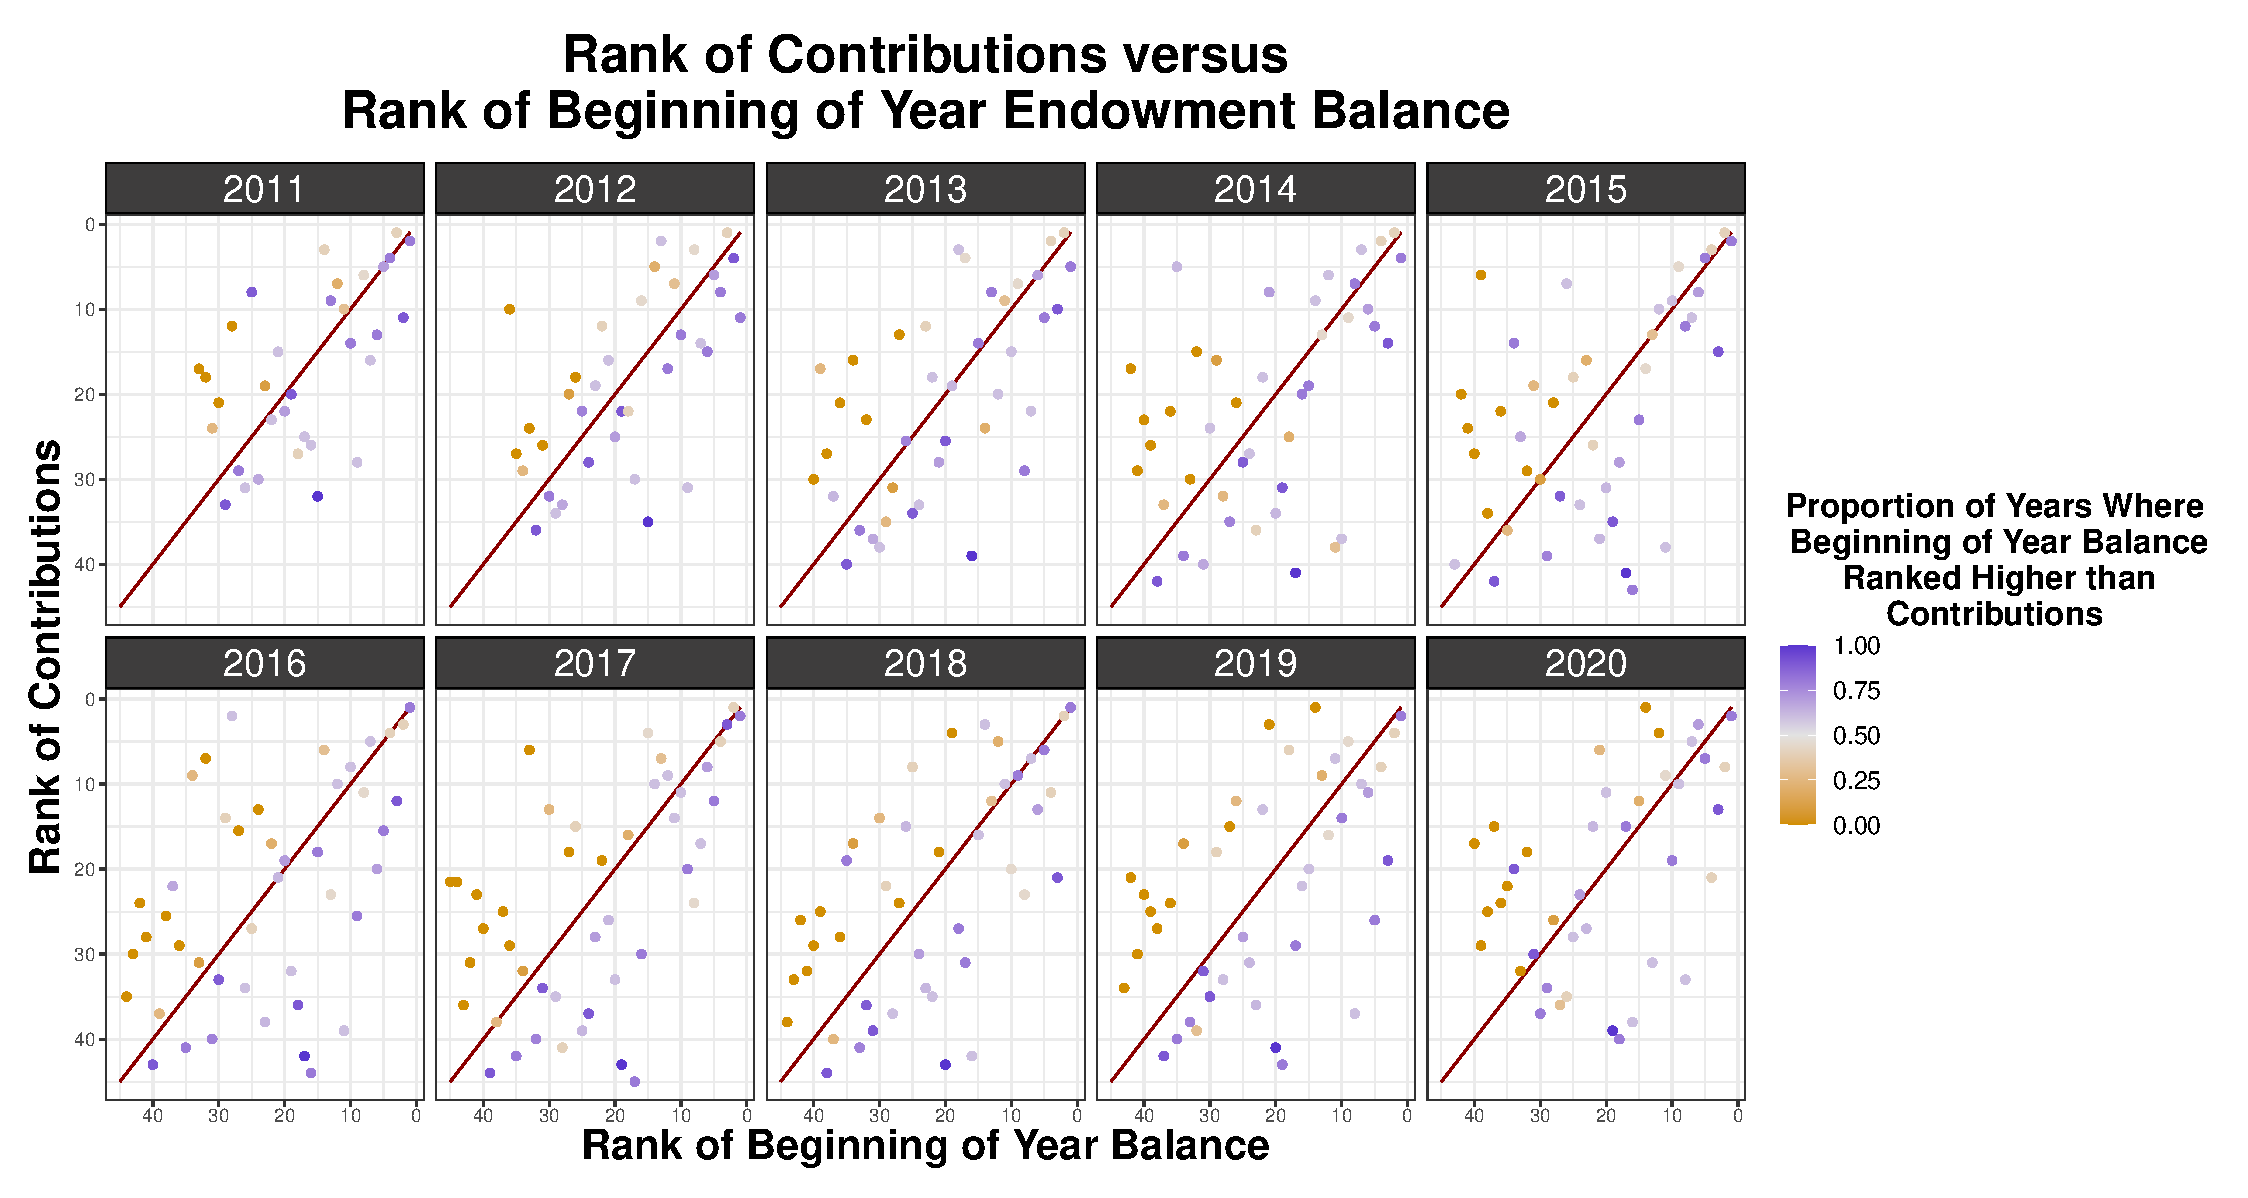
\includegraphics[width=0.75\linewidth,]{../images/compare-rankings-balance-contributions} \caption{\label{fig:balancecont} Comparing the rankings of beginning of year balance of the endowment to the ranking of contributions recieved.}\label{fig:compare-rankings-balance-contributions}
\end{figure}

\begin{figure}[H]
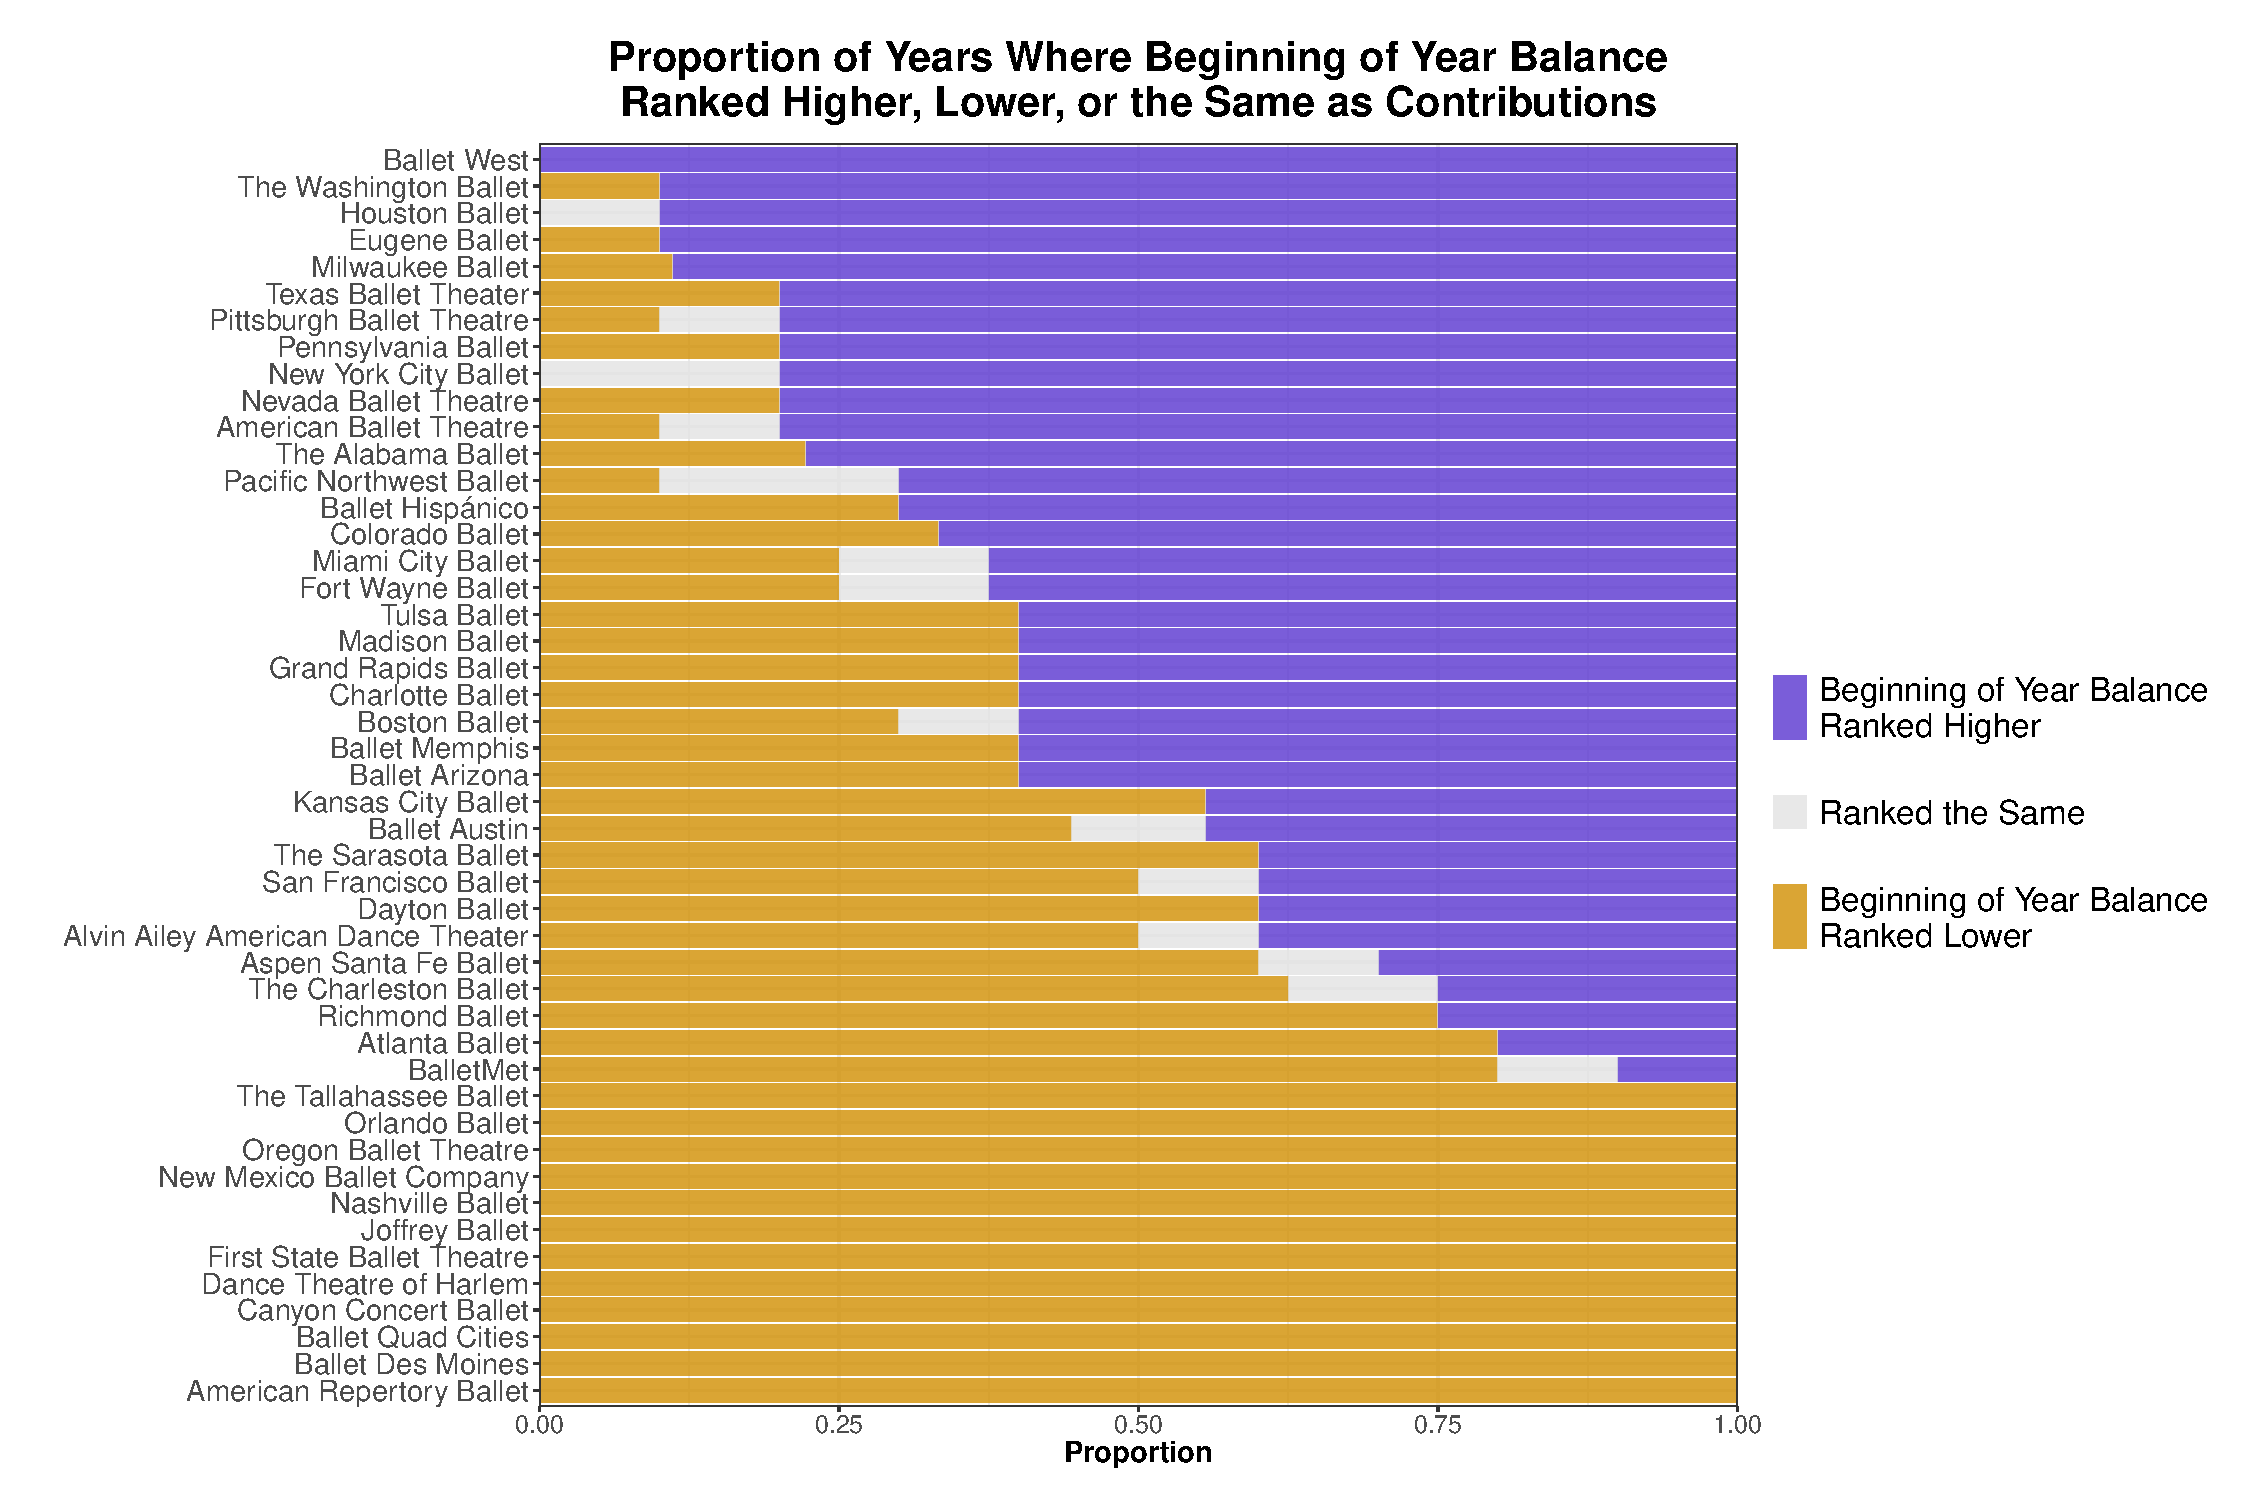
\includegraphics[width=0.75\linewidth,]{../images/compare-rankings-balance-contributions-barplot} \caption{\label{fig:balancecontbar} Comparing the proportion of years where a company ranked higher, lower, or the same in beginning of year balance compared to contributions received. A higher rank means a rank closer to 1, where 1 is the top possible rank.}\label{fig:compare-rankings-balance-contributions-barplot}
\end{figure}

In contrast to the observations in the rankings of the beginning of year
balance (Figures \ref{fig:rank-endowments-color-contribution} and
\ref{fig:rank-endowments}), Figure \ref{fig:rankings-contributions}
demonstrates that the rankings of contributions are much less
consistent. It is clear that contributions are a less stable source of
funding for these companies, and the amount companies receive year to
year varies considerably.

\begin{figure}[H]
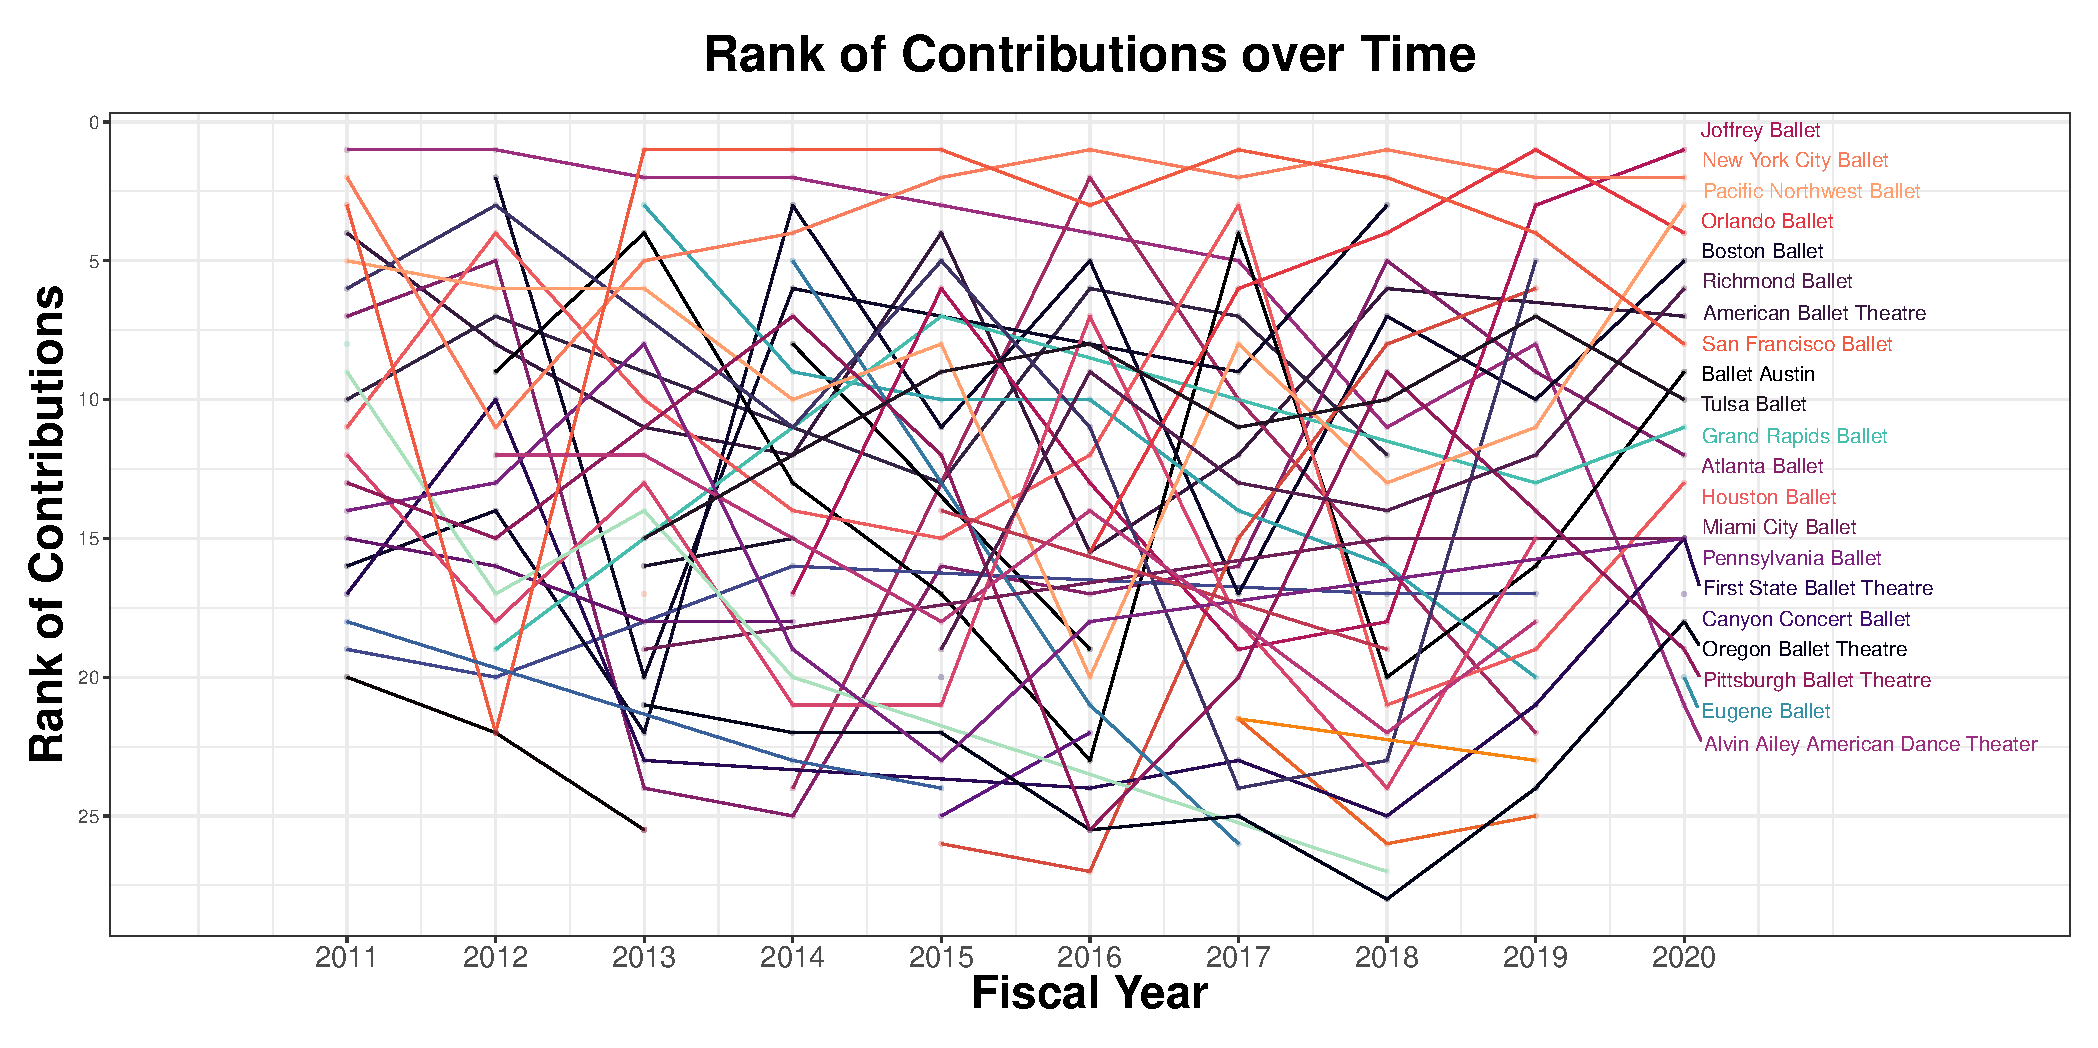
\includegraphics[width=0.9\linewidth,]{../images/ranking-contributions} \caption{\label{fig:rankings-contributions}The rankings of contributions over time, by organization.}\label{fig:ranking-contributions}
\end{figure}

\hypertarget{not-to-be-published-reported-endowment-balances-over-time---is-the-math-right}{%
\subsubsection{NOT TO BE PUBLISHED: Reported Endowment Balances over
time - Is the Math
right?}\label{not-to-be-published-reported-endowment-balances-over-time---is-the-math-right}}

\begin{quote}
Due to time constraints within our project, the capstone team did not
have the opportunity to reach out to any companies regarding their
miscalculations or reporting of negative expenses. The team recommends
doing this prior to this report being published.
\end{quote}

Theoretically, one can calculate an endowment's fiscal year end balance
based on all information provided in Schedule D. The end-of-year balance
was calculated (see the equation below) and then compared our calculated
balance to the reported end-of-year balance. The majority of
calculations are concordant; however, discrepancies were noted in
thirteen companies. Discrepancies range from \$-20,000 (Orlando Ballet,
2016) to \$8,301,066 (Atlanta Ballet, 2017). Due to the scaling of the
below figure, differences in reported and calculated balances below a
hundred thousand dollars are difficult to see.

\[\text{Calculated Year End Balance} = \text{Beginning Year Balance} + \text{Contributions} +\]
\[ \text{Investment Earnings or Losses} - |\text{Administrative Expenditures}| -\]
\[|\text{Other Expenditures}| - | \text{Grants or Scholarships}| \tag{1}\]

For values related to expenses (administrative expenditures, other
expenditures, grants, or scholarships), the absolute value was used to
ensure all were positive numbers. Four companies (Ballet Hispánico,
Atlanta Ballet, Miami City Ballet, and Dance Theatre of Harlem) report
their other expenditures as a negative value; thus, when calculating
end-of-year balance, subtracting a negative value would result in an
additive, not subtractive, effect.

The difference in the extent of discrepancies when the absolute value is
taken (Figure \ref{fig:miscalc} (a)), as in equation (1), versus when it
is not (Figure \ref{fig:miscalc} (b)). There are fewer discrepancies
when the absolute value is taken.

Since the difference was computed by taking
\(\text{Reported End Balance} - \text{Calculated End Balance}\),
negative values indicate the calculated end balance was larger than the
reported, and positive values indicate the reported end balance was
larger. The calculated differences are split between being negative or
positive.

Atlanta Ballet has the largest discrepancy in (a); however, if the
absolute value isn't used and the negatives as is used in (b), the
values are concordant. The opposite issue occurs for Miami City Ballet,
whereby in (a) with the absolute value, they are concordant. However, in
(b) without the absolute value of expenses, they appear eight times.
Both of these situations stem from reports of negative values in an
expenses column, although they are mirrored situations. Thus, this
raises the question of how negative expenses should be dealt with.

Considering panel (a), most companies only miscalculate once; however,
there are multiple miscalculations for Fort Wayne Ballet, Atlanta
Ballet, and Ballet Arizona. Of note, some of these differences were
trivial (e.g., \$10). Eugene Ballet does not report an end-of-year
balance for 2011, yet reports a beginning balance of \$45,000, hence the
-\$45,000 difference for this year.

\begin{figure}[H]
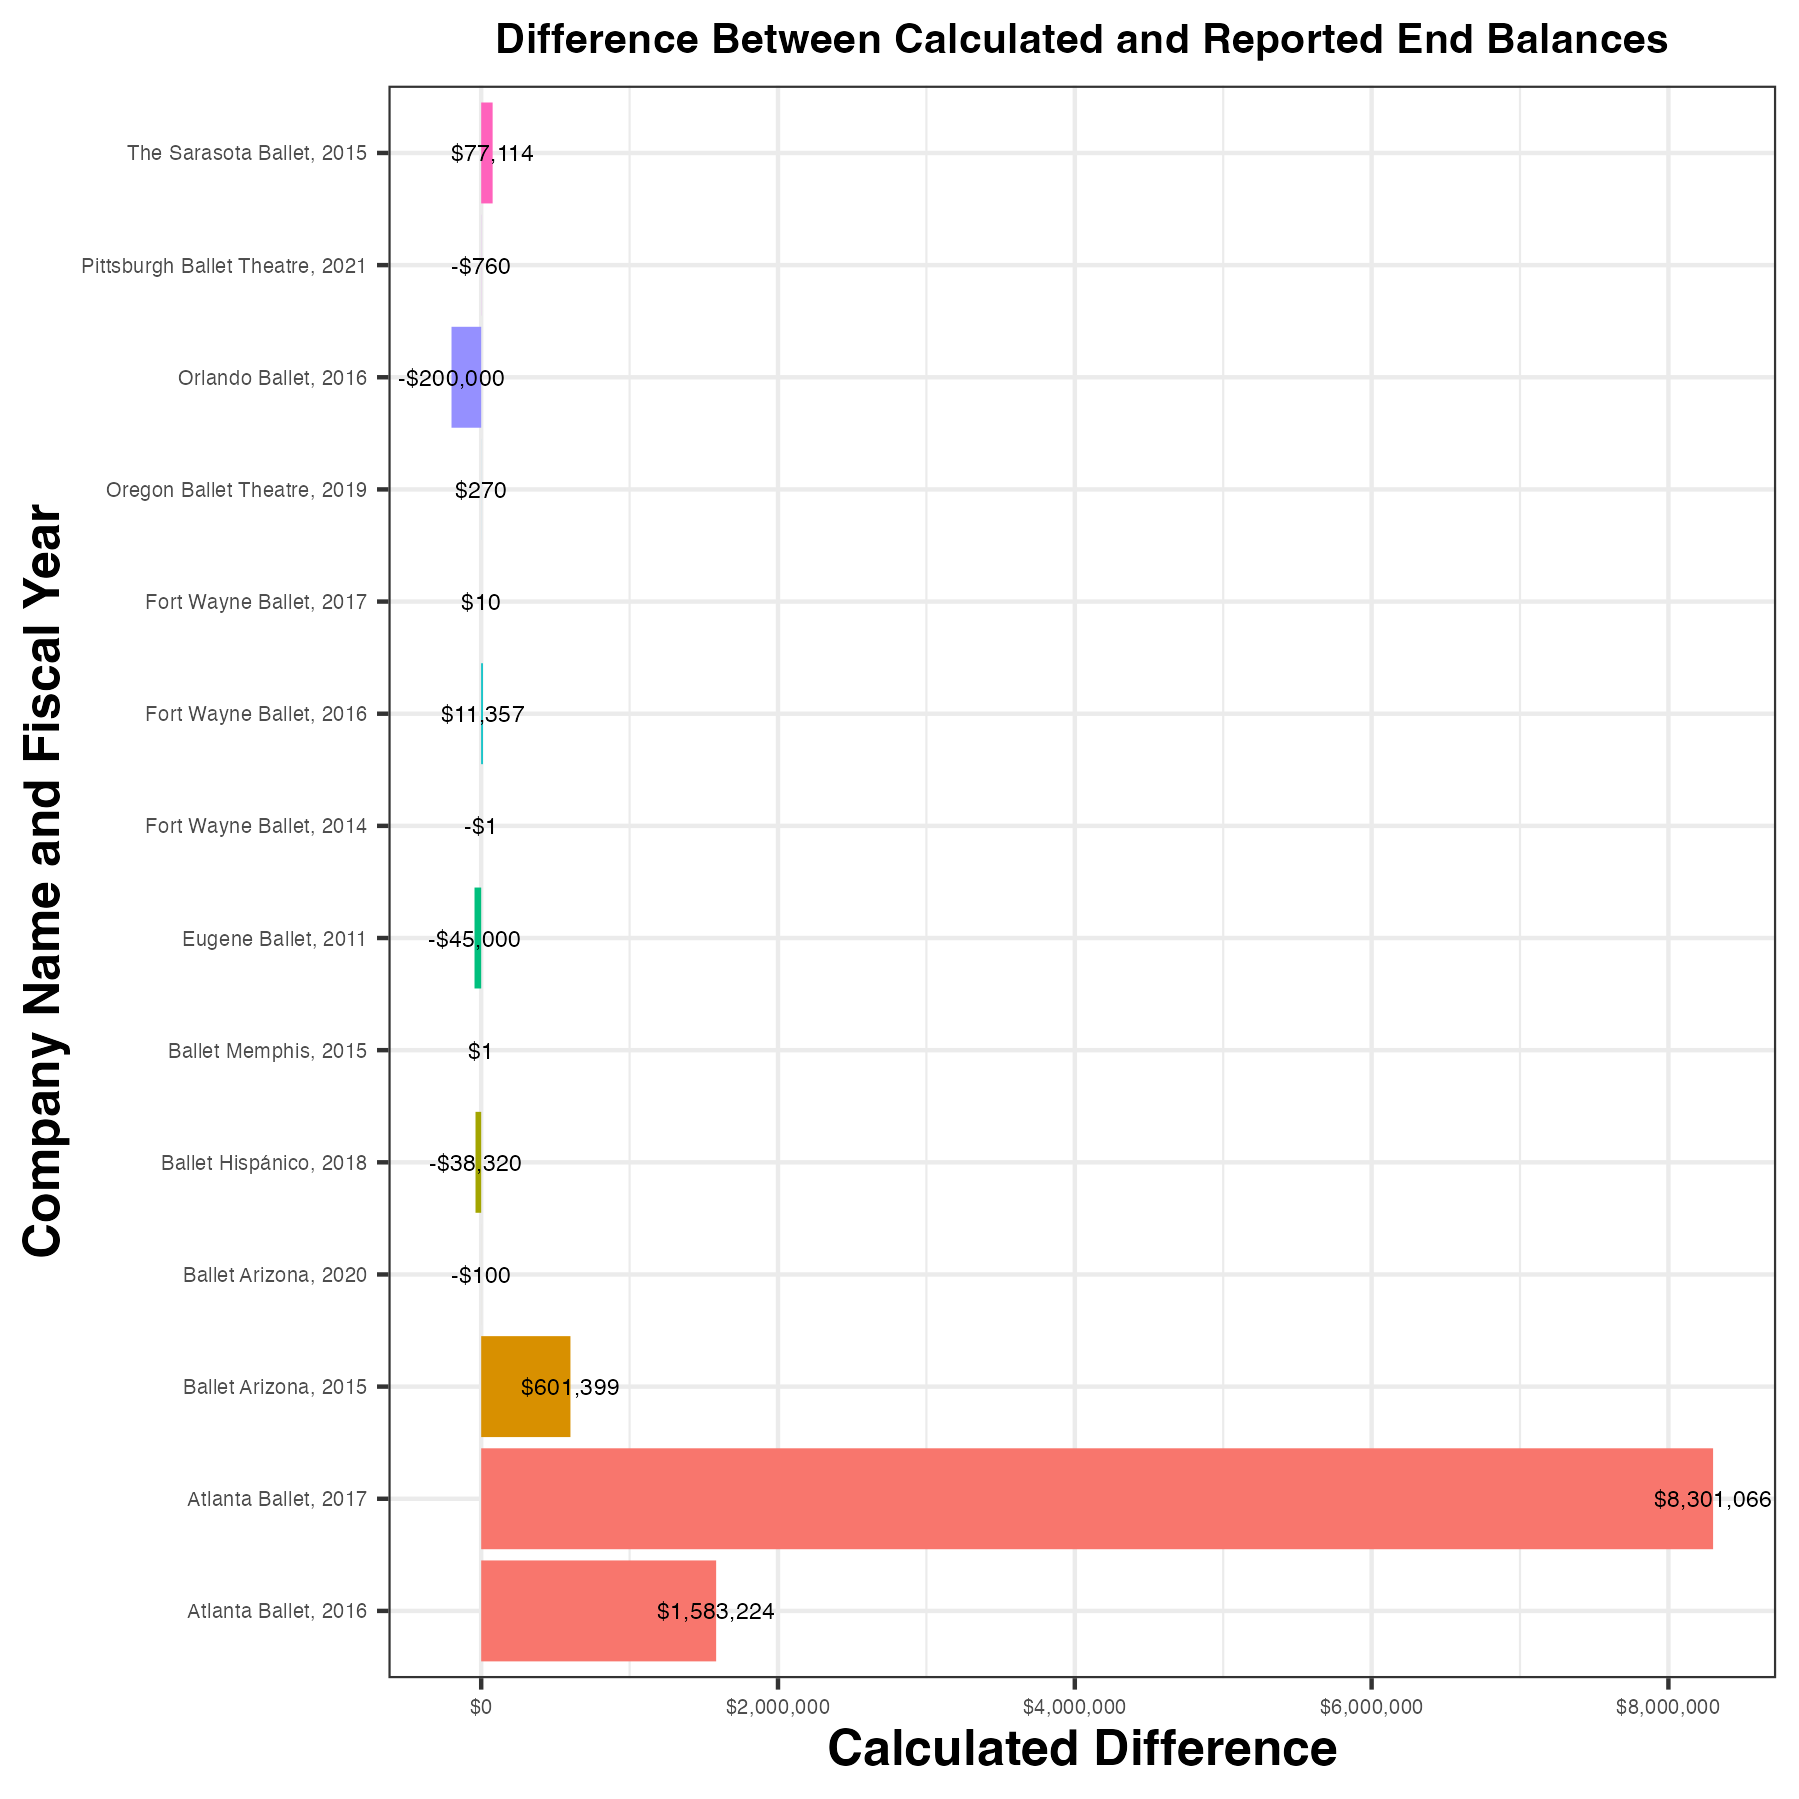
\includegraphics[width=0.5\linewidth,]{../images/diff_end_bal} 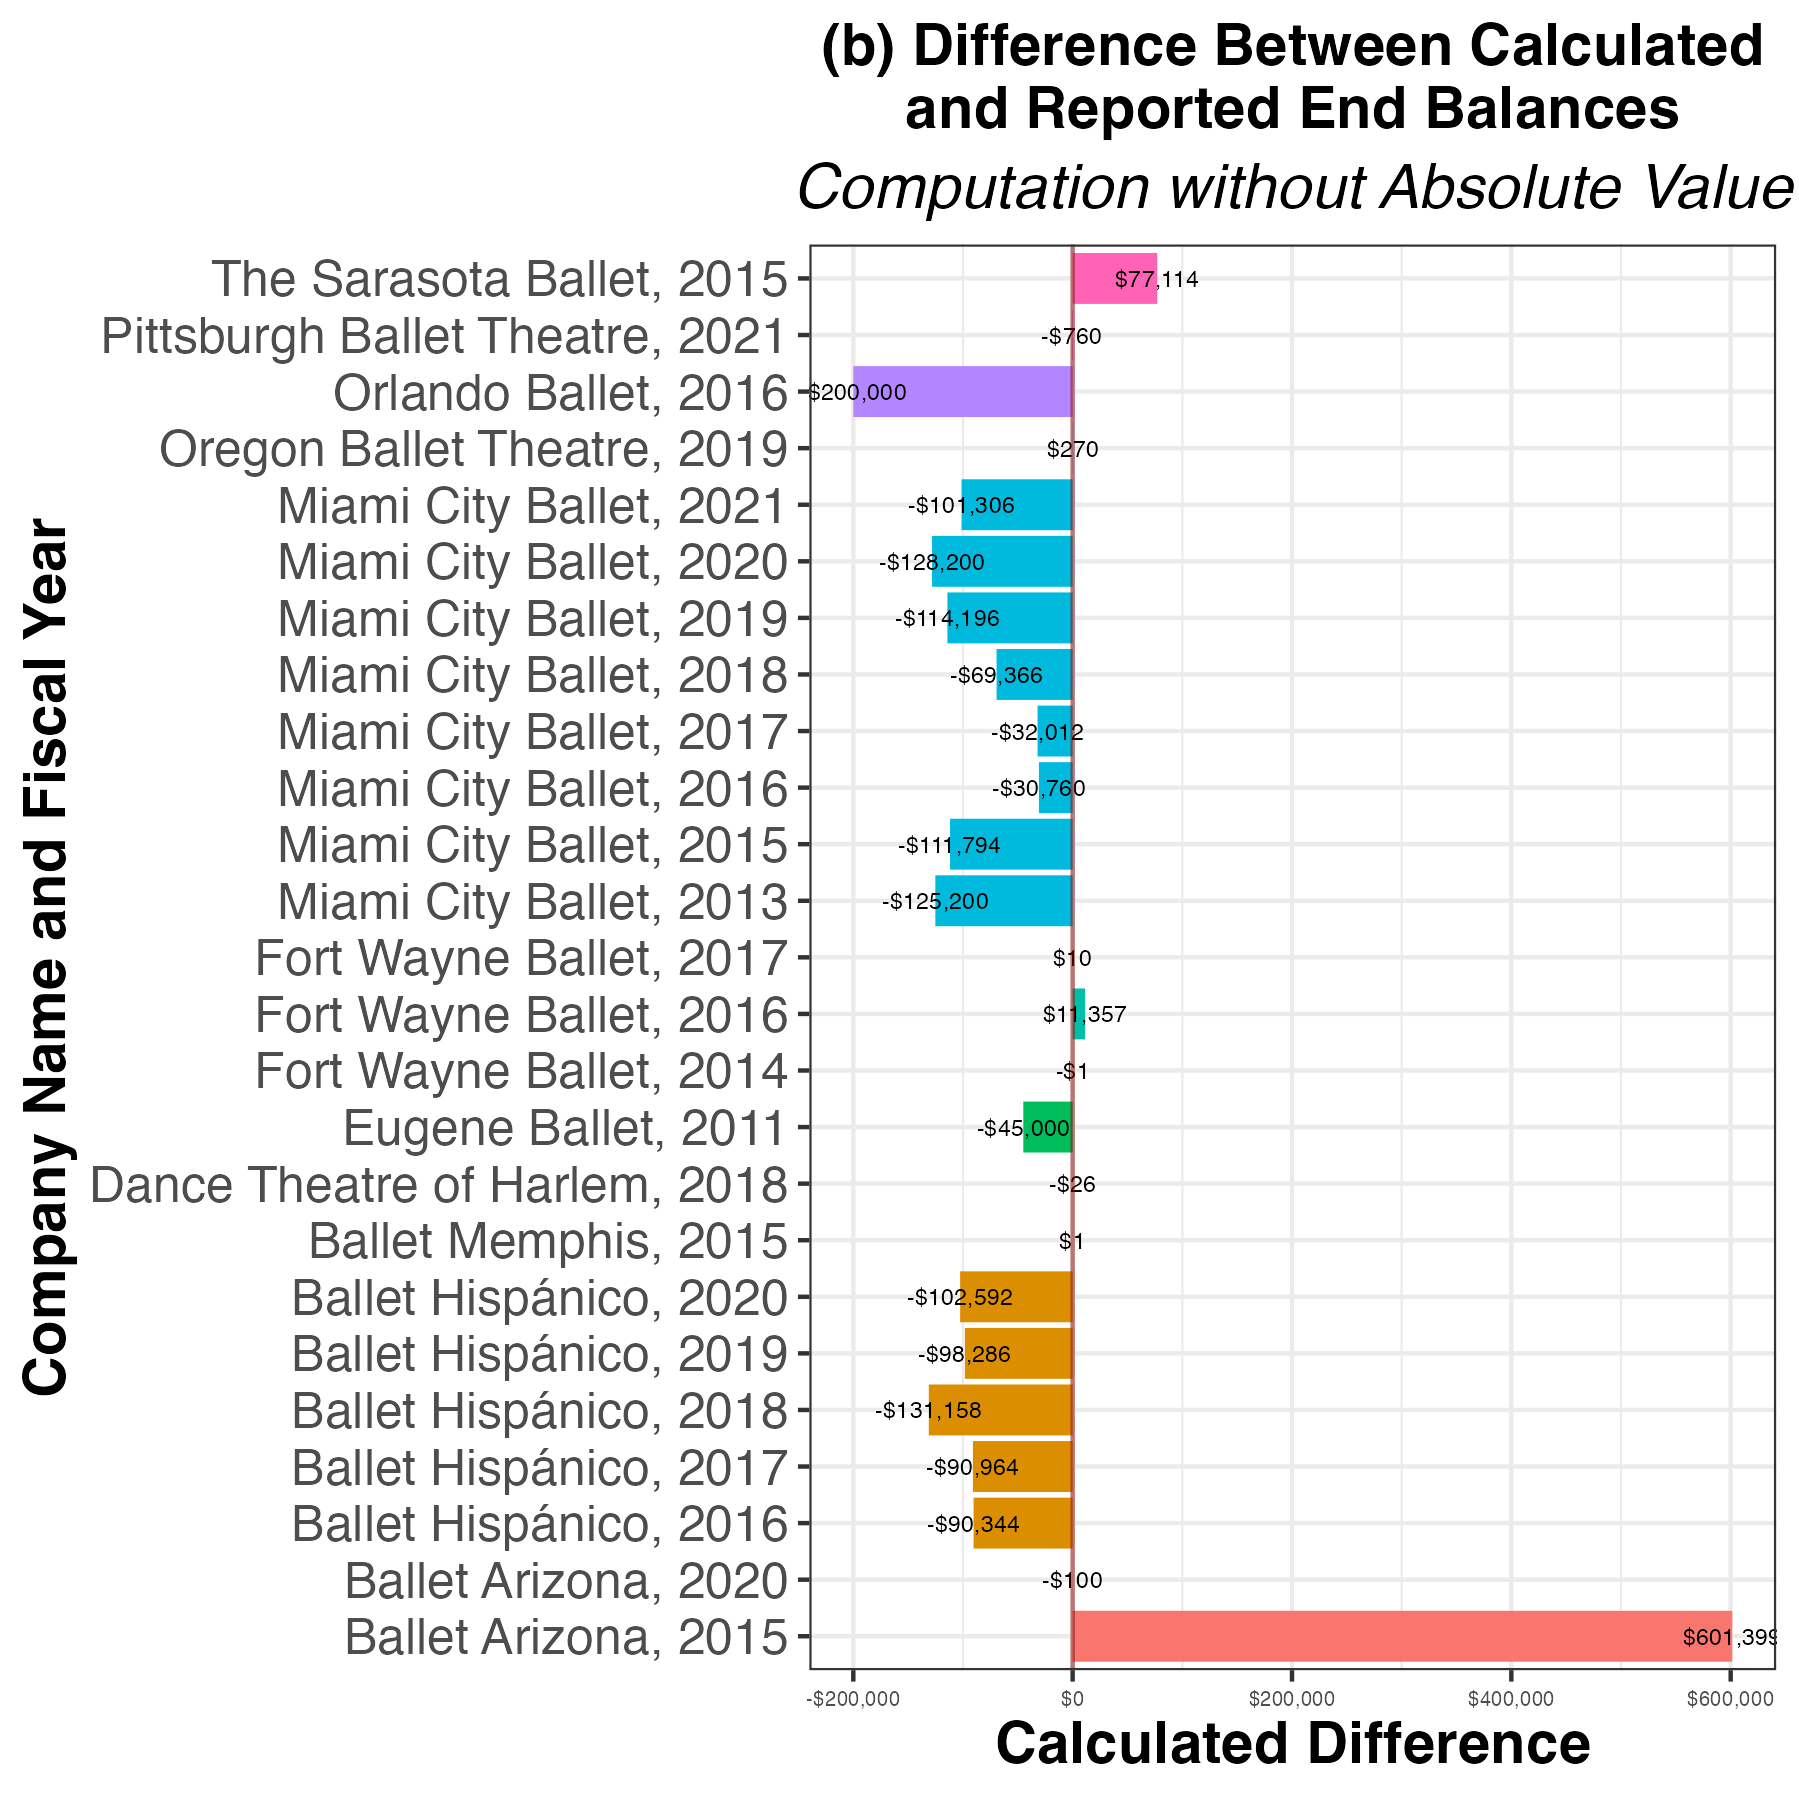
\includegraphics[width=0.5\linewidth,]{../images/diff_end_bal_no_abs} \caption{\label{fig:miscalc}Comparing the reported end of year balance to that were computed based on other reported variables. Calculation is done with the absolute value in (a) and without in (b). Each organization is in a different color.}\label{fig:unnamed-chunk-5}
\end{figure}

We summarize the discrepancies found by taking the absolute value
(e.g.~panel (a) of the above figure) in Figure
\ref{fig:miscalc-by-comp}. When taking the absolute value, the company
that misreports the most is Fort Wayne Ballet with three
miscalculations.

In future work involving end balance, the reported end-of-year balance
was utilized, as it is still uncertain how to handle negative expenses.
Thus, values that are incorrectly reported might possibly be used. End
balance is involved in calculations for two examinations in particular:
4.1.5 with Annual Percent Change and 4.1.6 Compound Growth Rate. Any
erroneous end-of-year balances will thus produce inaccurate figures.
Thus, for companies whereby an incongruence was identified (either with
or without absolute value), it is not certain whether our calculated
Compound Growth Rate or Annual Percent Change accurately reflects those
companies' endowment growth or behavior.

\begin{figure}[H]
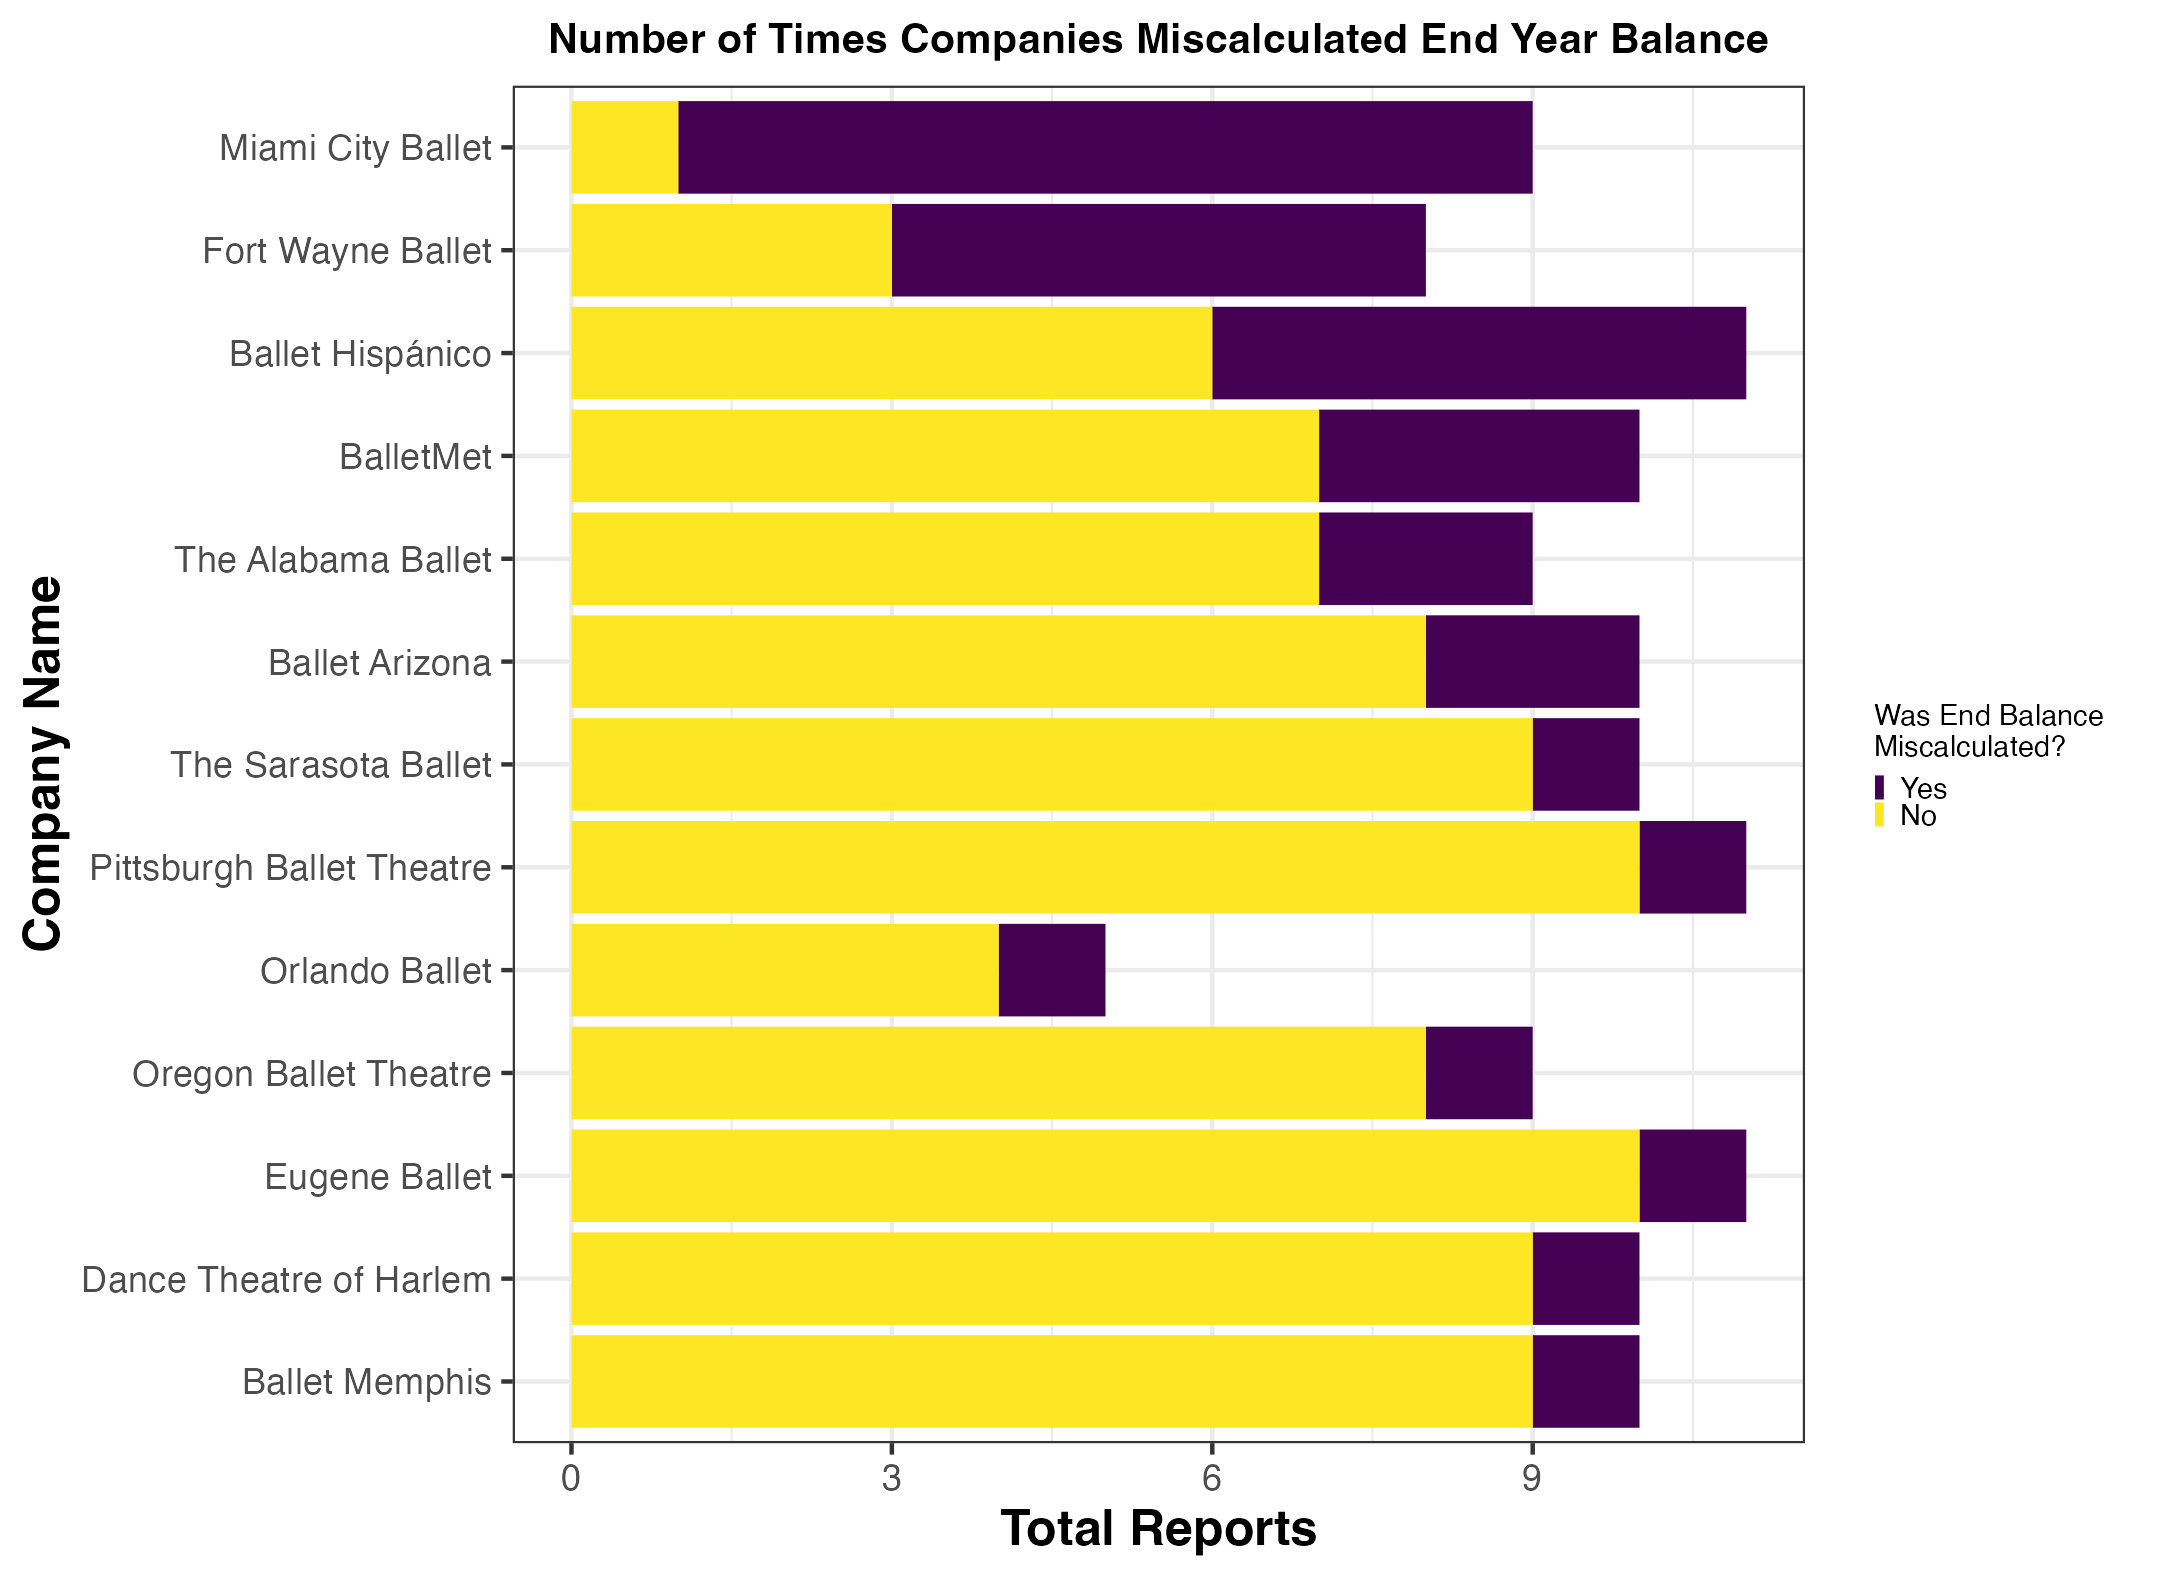
\includegraphics[width=0.5\linewidth,]{../images/miscalc_end_bal} \caption{\label{fig:miscalc-by-comp}Number of observations where there was a discrepancy between the calculated and reported end of year balance, using the absolute value equation given in equation (1).}\label{fig:miscalc-by-comp}
\end{figure}

\hypertarget{change-in-endowments-over-time}{%
\subsubsection{Change in Endowments Over
Time}\label{change-in-endowments-over-time}}

Annual percent change is the percent change from one value to the next
at the end of a year-long period. With regard to endowment balances, the
annual percent change in endowment balance is a comparison between the
endowment at the beginning of the fiscal year and the endowment at the
end of the fiscal year, which allows interpretation of the percentage by
which the endowment has grown or shrunk. Charting percent change over
time facilitates viewing endowment behavior over time; further, one can
compare percent changes between companies to get a sense of trends in
how different companies' endowments change.

With regard to the interpretation of percent change, a couple of
standard definitions are first stated.

The relative change, which represents how much a value has changed
relative to its initial value, is

\[\text{Relative change} = \dfrac{\text{End Value} - \text{Start Value}}{ \text{Start Value}}.\]

The effect of considering relative change facilitates comparison between
companies that have enormously different beginning-of-year balance
sizes. For a company with a small endowment, a difference of \$10,000
may be substantial, while the same difference would be minimal if the
company has over a million dollars in its endowment.

The percent change, which is the relative change in percentage form, is
simply \(\text{Relative Change} \times 100\).

When considering the percent change within a fiscal year, that is, from
the beginning of year balance to the end of year balance, a couple of
examples of the interpretation include\footnote{For a relative change of
  value \(R\), it can be more intuitive to interpret it by considering
  the expression \(\text{End Value} = (R+1) \times \text{Start Value}.\)
  That is, if a relative change is identified, 1 is added to it and it
  is multiplied by the starting value to acquire the end value.}:

\begin{itemize}
\tightlist
\item
  If the percent change is \(-50\%\), the endowment's value at the end
  of the fiscal year is half of what it was at the beginning.
\item
  If the percent change is \(100\%\), the endowment's value at the end
  of the fiscal year is twice what it was at the beginning.\\
\item
  If the percent change is \(-100\%\), the endowment's value dropped to
  zero throughout the fiscal year.
\end{itemize}

We calculated each company's within-year percent change of endowment
balance, as this allows for comparison of the performance of different
companies' endowments over time. A positive percent change indicates
growth within the fiscal year; a negative percent change indicates a
loss.

The percent change of most companies falls between -100\% and 200\%
(Figure \ref{fig:perc-change-endow}). There are notable outliers,
however, such as Joffrey Ballet in 2016 with a \textasciitilde3,000\%
increase (\ref{fig:perc-change-endow-all}). By focusing on lines between
-100\% and 200\%, a trend appears with many companies growing and
shrinking at similar rates around similar times. Thus, plotting the
within-year percent change of the S\&P 500 as a proxy for the stock
market, many companies' endowment balances reflect the performance of
the stock market; this is unsurprising, given the inherent invested
nature of endowments. To assess companies' ``raw'' performance--in other
words, how they managed their endowments outside of their investment
returns--we adjusted all percent changes for investment earnings or
losses, which flattened the stock market trend (Figure \ref{fig:flat}).
The capstone team used this flattened plot to investigate large
decreases and increases in endowment funds, as well as the long-term
behavior of endowments.

\begin{figure}[H]
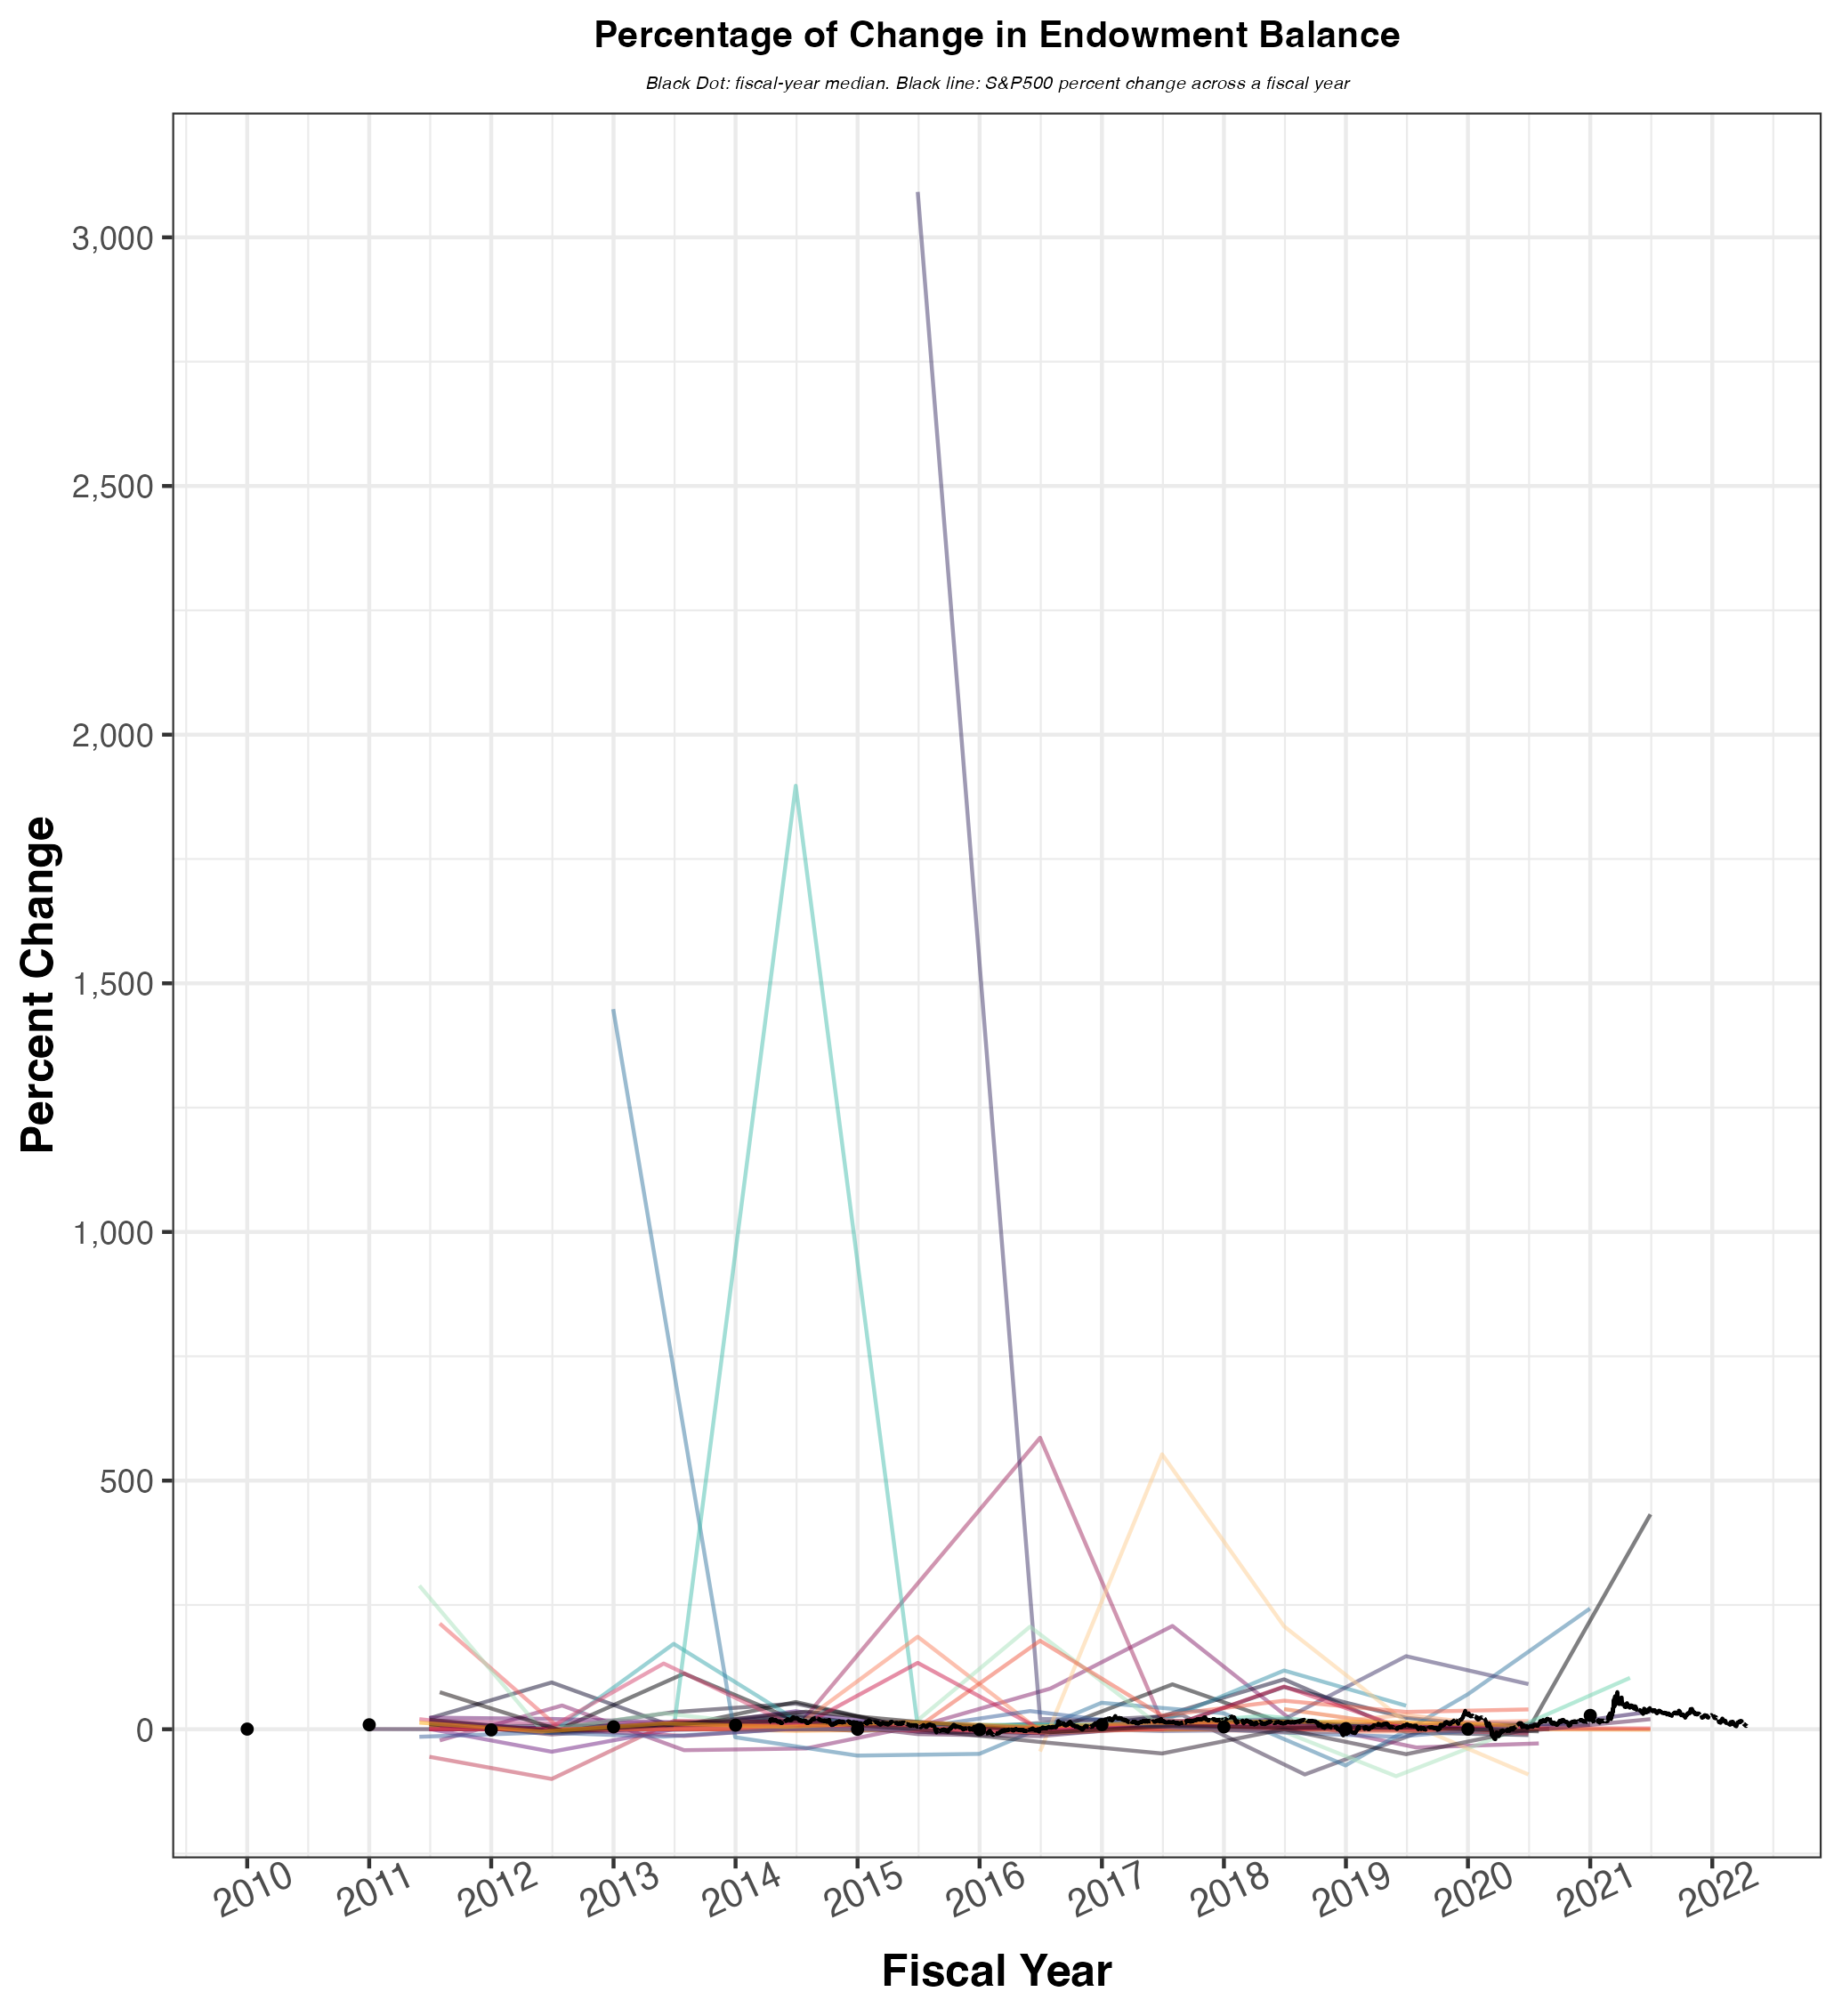
\includegraphics[width=0.8\linewidth,]{../images/pc_endow} \caption{\label{fig:perc-change-endow-all} Percent change in endowment balance over time, including the full range of percent changes, revealing several clear outliers.}\label{fig:unnamed-chunk-6}
\end{figure}

\begin{figure}[H]
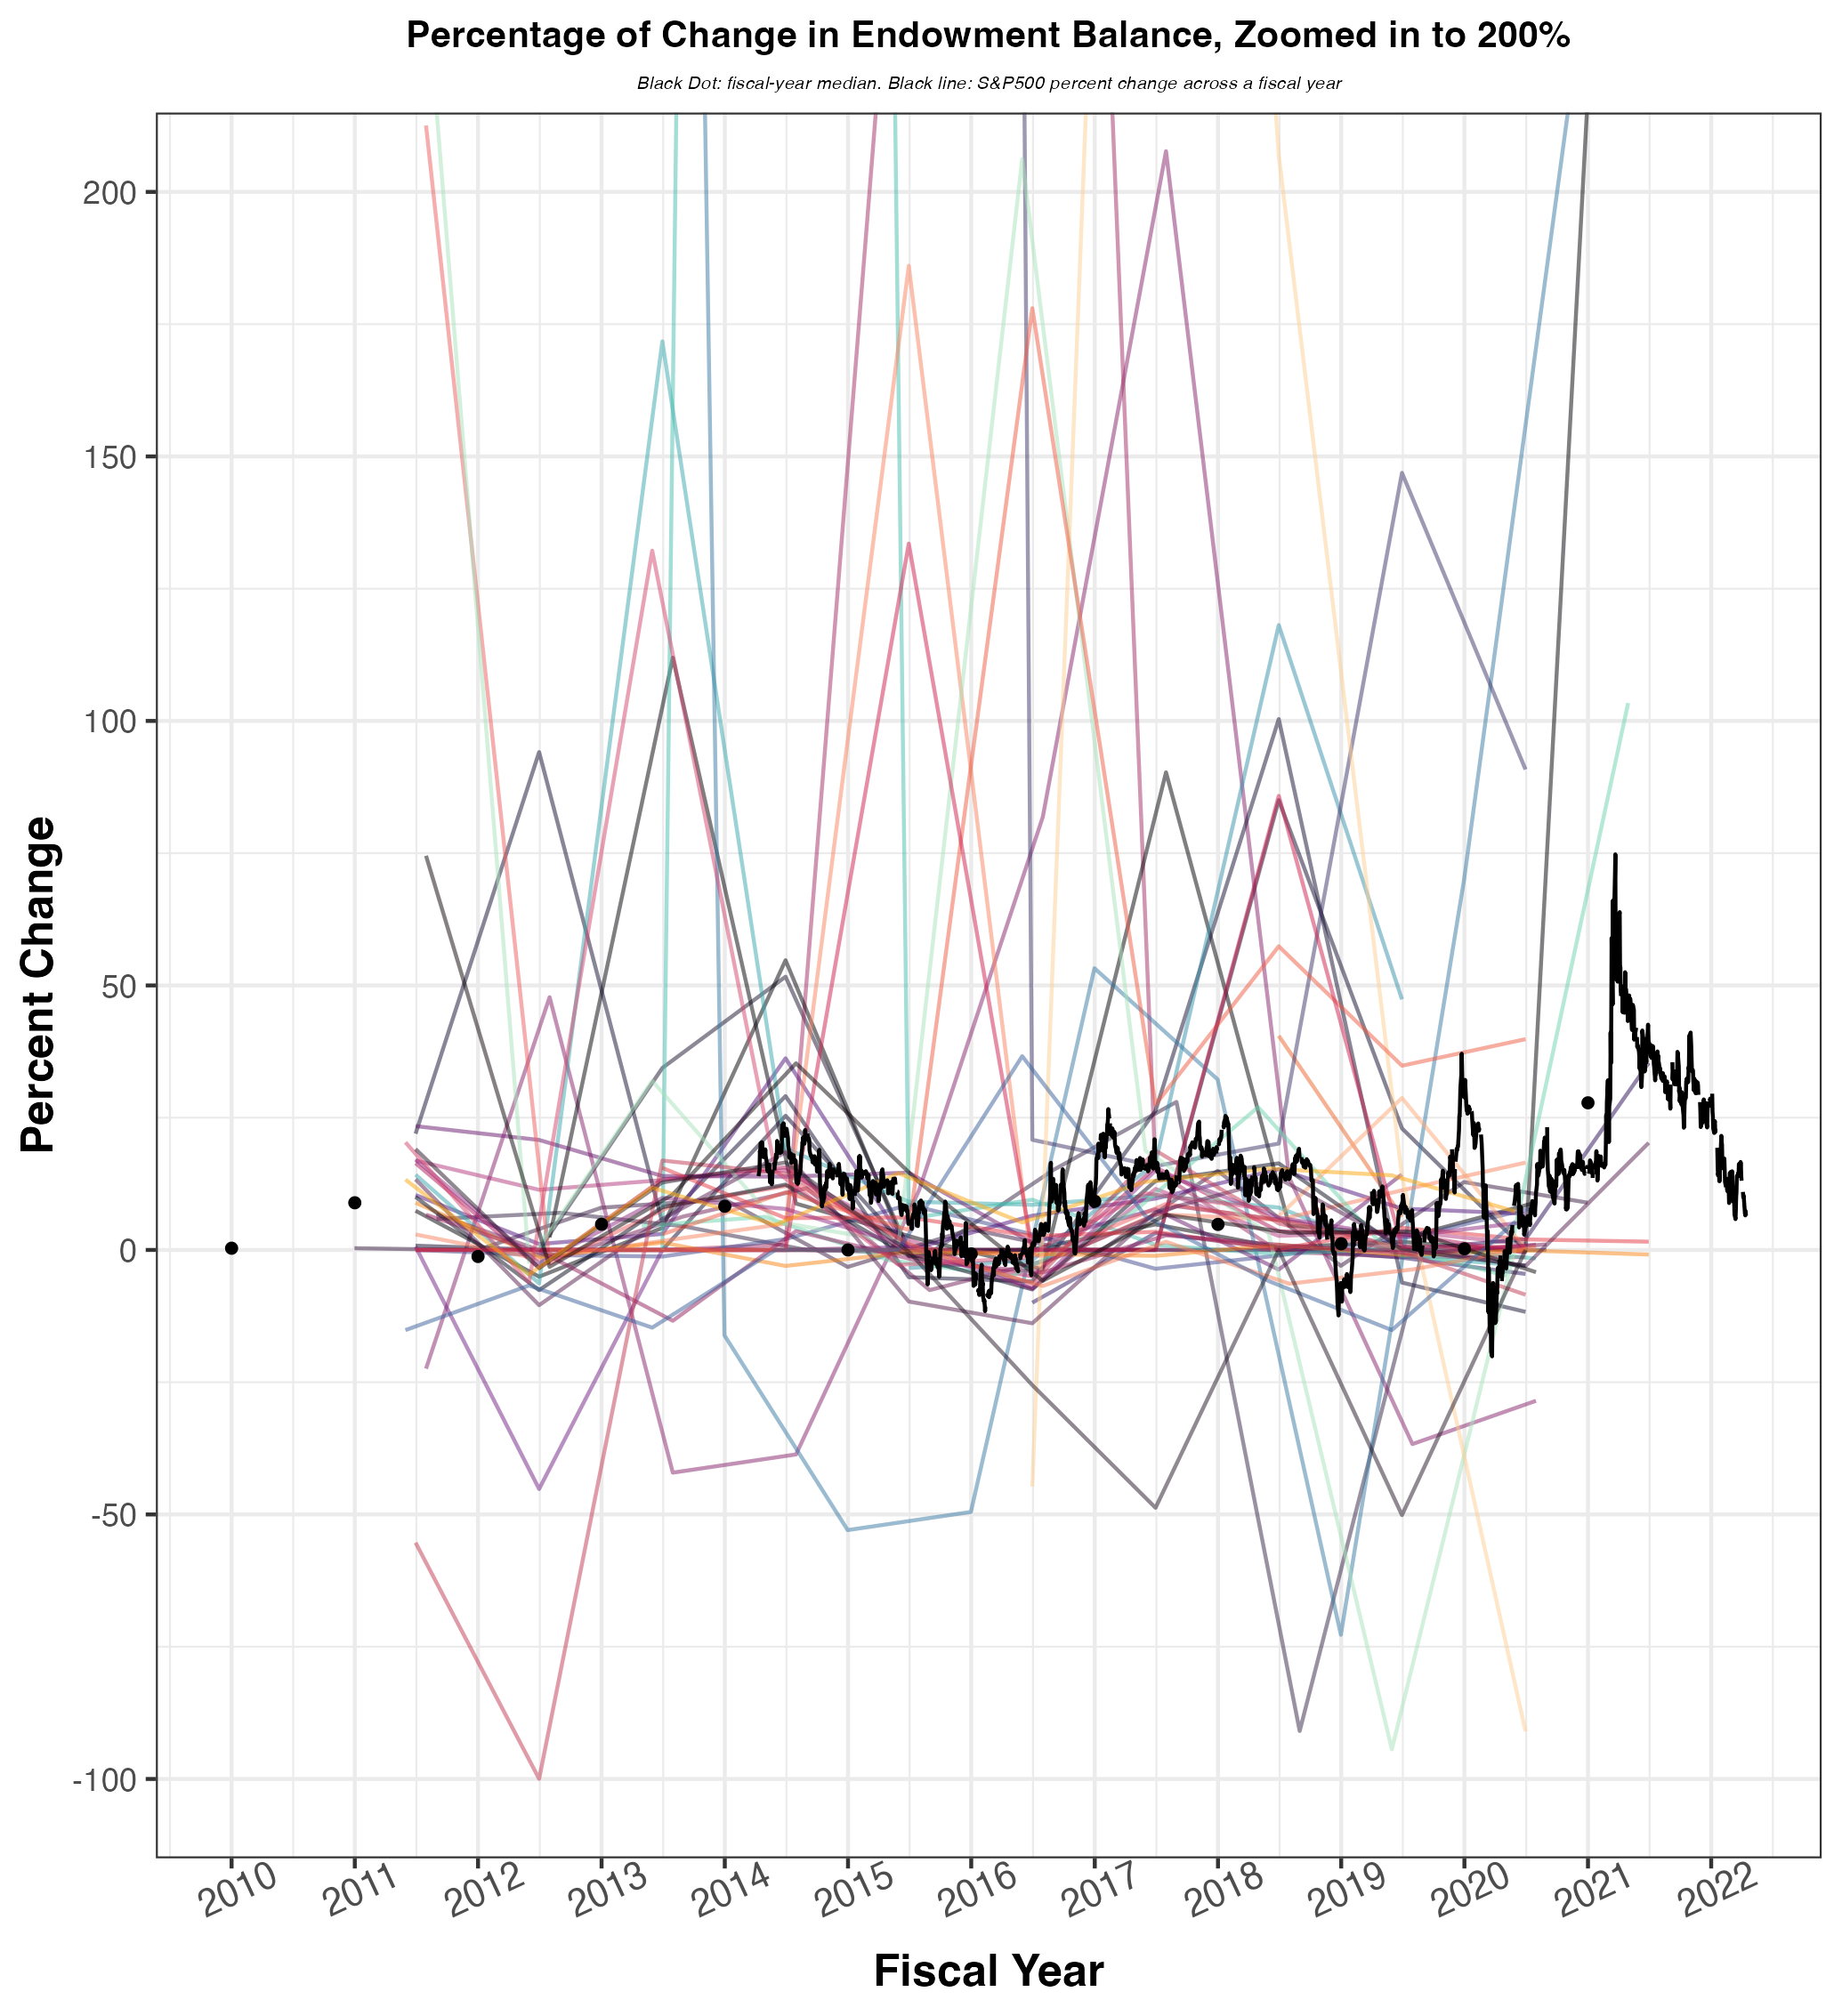
\includegraphics[width=0.8\linewidth,]{../images/pc_endow_zoom} \caption{\label{fig:perc-change-endow} Percent change in endowment balance over time, restricting the range to -200 percent to 200 percent to remove outliers than reduce our ability to see trends for the majority of companies.}\label{fig:unnamed-chunk-7}
\end{figure}

\begin{figure}[H]
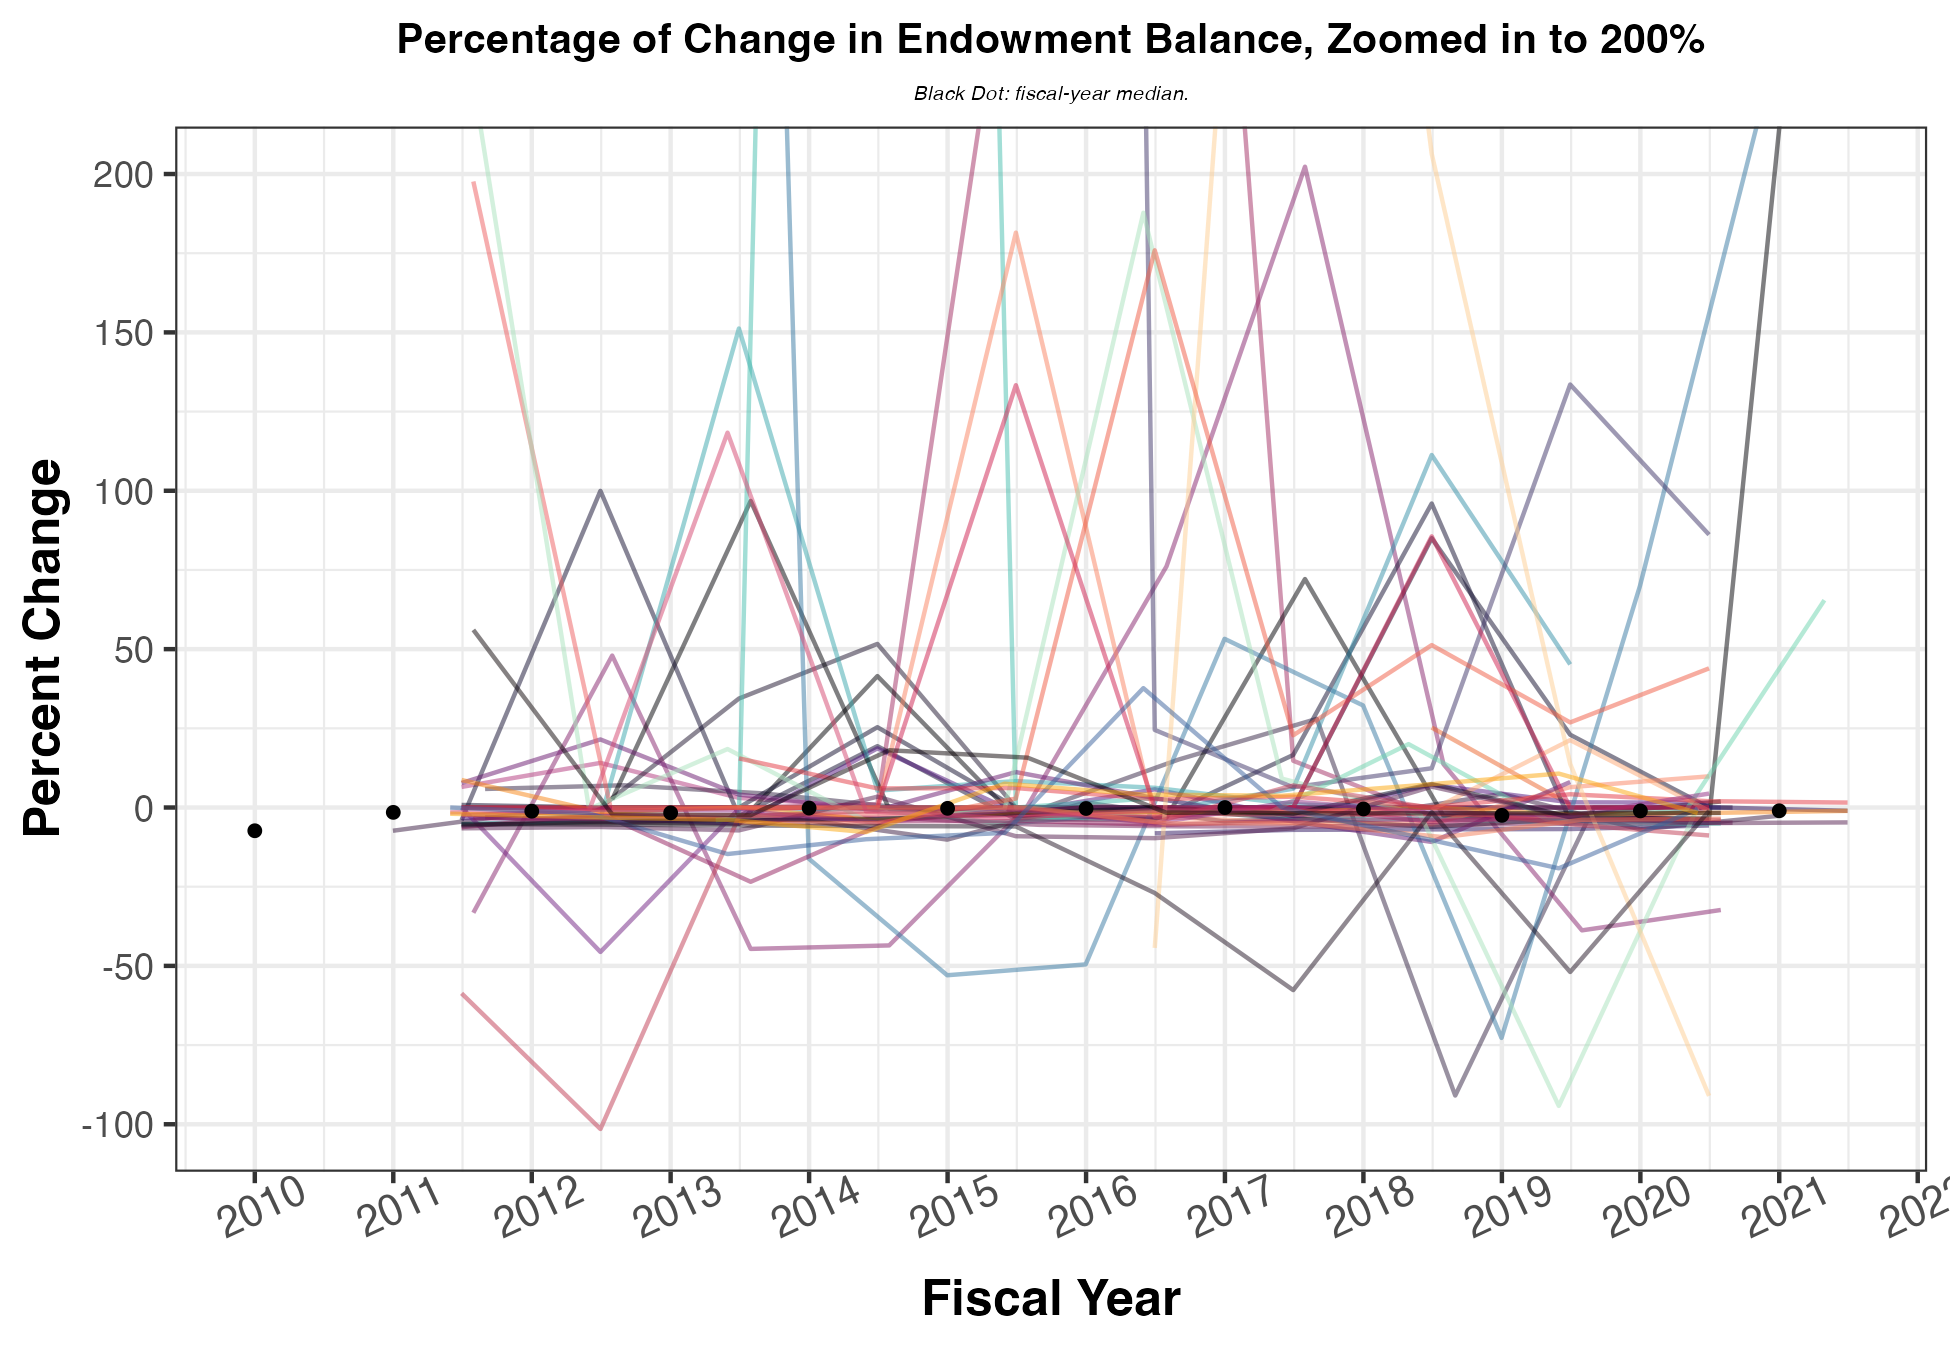
\includegraphics[width=0.8\linewidth,]{../images/pc_endow_flat} \caption{\label{fig:flat} Adjusting for investment earnings or losses when computing the endowment percent changes flattens the trends observable when using the unadjusted endowment values.}\label{fig:flat}
\end{figure}

Examining particular companies (Figure \ref{fig:below-40}), it is
apparent that eight companies reduce their endowment by over 40\%
(e.g.~Percent Change lower than -40\%) across multiple years. There are
eight companies that do so (Table 4) Aspen Santa Fe Ballet, Atlanta
Ballet, First State Ballet Theatre, Nashville Ballet, Orlando Ballet,
San Francisco Ballet, and The Washington Ballet. Some of these companies
reduce their endowments by over 40\% multiple times. While it is not
certain why more companies have such severe reductions in endowment
balance, reductions can indicate a variety of situations for a company,
such as: dispersing their funds into a new fiscal entity\footnote{Aspen
  Santa Fe Ballet transferred most of their endowment into Aspen Santa
  Fe Ballet Endowment Inc in 2018; see the note on Aspen Santa Fe in the
  \protect\hyperlink{asfb}{previous section}.}, struggling financially
in a given fiscal year, spending newly-unrestricted funds, or purchasing
large items such as a building. Few companies severely reduce their
endowment, thus the majority of US dance companies with endowments are
able to maintain their savings and receive income from their endowments.

\begin{figure}[H]
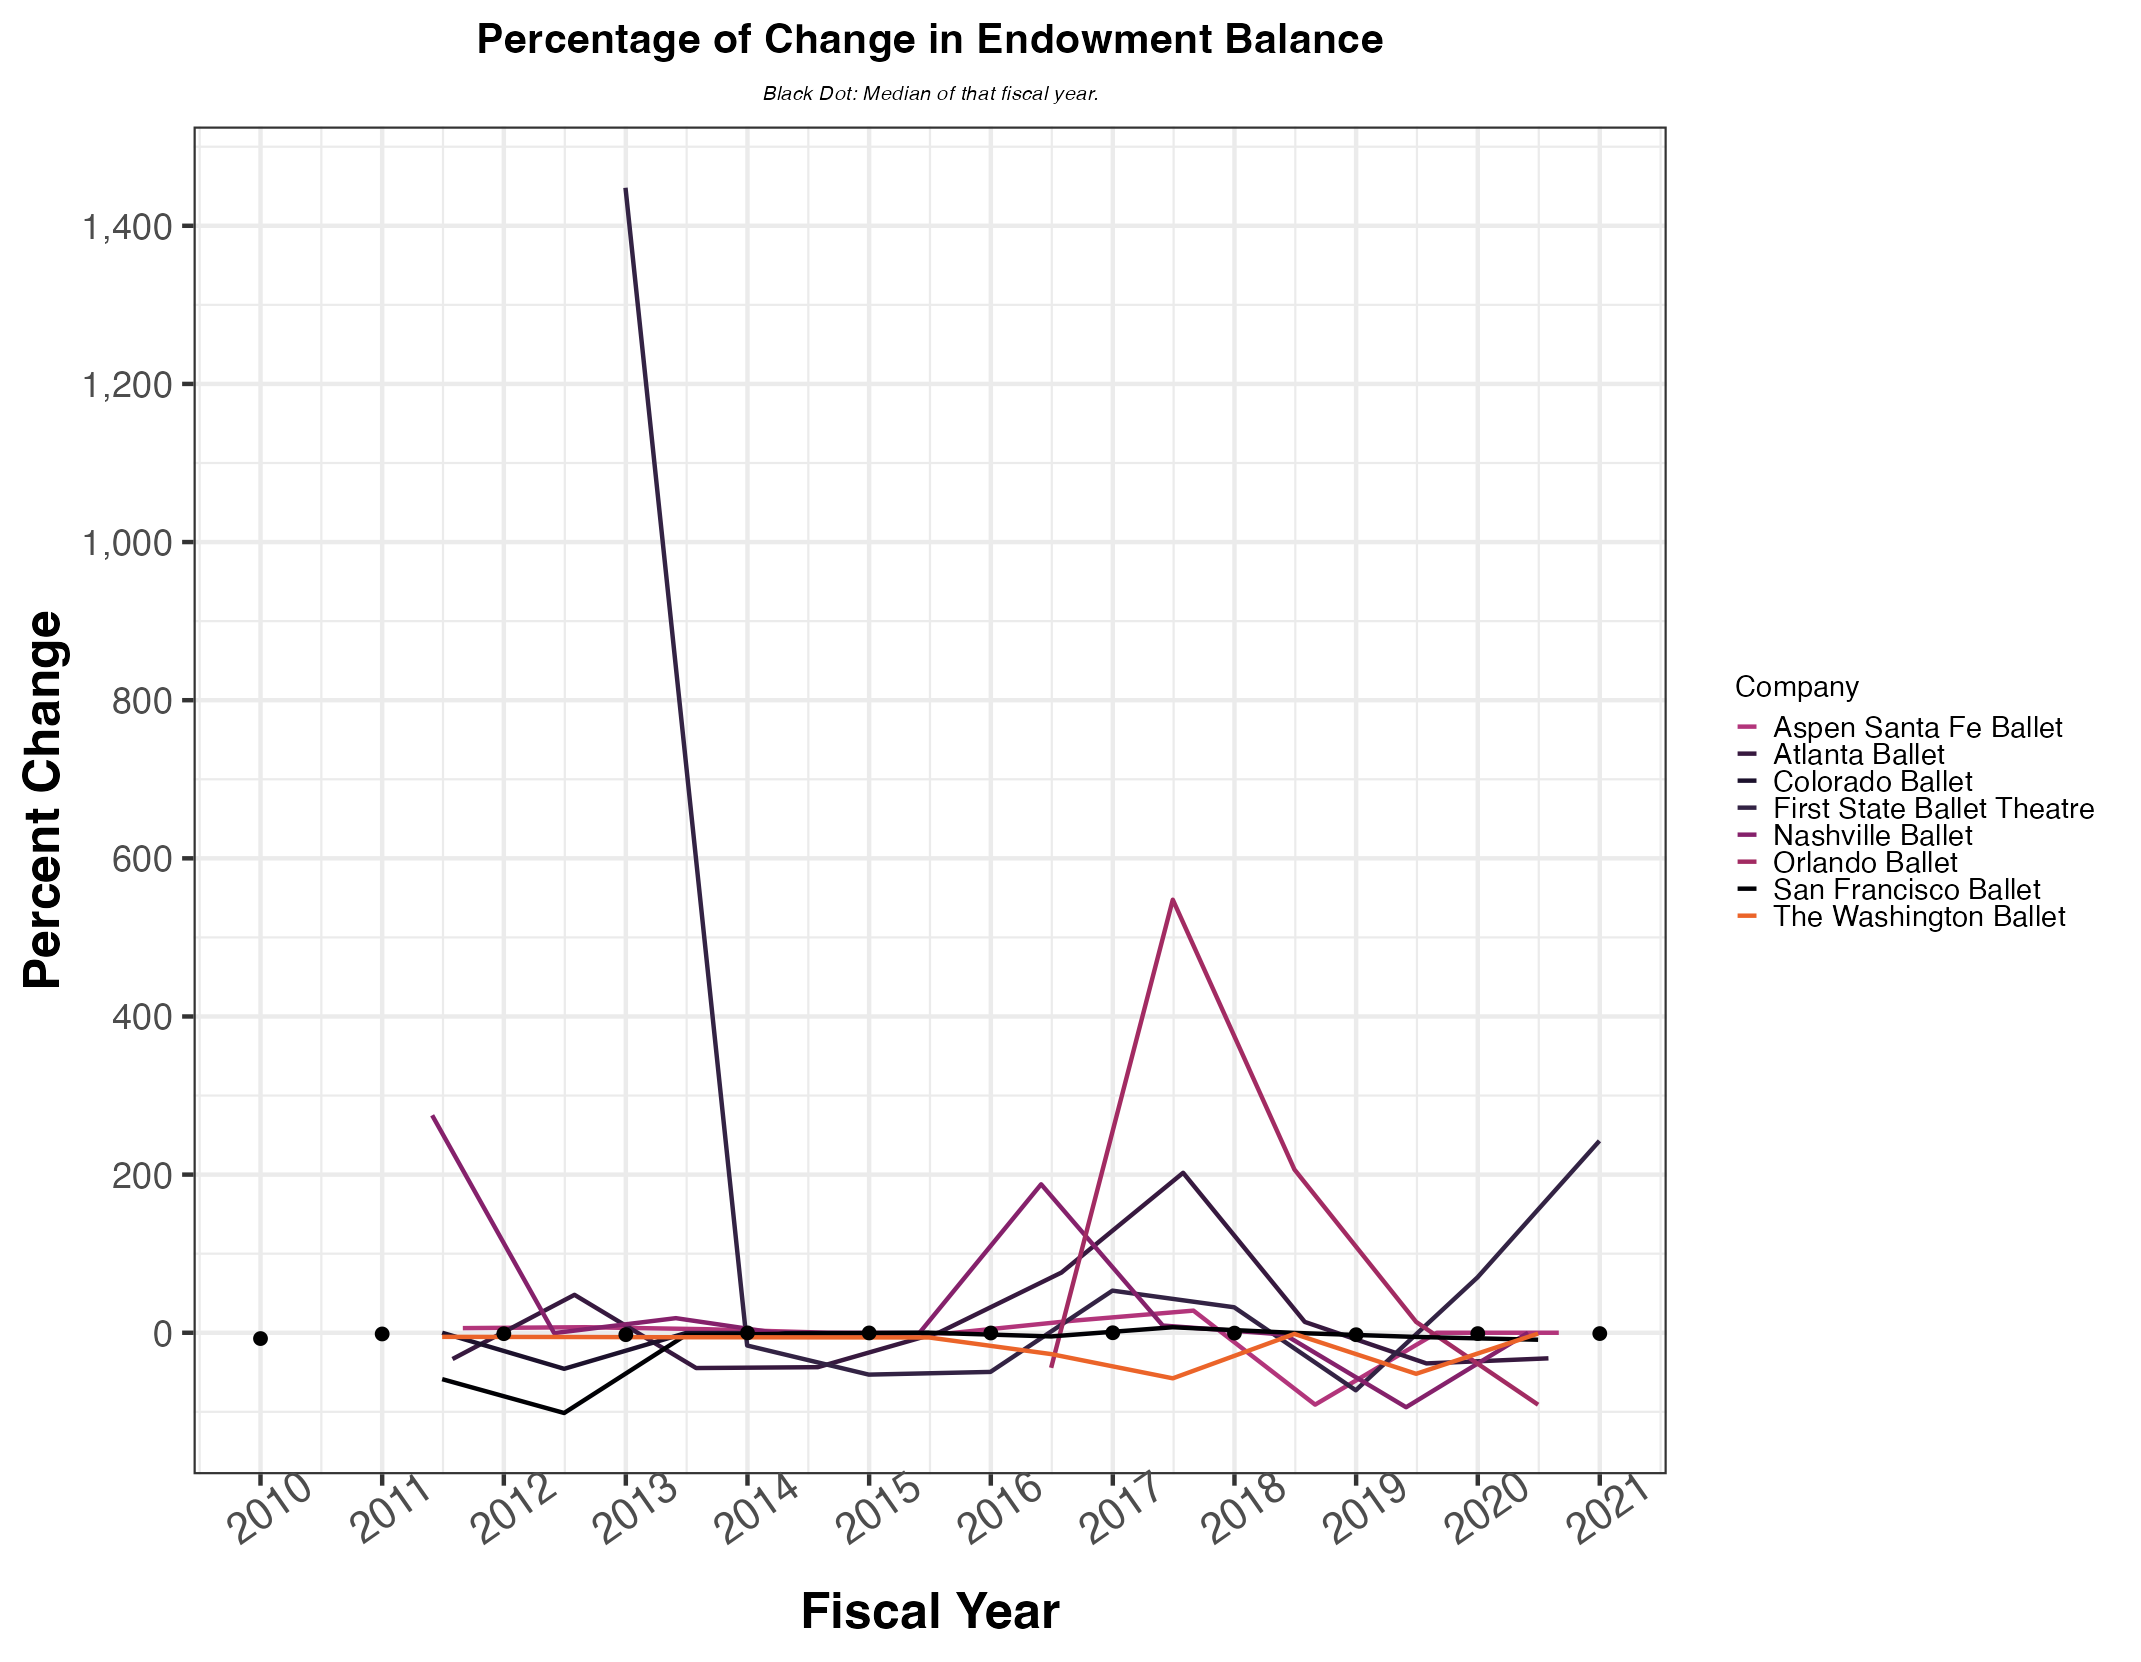
\includegraphics[width=1\linewidth,]{../images/pc_below_40} \caption{\label{fig:below-40} Companies that reduce their endowment by over 40 percent.}\label{fig:unnamed-chunk-8}
\end{figure}

\begin{table}[!h]

\caption{Endowment Percent Change Dropping Below 40 Percent Of Beginning Year balance}
\centering
\begin{tabular}[t]{lrrrr}
\toprule
Company Name & Percent Change & Beginning Balance & End Balance & Fiscal Year\\
\midrule
Aspen Santa Fe Ballet & -90.9 & 6065013 & 550000 & 2018\\
\addlinespace
Atlanta Ballet & -43.5 & 1706513 & 1046921 & 2014\\
\addlinespace
Atlanta Ballet & -44.6 & 2947203 & 1706513 & 2013\\
\addlinespace
Colorado Ballet & -45.6 & 182437 & 100000 & 2012\\
\addlinespace
First State Ballet Theatre & -72.7 & 36693 & 10000 & 2018\\
\addlinespace
First State Ballet Theatre & -49.5 & 35876 & 18107 & 2015\\
\addlinespace
First State Ballet Theatre & -53.0 & 76261 & 35876 & 2014\\
\addlinespace
Nashville Ballet & -94.2 & 1095624 & 61350 & 2019\\
\addlinespace
Orlando Ballet & -91.0 & 7732855 & 696082 & 2020\\
\addlinespace
Orlando Ballet & -44.3 & 613186 & 338943 & 2016\\
\addlinespace
San Francisco Ballet & -101.5 & 1035814 & 174 & 2012\\
\addlinespace
San Francisco Ballet & -58.7 & 2318646 & 1035814 & 2011\\
\addlinespace
The Washington Ballet & -51.9 & 621423 & 310000 & 2019\\
\addlinespace
The Washington Ballet & -57.6 & 1212247 & 621423 & 2017\\
\bottomrule
\end{tabular}
\end{table}

Additionally, eight companies increased their endowment by over 200\%
(percent Change higher than 200\%) across multiple years, which means
they at minimum tripled their endowment (\ref{fig:above-200}). These
eight companies are Atlanta Ballet, Ballet Arizona, Ballet Hispánico,
First State Ballet Theatre, Fort Wayne Ballet, Joffrey Ballet, Nashville
Ballet, and Orlando Ballet. Such dramatic increases are potentially
indicative of large donations, liquidation of assets such as buildings,
or aggregation of funds from separate endowment accounts.

\begin{figure}[H]
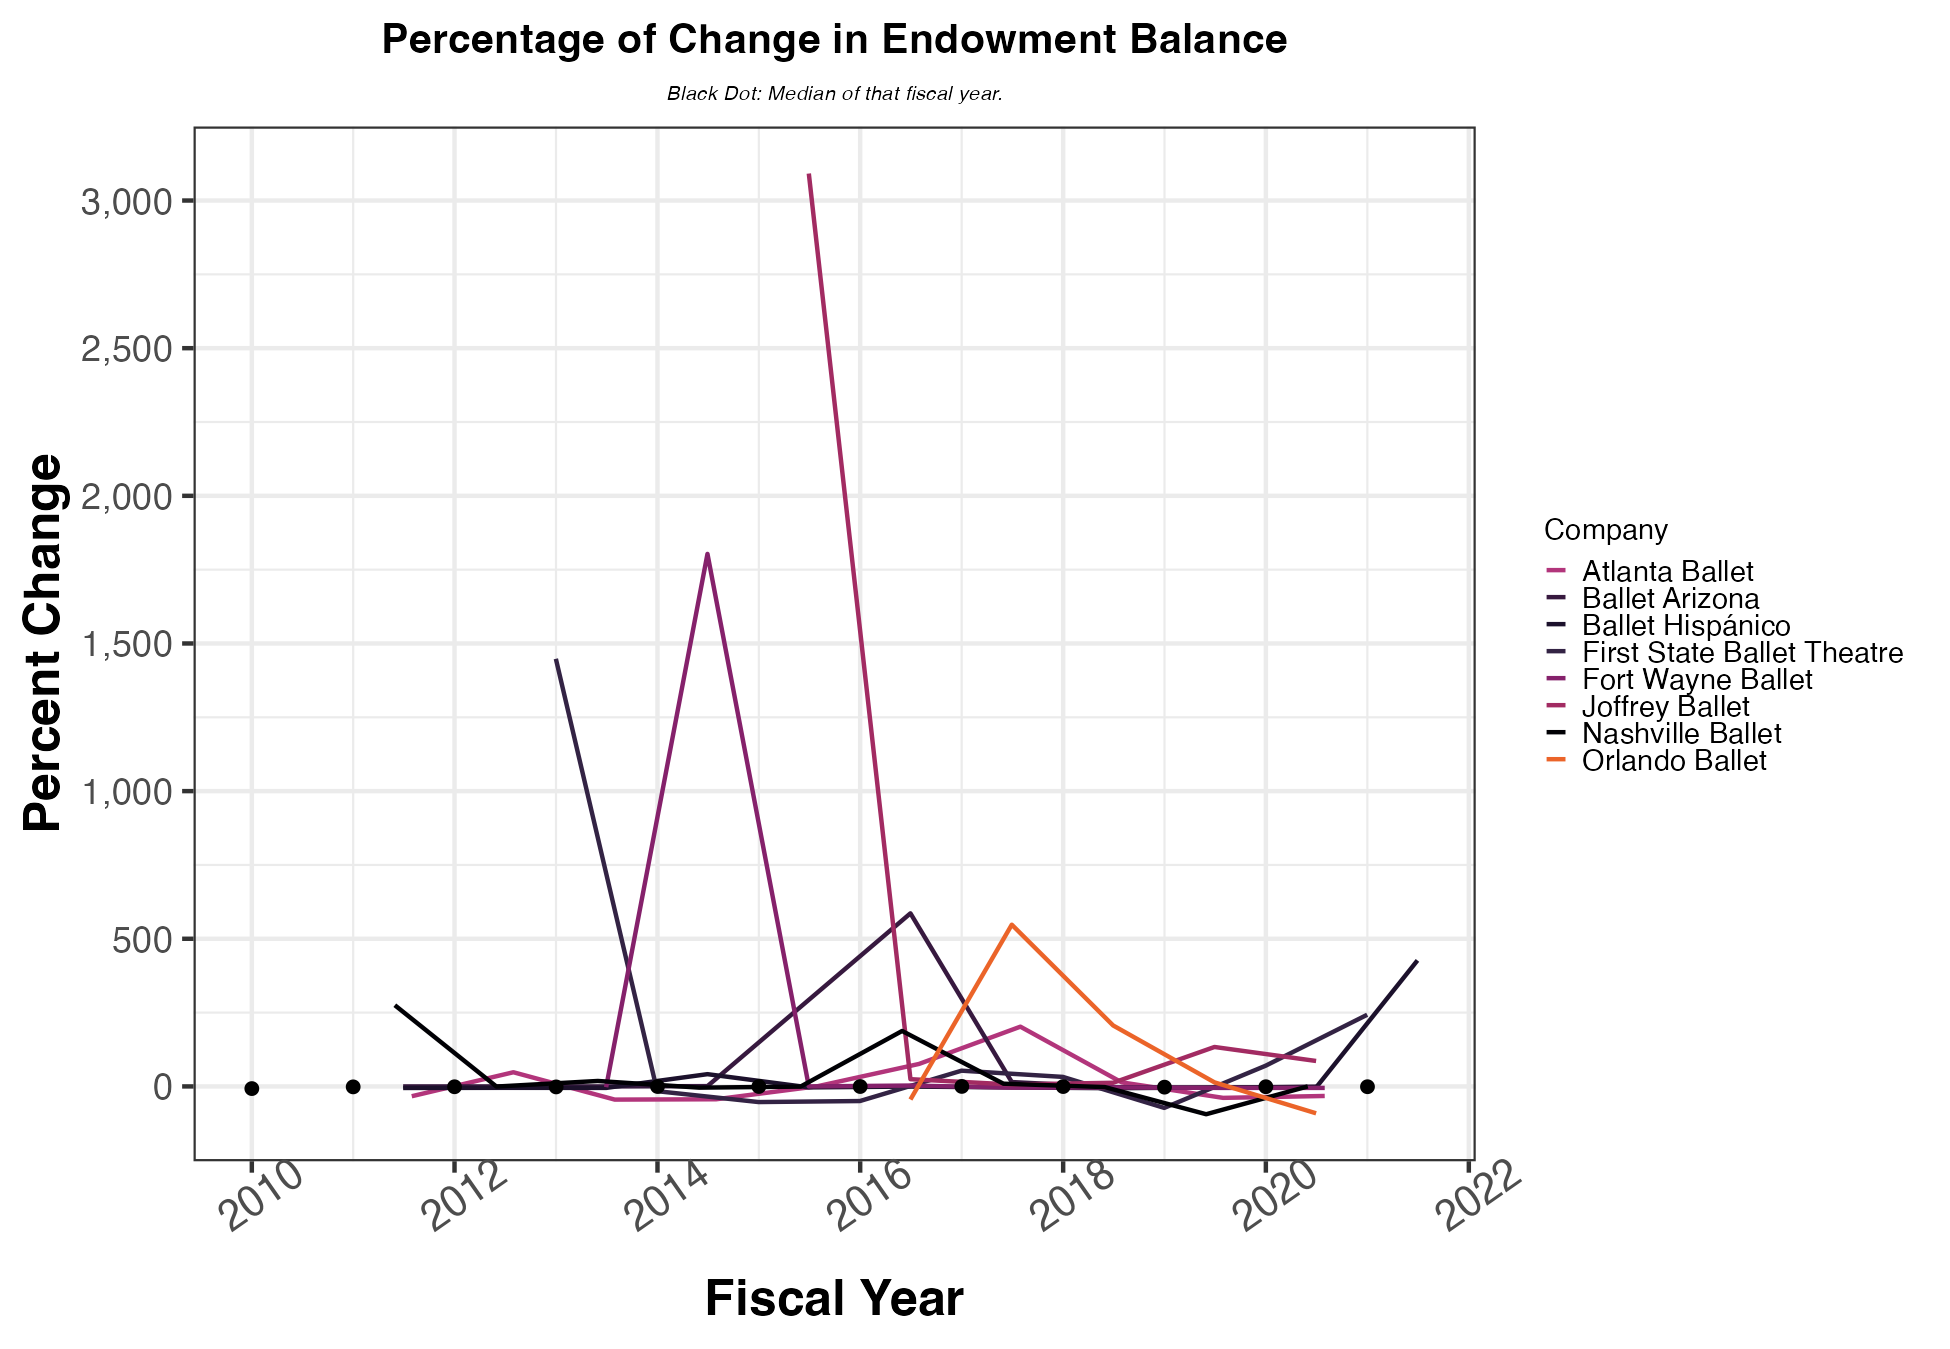
\includegraphics[width=0.9\linewidth,]{../images/pc_above_200} \caption{\label{fig:above-200} Annual percent change for companies that increased their endowment over 200 percent.}\label{fig:unnamed-chunk-9}
\end{figure}

\begin{table}

\caption{Endowment Percent Change Increasing Beyond 200 Percent Of Beginning Year Balance}
\centering
\begin{tabular}[t]{lrrrr}
\toprule
Company Name & Percent Change & Beginning Balance & End Balance & Fiscal Year\\
\midrule
Atlanta Ballet & 202.3 & 2119967 & 6523144 & 2017\\
\addlinespace
Ballet Arizona & 586.1 & 601399 & 4126424 & 2016\\
\addlinespace
Ballet Hispánico & 426.8 & 1405952 & 7481852 & 2021\\
\addlinespace
First State Ballet Theatre & 242.7 & 16999 & 58253 & 2020\\
\addlinespace
First State Ballet Theatre & 242.7 & 16999 & 58253 & 2020\\
\addlinespace
First State Ballet Theatre & 1448.1 & 5874 & 90934 & 2012\\
\addlinespace
Fort Wayne Ballet & 1803.3 & 60137 & 1201082 & 2014\\
\addlinespace
Joffrey Ballet & 3091.4 & 35600 & 1136139 & 2015\\
\addlinespace
Nashville Ballet & 275.0 & 54543 & 212030 & 2011\\
\addlinespace
Orlando Ballet & 206.4 & 2212808 & 6791249 & 2018\\
\addlinespace
Orlando Ballet & 547.7 & 338943 & 2212808 & 2017\\
\bottomrule
\end{tabular}
\end{table}

To examine the behavior of endowments, each company was ranked by its
consistency over time. Consistency is defined by ranking companies by
their standard deviation of a company's percent change across all years
on file. The smaller the standard deviation, the more consistent the
company's endowment behavior was, thus the higher the rank. (Figure
\ref{fig:pc-consist}). Many companies that have consistent balances tend
to not make large adjustments to their percent change. Further,
consistency in endowment does not appear to be related to company size
(Figure \ref{fig:endo-size}), as measured by both the endowment total
balance and the number of employees.

\begin{figure}[H]
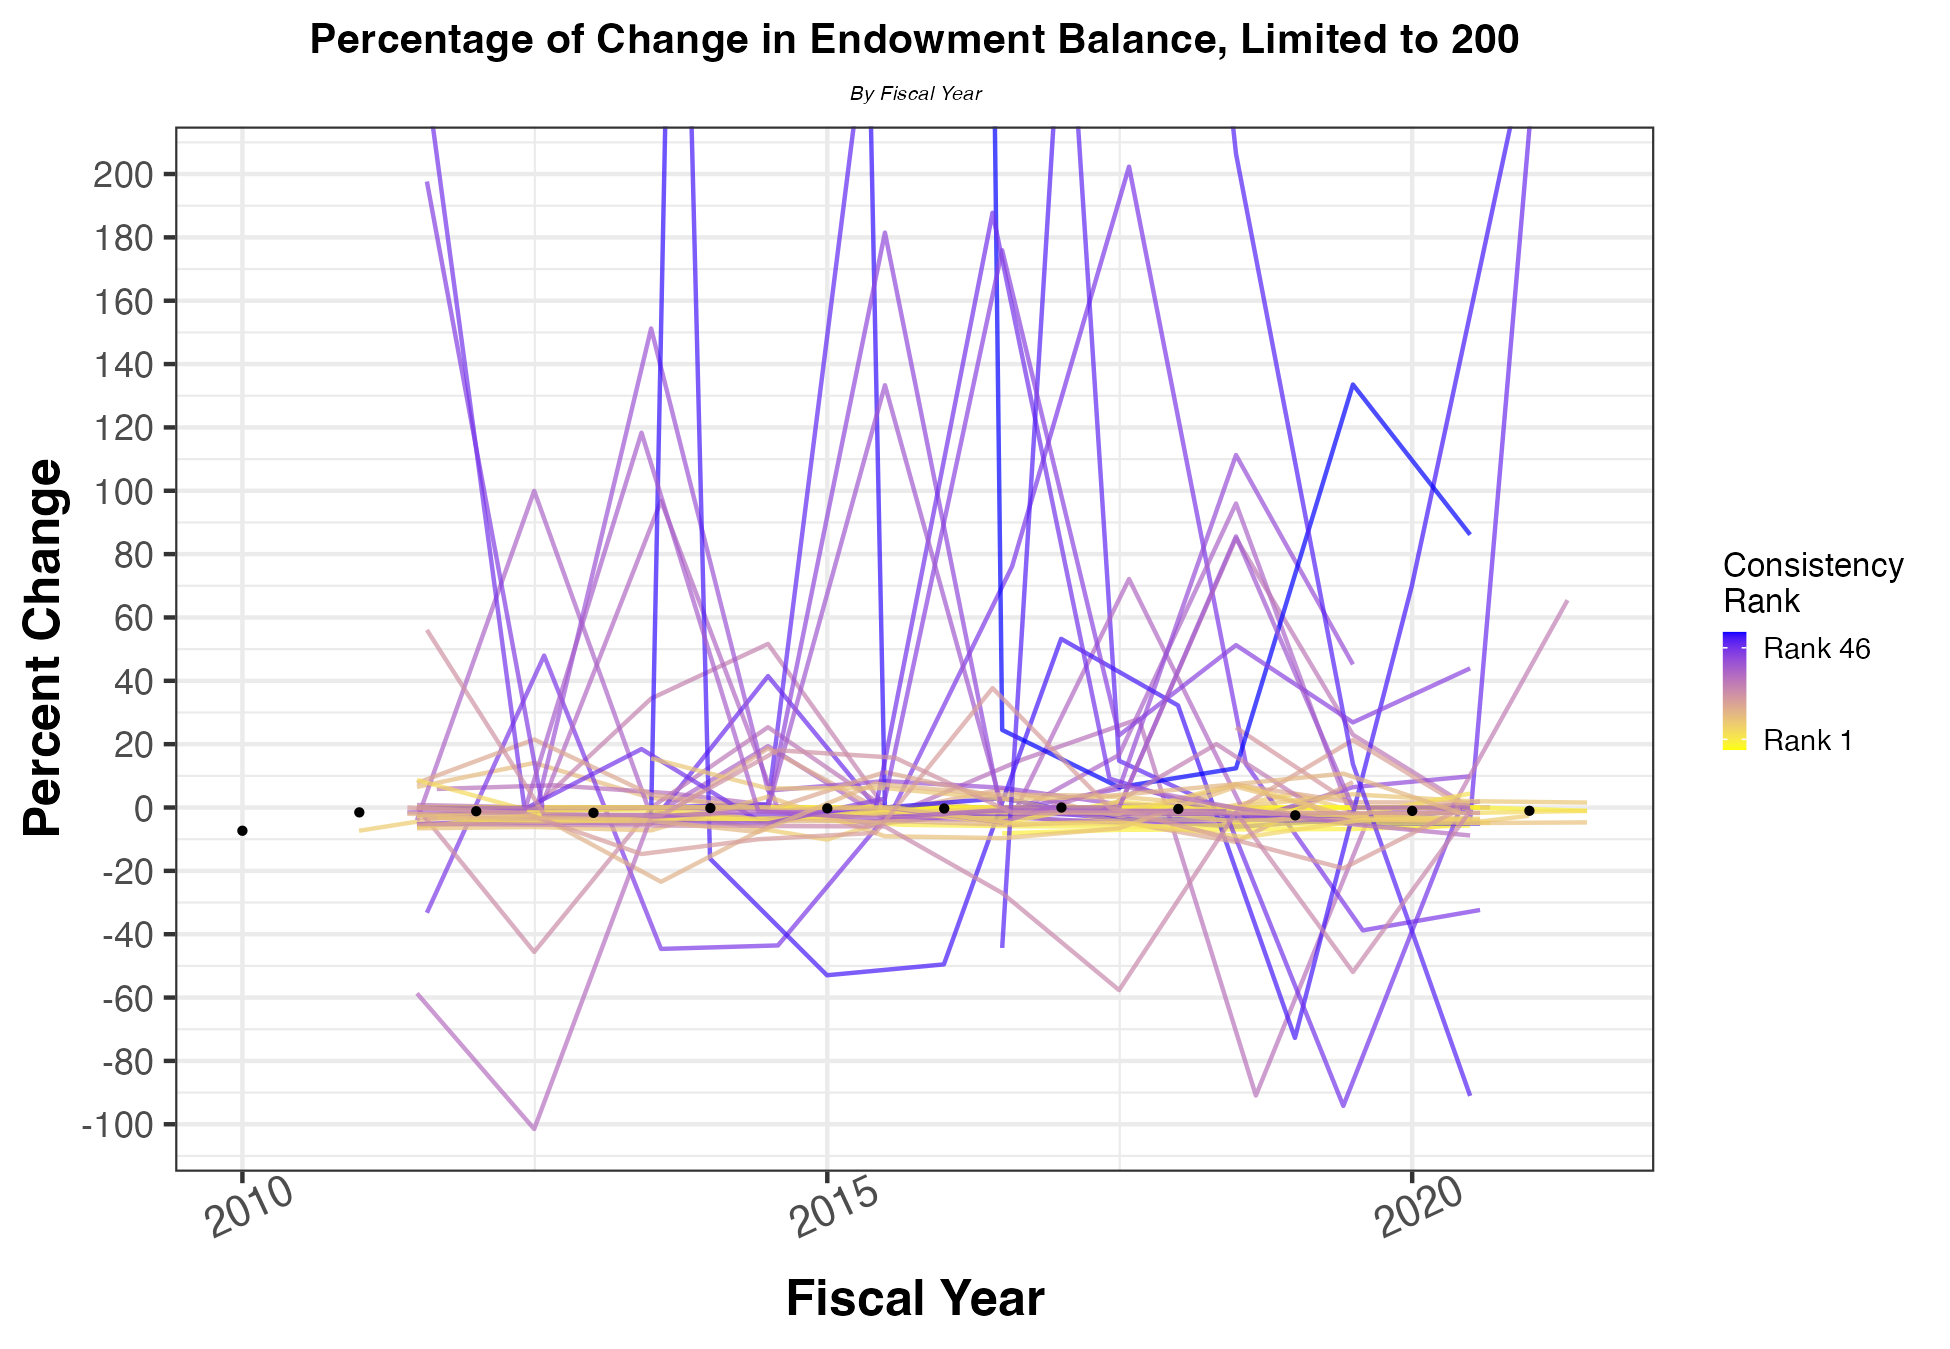
\includegraphics[width=0.9\linewidth,]{../images/pc_consist} \caption{\label{fig:pc-consist}}\label{fig:unnamed-chunk-10}
\end{figure}

\begin{figure}[H]
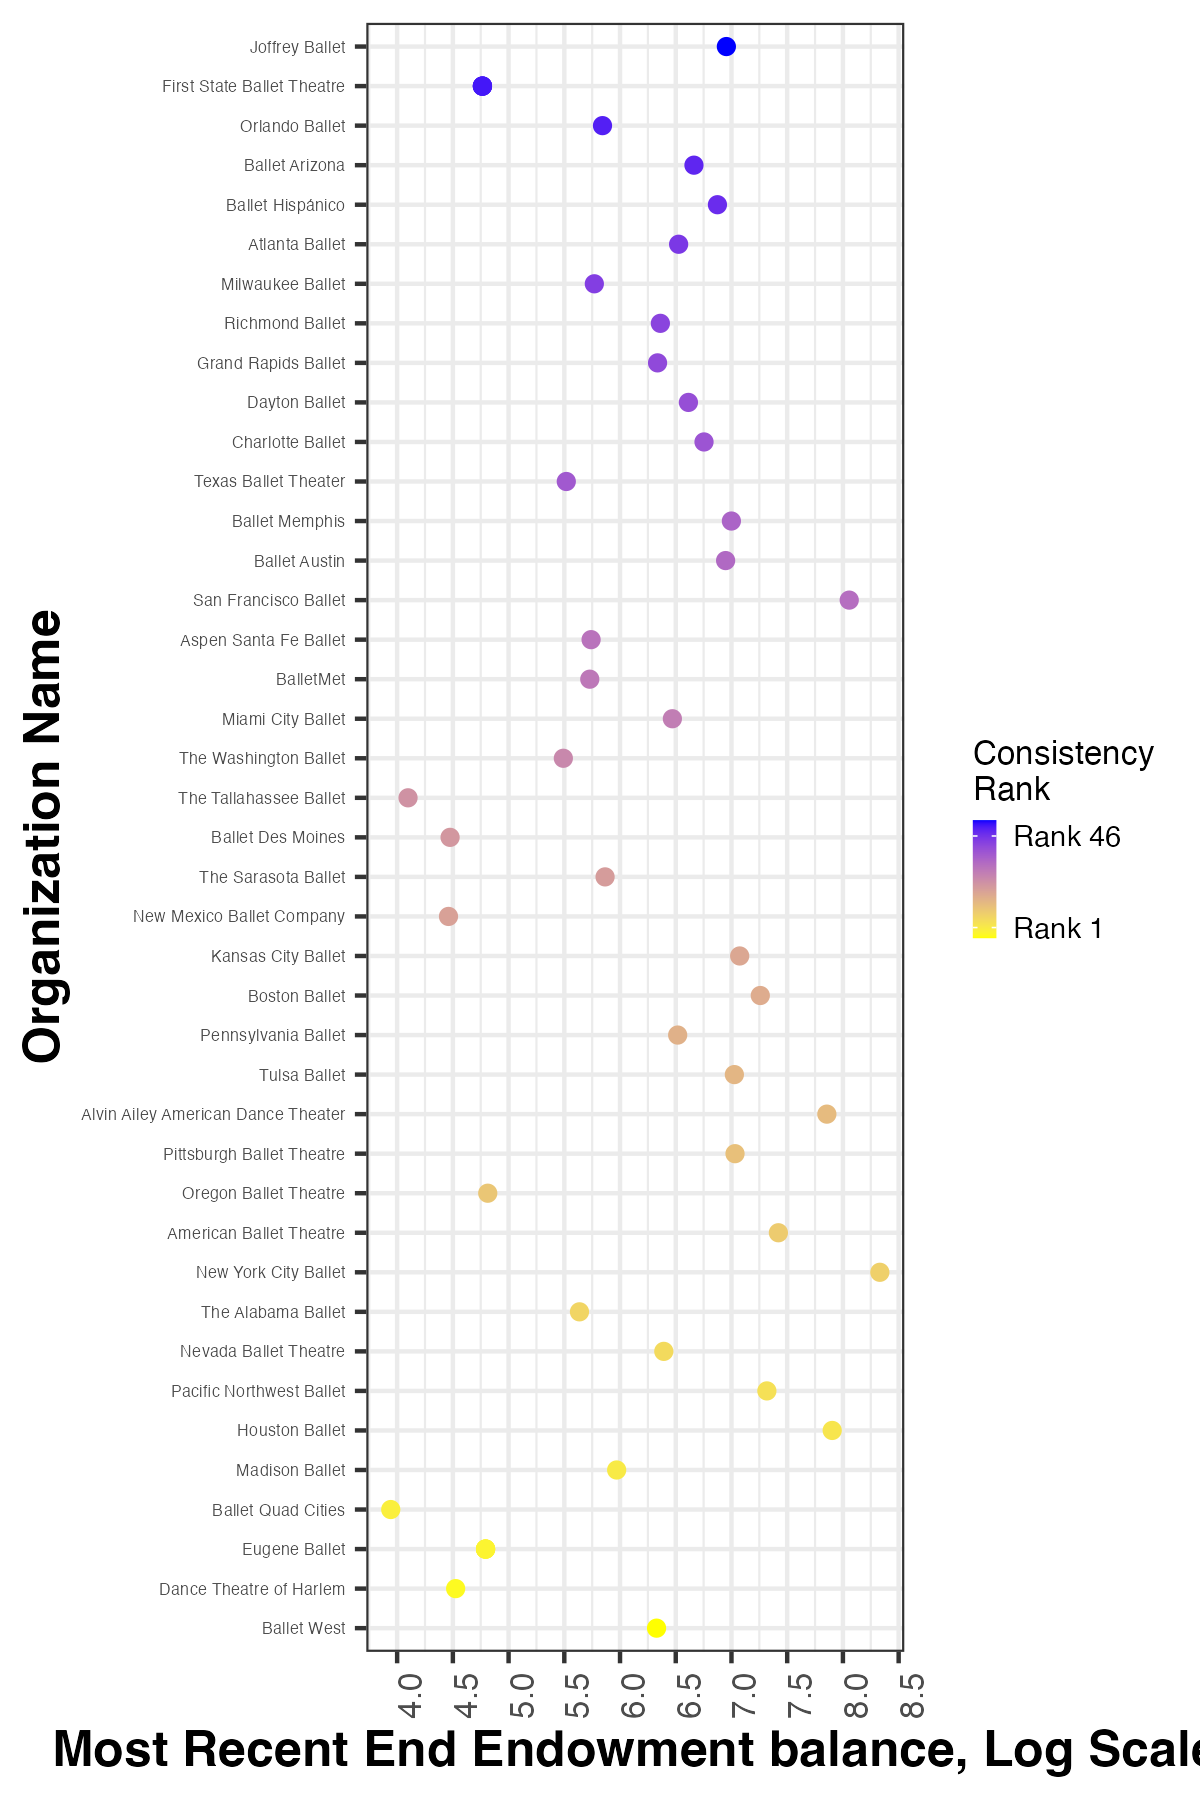
\includegraphics[width=0.5\linewidth,]{../images/consist_by_endo_size} 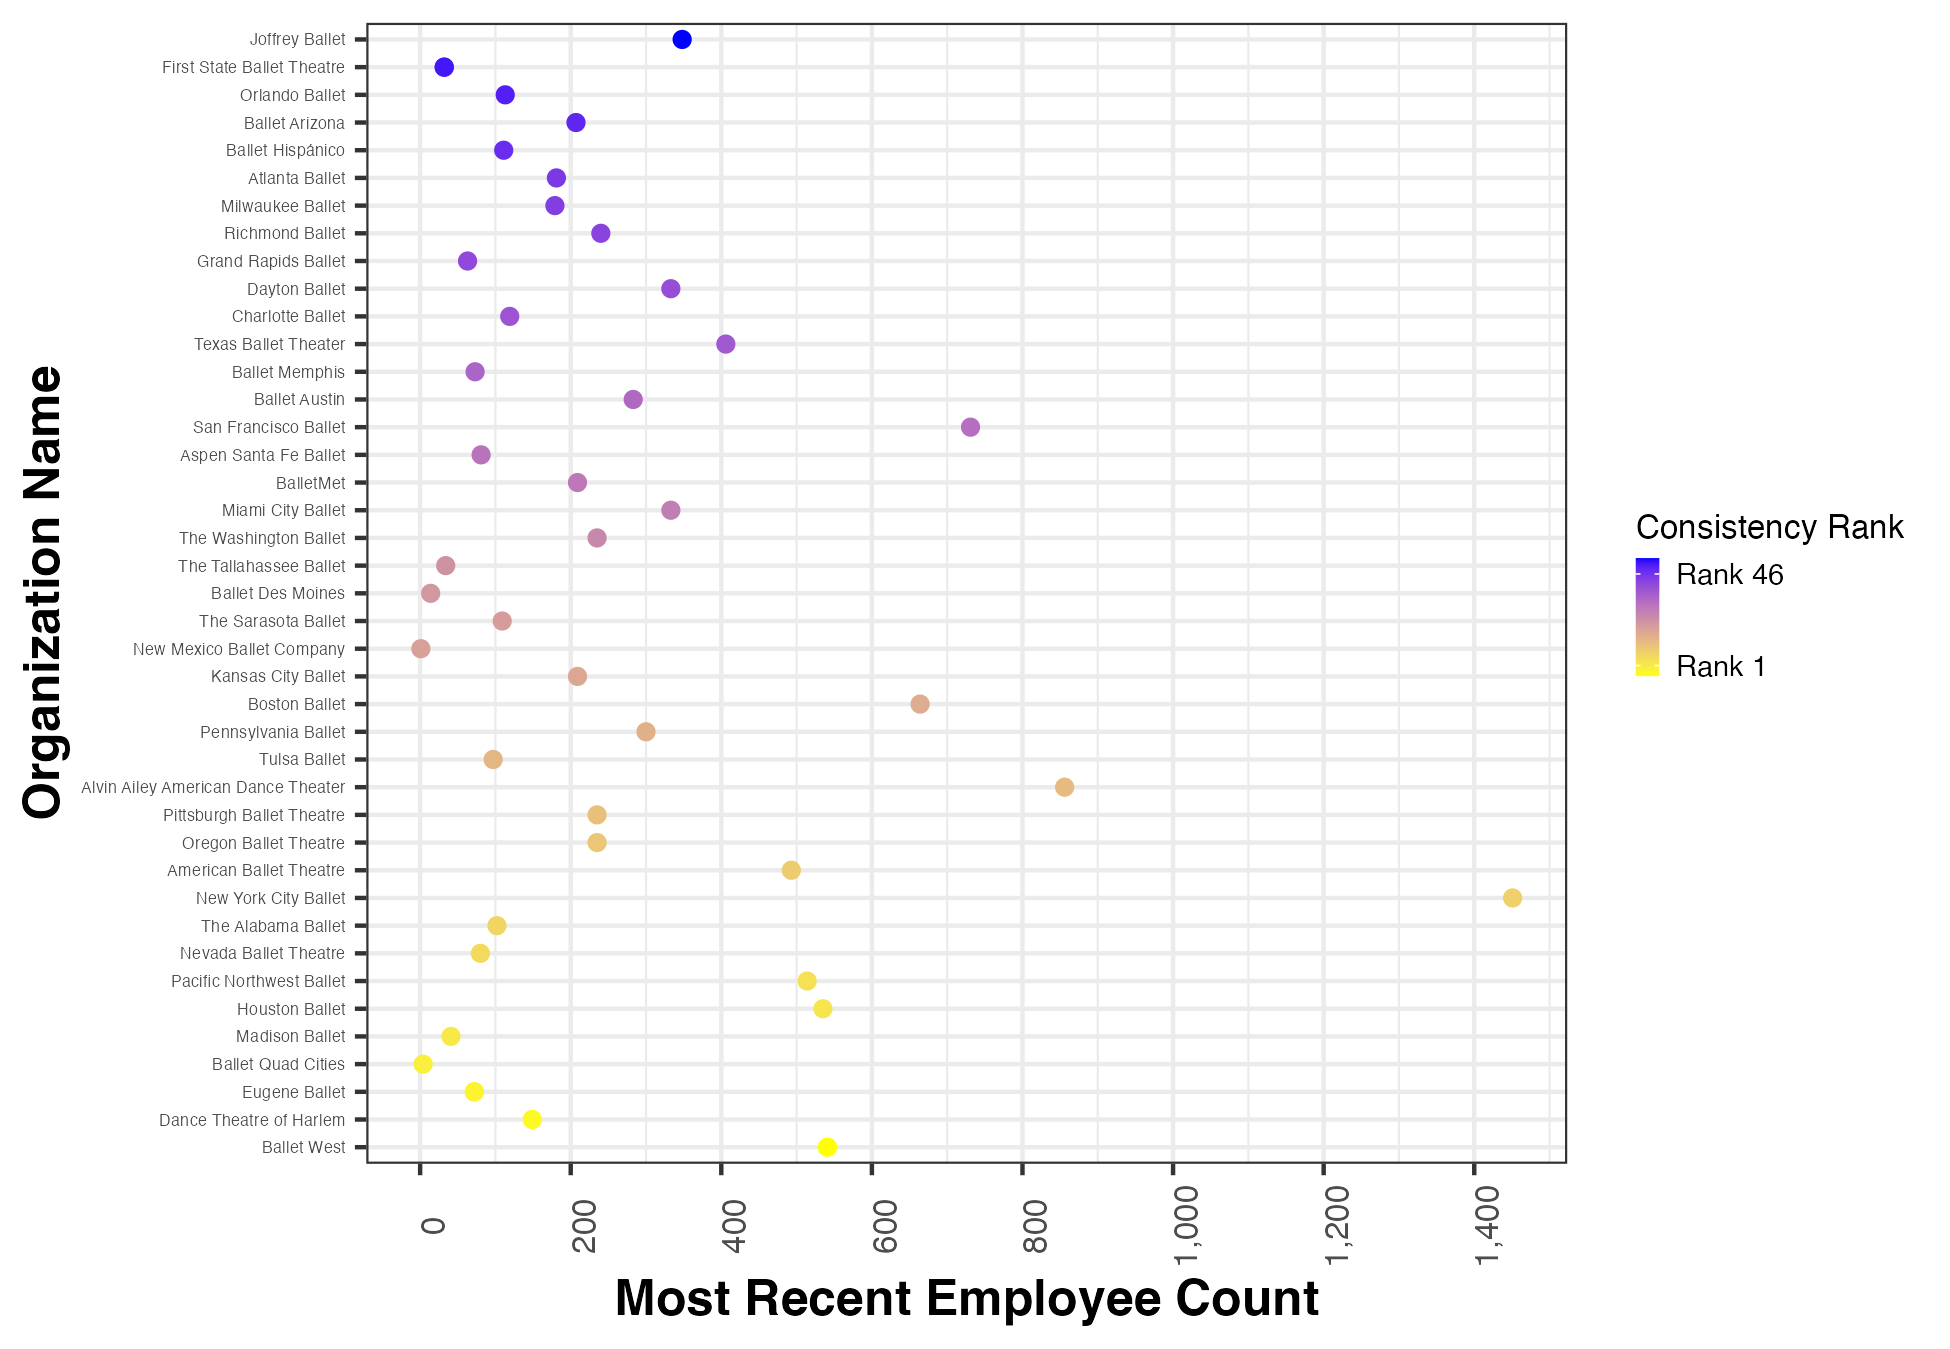
\includegraphics[width=0.5\linewidth,]{../images/consist_by_employ_count} \caption{\label{fig:endo-size}}\label{fig:unnamed-chunk-11}
\end{figure}

\hypertarget{endowment-time}{%
\subsubsection{Compound Annual Growth Rate}\label{endowment-time}}

The compound annual growth rate is a useful way to summarize the
performance of different endowments over the same time period since the
variability in annual growth rates can make it difficult to see broader
trends. One can think of this rate where, if the value grew by this same
rate each year, it would produce the end value at the end of the time
period considered.

When looking at the compound annual growth rate in this setting, it is
helpful to account for withdrawals and contributions to separate how
endowments are doing due to investment decisions versus how they change
due to large contributions or withdrawals.

The basic formula for the compound growth rate over \(t\) years is

\[{\text{Compound Annual Growth Rate} = \left( \frac{\text{End Value}}{\text{Beginning Value}}\right)^{\frac{1}{t}}-1}.\]

Withdrawals as reported on the 990 include other expenditures, grants
and scholarships, and administrative expenses.

This means it is possible to compute the withdrawals for any given year
and company as

\[\small{\text{Withdrawals} = \text{Other Expenditures} +\text{Administrative Expenses} +\text{Administrative Expenses} + \text{Grants and Scholarships}}.\]

To adjust for contributions and expenditures, the Compound Annual Growth
Rate is defined as
\[{\left( \frac{\text{End Value} + \sum_{i=1}^{t-1} \text{Withdrawals} - \sum_{i=1}^{t-1} \text{Contributions}  }{\text{Beginning Value}} \right)^{\frac{1}{t}}-1}.\]

Adding back the withdrawals and subtracting off the contributions
facilitates visualization of differences in endowments that are due
specifically to investment choices. Otherwise, it would not be possible
to tell whether a large increase in endowment funds in a particular year
was due to investment gains or a large contribution.

In Figure \ref{fig:compound-growth}, the compound growth rates of the
companies to the compound growth rate of the S\&P 500 over the same time
period are compared, where the S\&P 500 is used as a benchmark to
indicate how the stock market is doing overall. Variations in the S\&P
500 across companies for a given time interval are due to differences in
their fiscal years. While Ballet Arizona and San Francisco have enormous
differences when considering the time intervals 2011 to 2020 and 2015 to
2020, it is unclear whether these changes are truly this large in
magnitude or if the differences are due to discrepancies in reporting.
Although the capstone team reached out to both companies to clarify
discrepancies in the early years, the capstone team received no reply.

A substantial proportion (about 40\% of the companies for the 2011-2020
time period, and about 50\% of companies for the 2015-2020 and 2017-2020
time periods) had a compound annual growth rate of less than 5\%. The
same concept is clear at a more granular level considering the annual
growth rates in Figure \ref{fig:annual-growth-endowment}.

\begin{figure}[H]
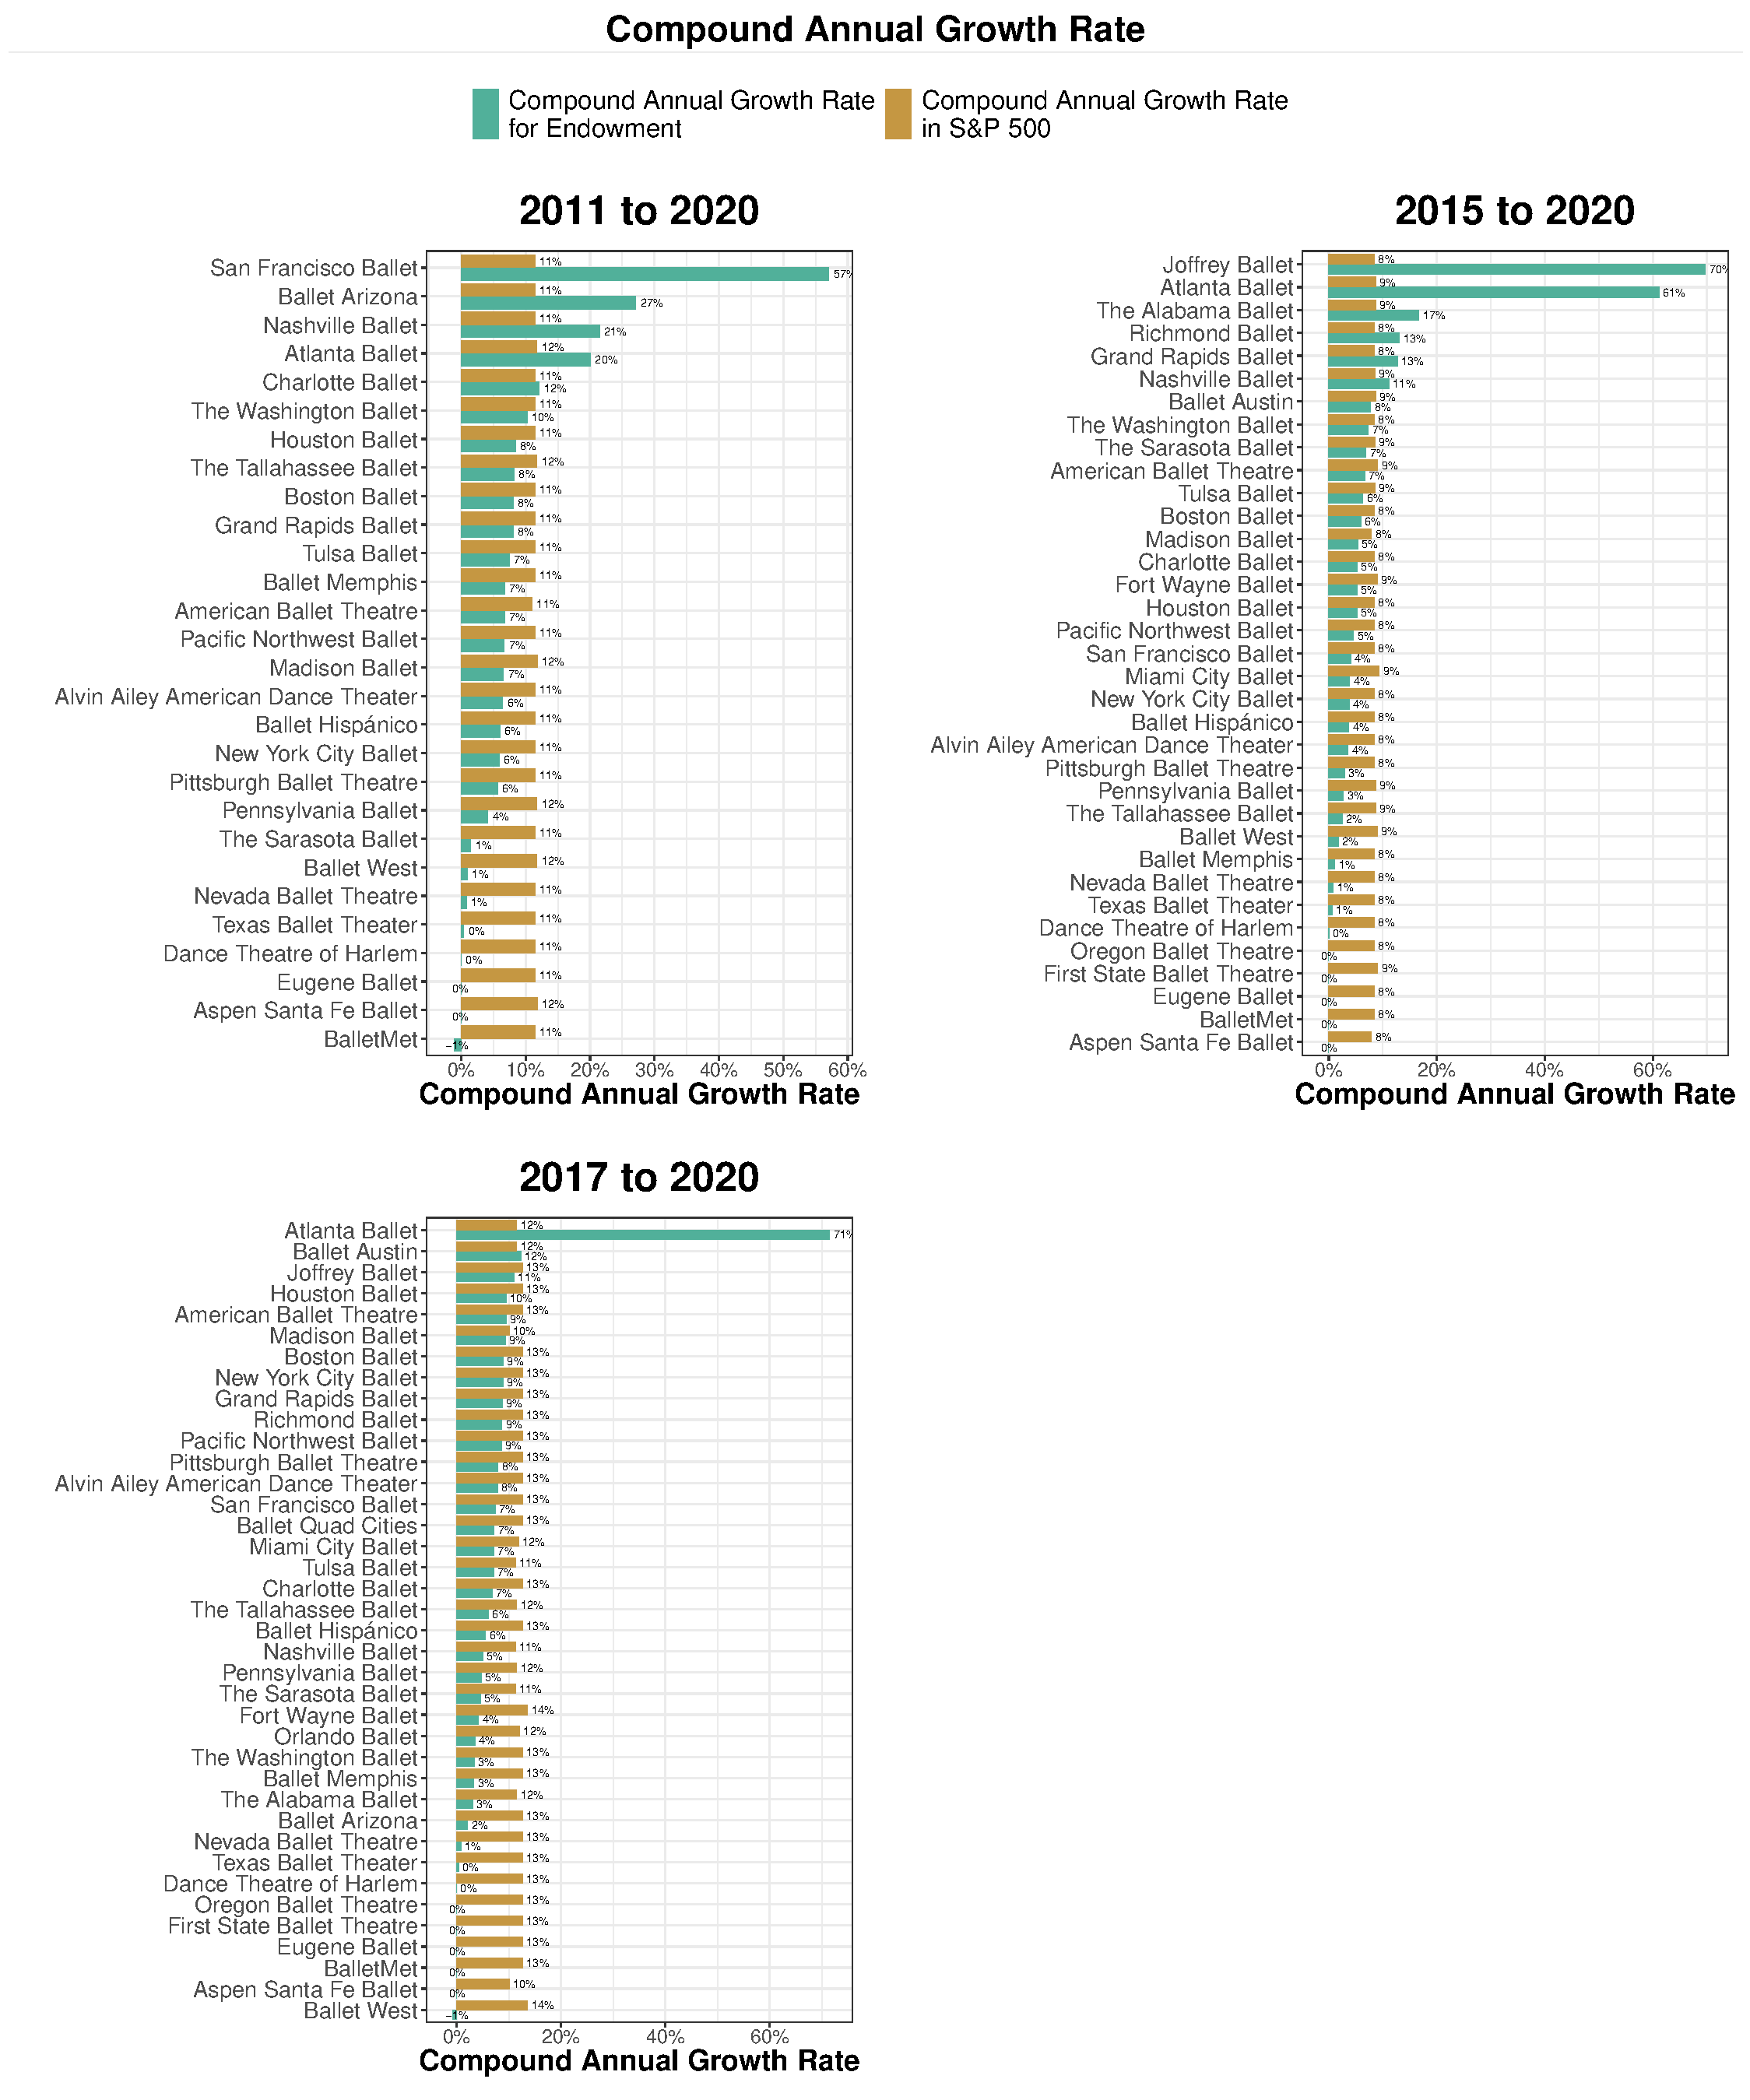
\includegraphics[width=0.9\linewidth,]{../images/compound-growth} \caption{\label{fig:compound-growth} Compound annual growth rates for all organizations compared to the compound annual growth rate for the S\&P 500 for three time periods. Not all companies are present in each plot since not all companies have data going back the same number of years. Of note, year-to-year differences in the compound annual growth rate of the S\&P 500 are due to differences in companies' fiscal years.}\label{fig:unnamed-chunk-12}
\end{figure}

\begin{figure}[H]
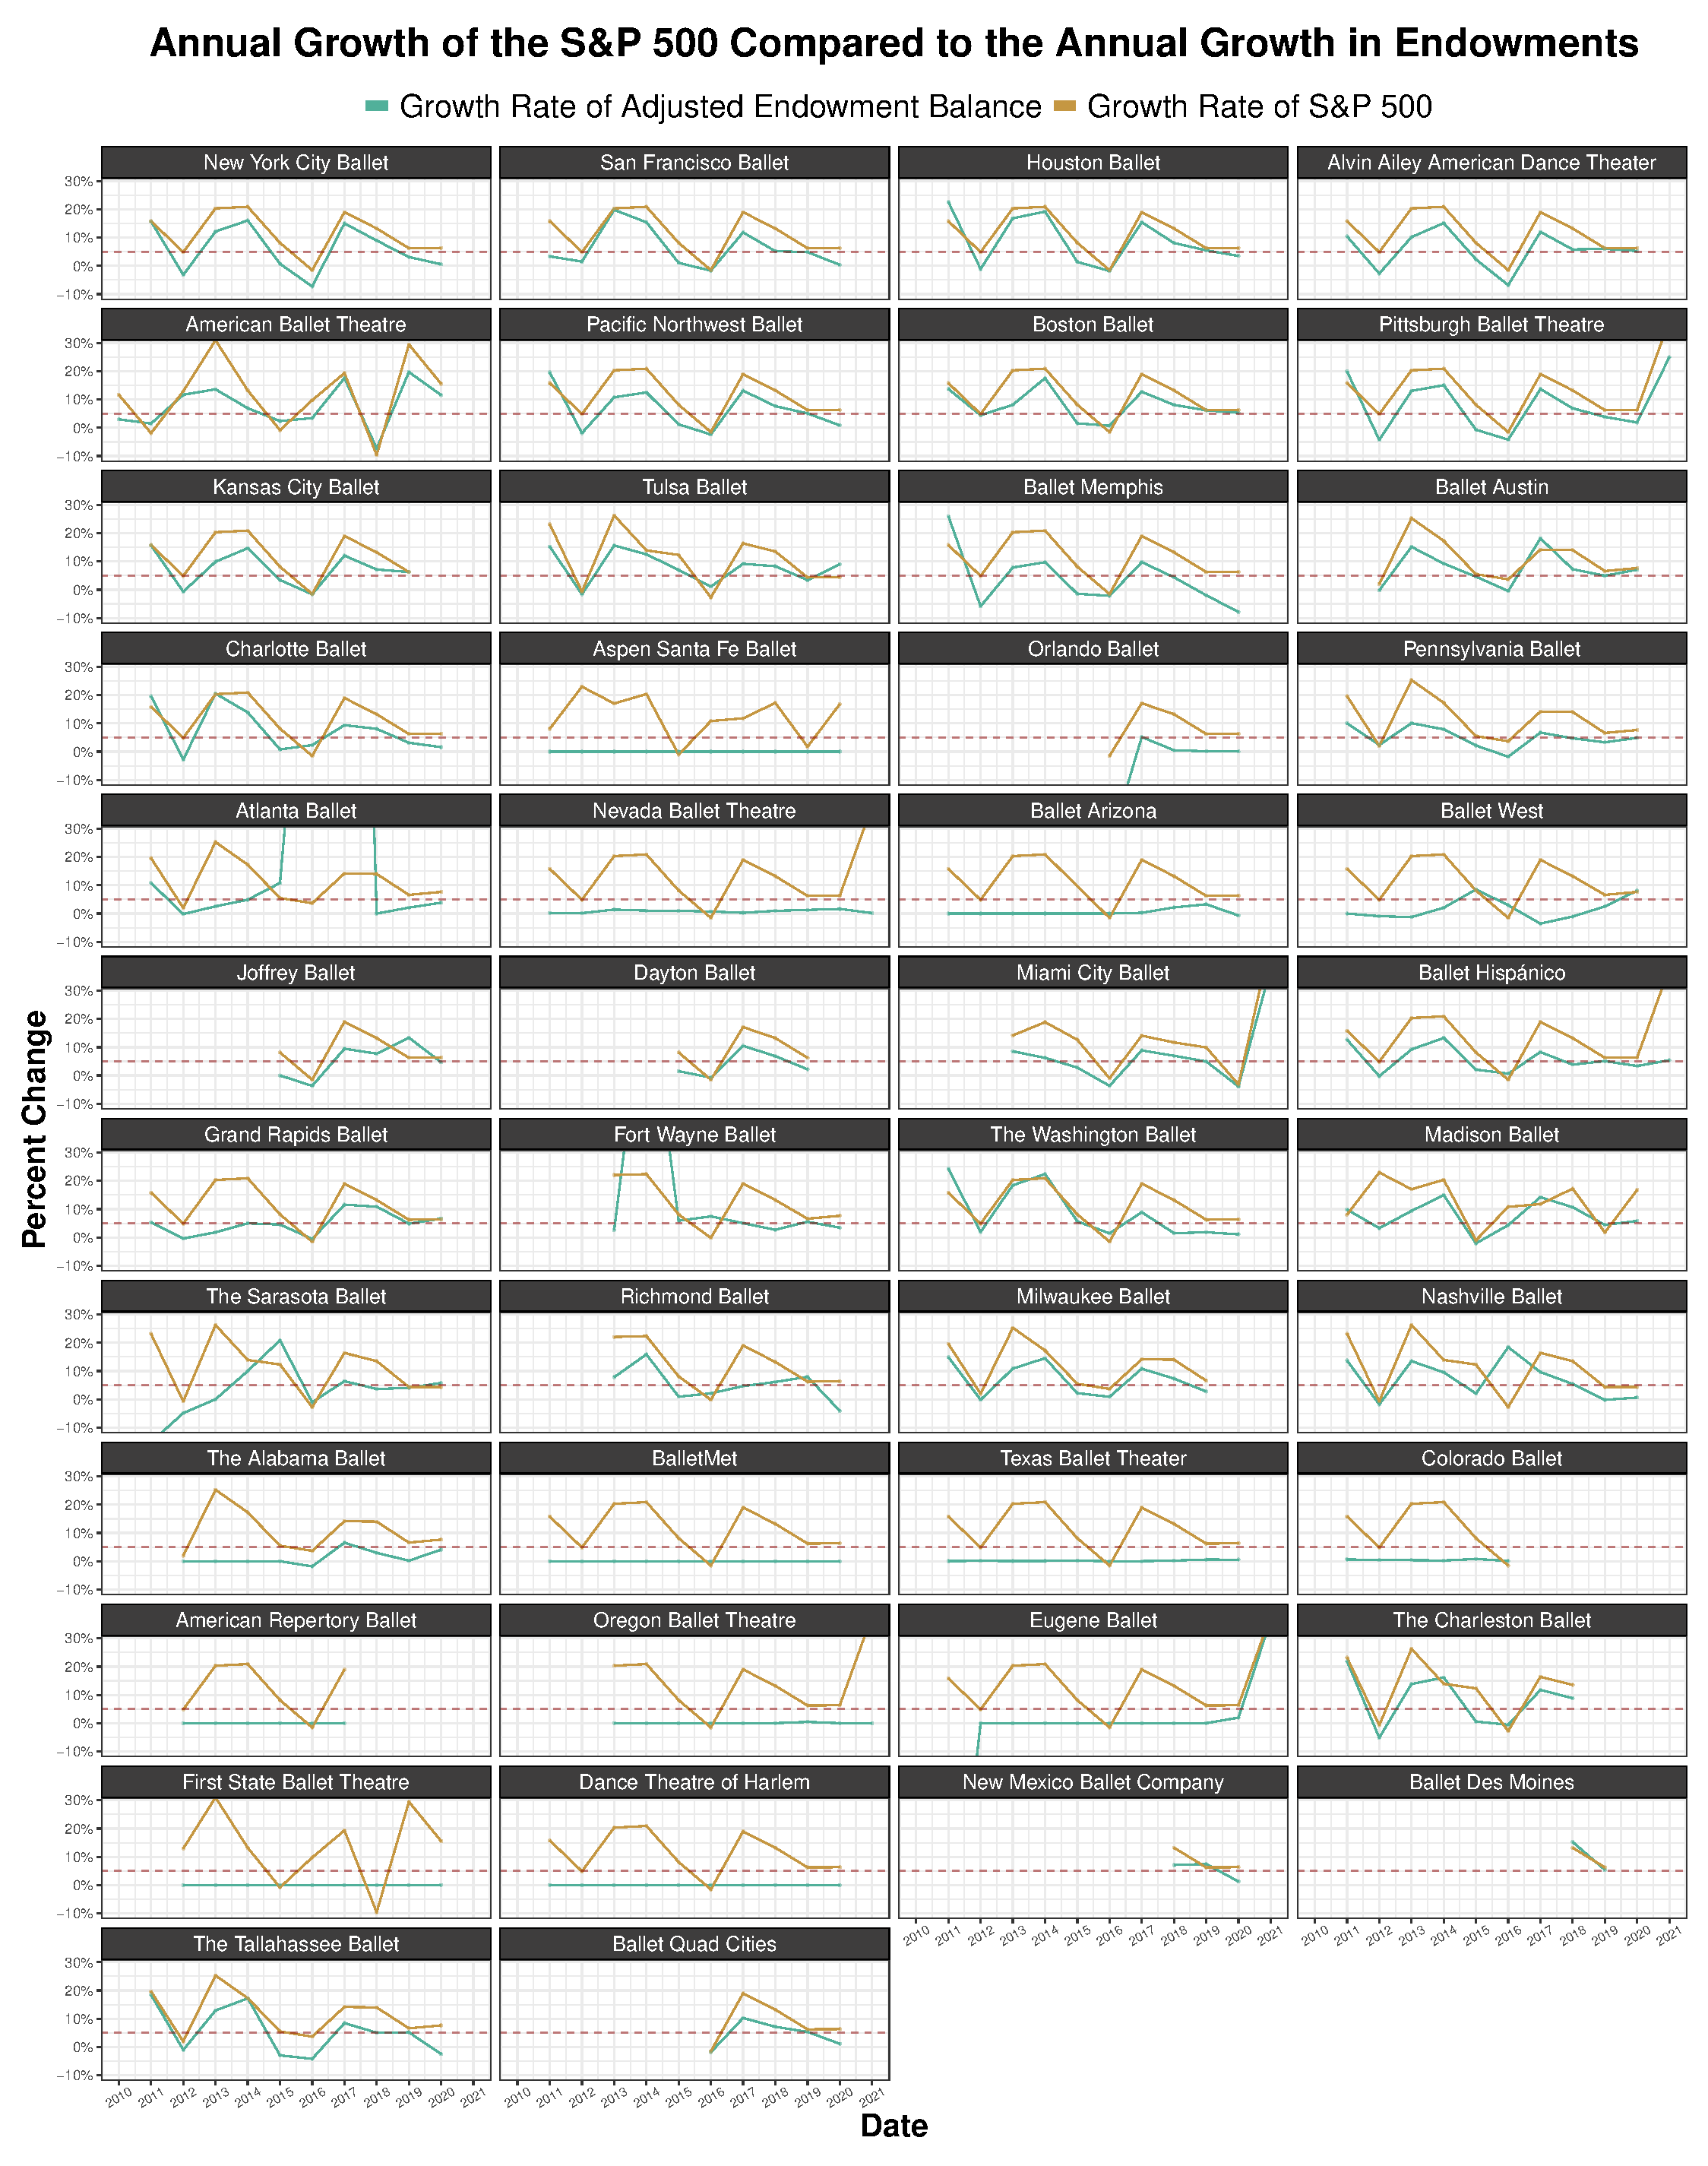
\includegraphics[width=0.9\linewidth,]{../images/annual-growth} \caption{\label{fig:annual-growth-endowment} Annual growth rate of a company's endowment when adjusting for contributions and withdrawals, compared to the annual growth S\&P 500 for the corresponding time period. Companies are ordered by mean endowment size across years on file, with companies with the largest endowments appearing first. A horizontal line at 5 percent is shown for reference.}\label{fig:unnamed-chunk-13}
\end{figure}

\newpage

\hypertarget{volunteer-paid-labor}{%
\subsection{Volunteer \& Paid Labor}\label{volunteer-paid-labor}}

\hypertarget{key-takeaways-1}{%
\subsubsection{Key Takeaways}\label{key-takeaways-1}}

\begin{itemize}
\tightlist
\item
  The highest proportion of companies who rely more on volunteer labor
  than paid employees is the South, then the Midwest, followed by the
  West, then Mid-America, New England, and then the Mid-Atlantic.\\
\item
  The percent paid to C-Suite employees ranges from 0\% to a little over
  30\%, and consistently has a median near 10\% (Figure
  \ref{fig:frac-comp}). Companies with notable changes in the percent
  paid to C-Suite employees across years includes First State Ballet
  Theatre, American Repertory Ballet, Cincinnati Ballet, and Oregon
  Ballet Theatre (Figures \ref{fig:frac-comp} and
  \ref{fig:csuite-comp-bar})
\end{itemize}

\hypertarget{volunteer-labor-and-geography}{%
\subsubsection{Volunteer Labor and
Geography}\label{volunteer-labor-and-geography}}

Overall, more labor (both volunteer and employee) is used in the West,
followed by the Mid-Atlantic, then the South, then the Midwest, then
Mid-America, and finally New England. Of these regions, the one with the
highest proportion of companies who rely more on volunteer labor than
paid employees is the South, then the Midwest, followed by the West,
then Mid-America, New England, and then the Mid-Atlantic.

In Figure \ref{fig:type-region-bar}, the South has the most companies
who use more volunteers than employees with 68\% of all reported
companies volunteers, followed by the Midwest, then the West, then
Mid-America, New England, and finally the Mid-Atlantic.

\begin{figure}[H]
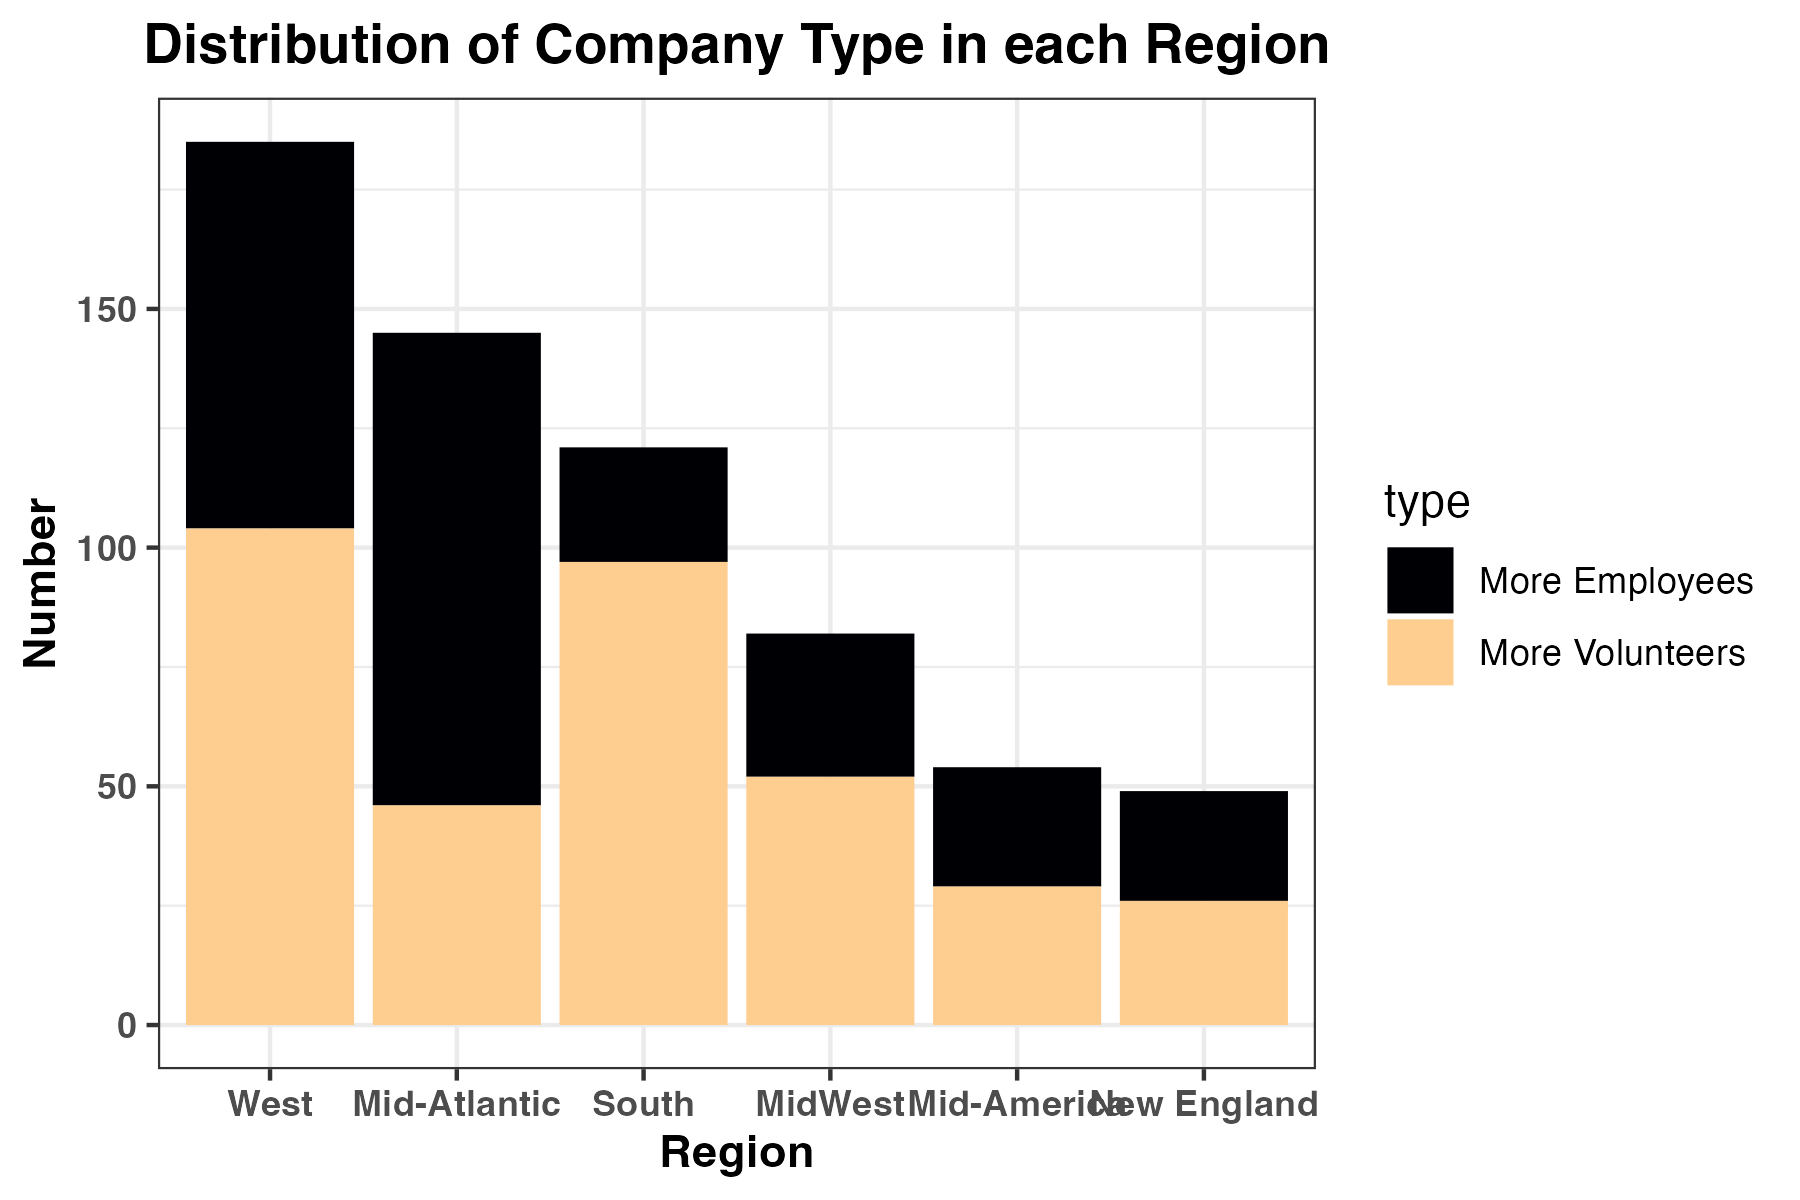
\includegraphics[width=0.9\linewidth,]{../images/type_region_bar} \caption{\label{fig:type-region-bar}Total number of laborers reported for each region in the 2019 fiscal year, colored by the number of companies who report either more employees or more volunteers}\label{fig:unnamed-chunk-14}
\end{figure}

Figure \ref{fig:ratio-region} shows the 1st, 2nd, 3rd, and 4th quantiles
of total volunteer labor. Individual companies were ranked by the total
number of volunteers they reported and then computed the quantiles. The
share within each quantile is shown by region.

\begin{figure}[H]
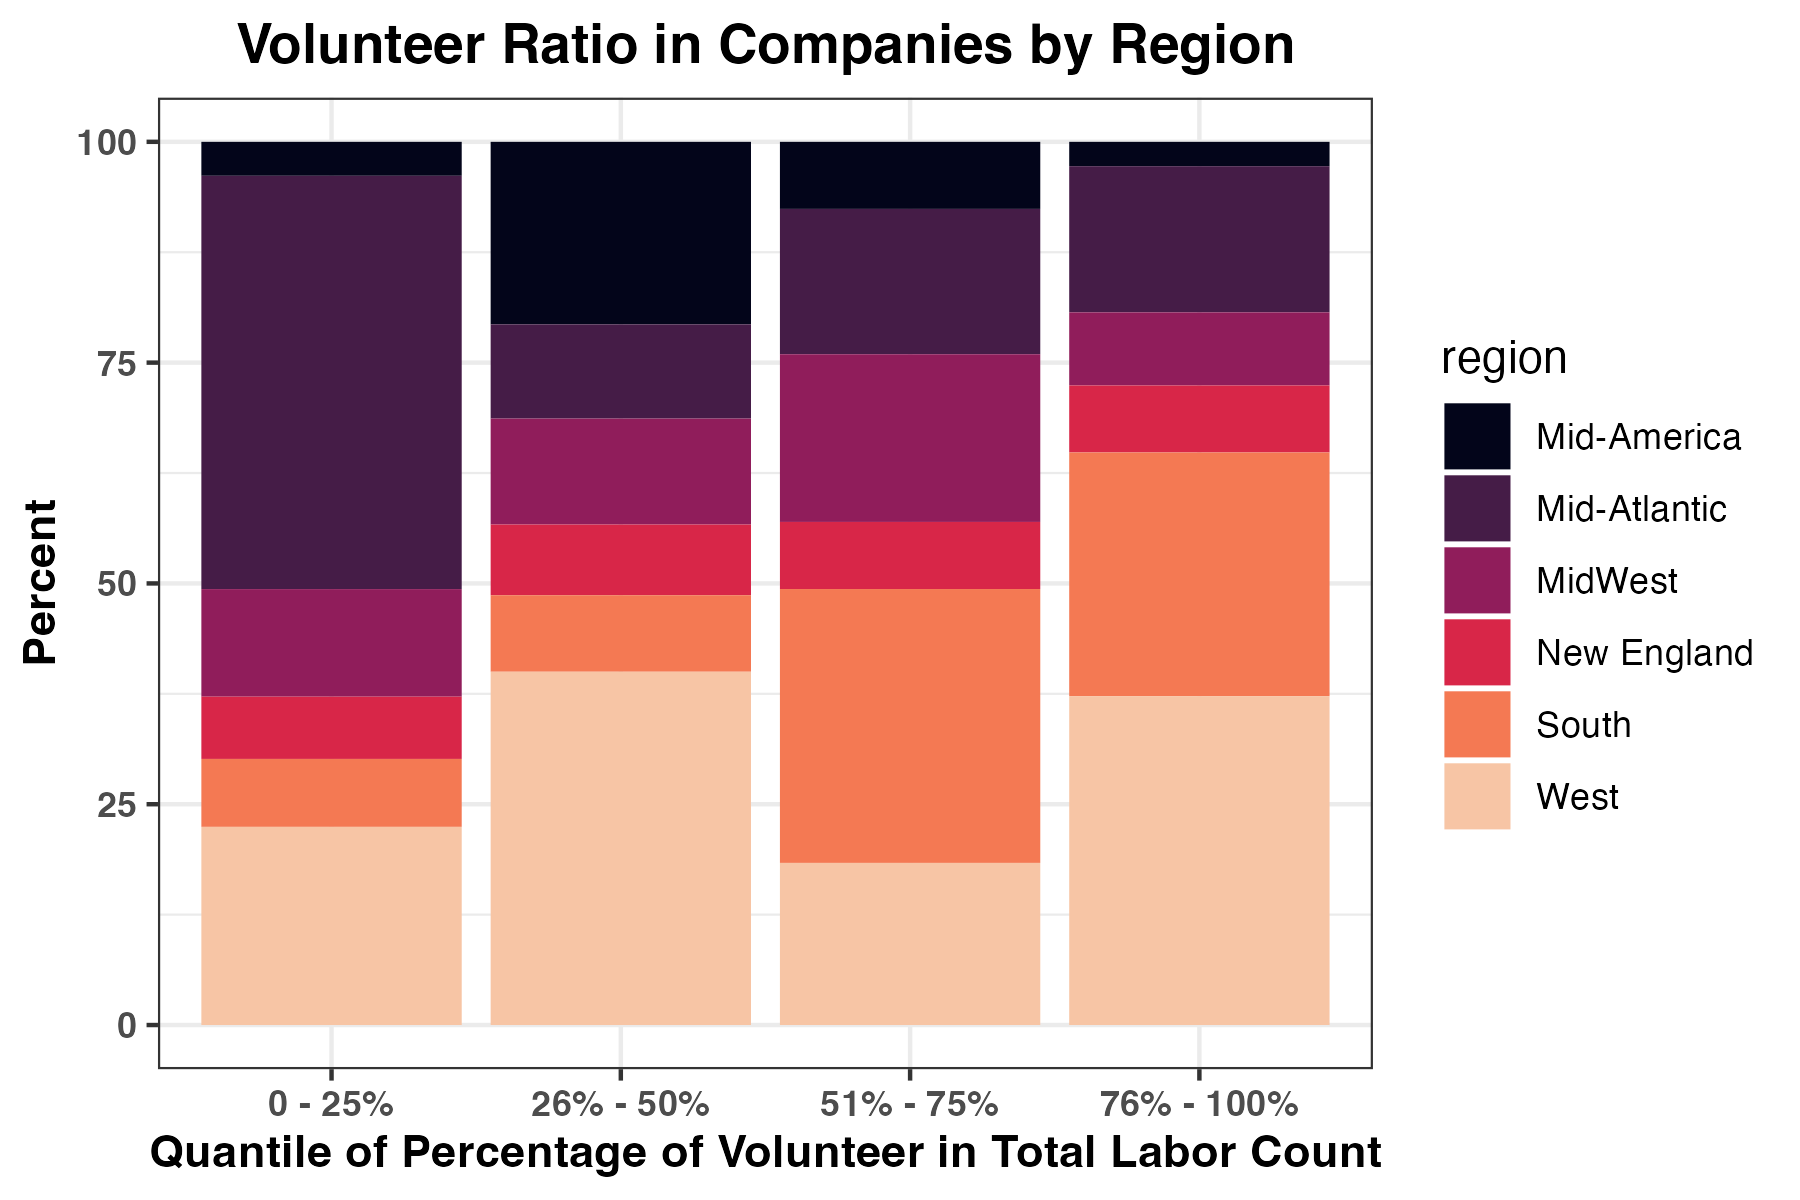
\includegraphics[width=0.9\linewidth,]{../images/ratio_bar_region} \caption{\label{fig:ratio-region}Share of volunteer use for each region by quantile using individual companies.}\label{fig:unnamed-chunk-15}
\end{figure}

We visualize the percentage of total labor that was volunteer labor by
state across the United States in Figure \ref{fig:us-map}.

\begin{figure}[H]
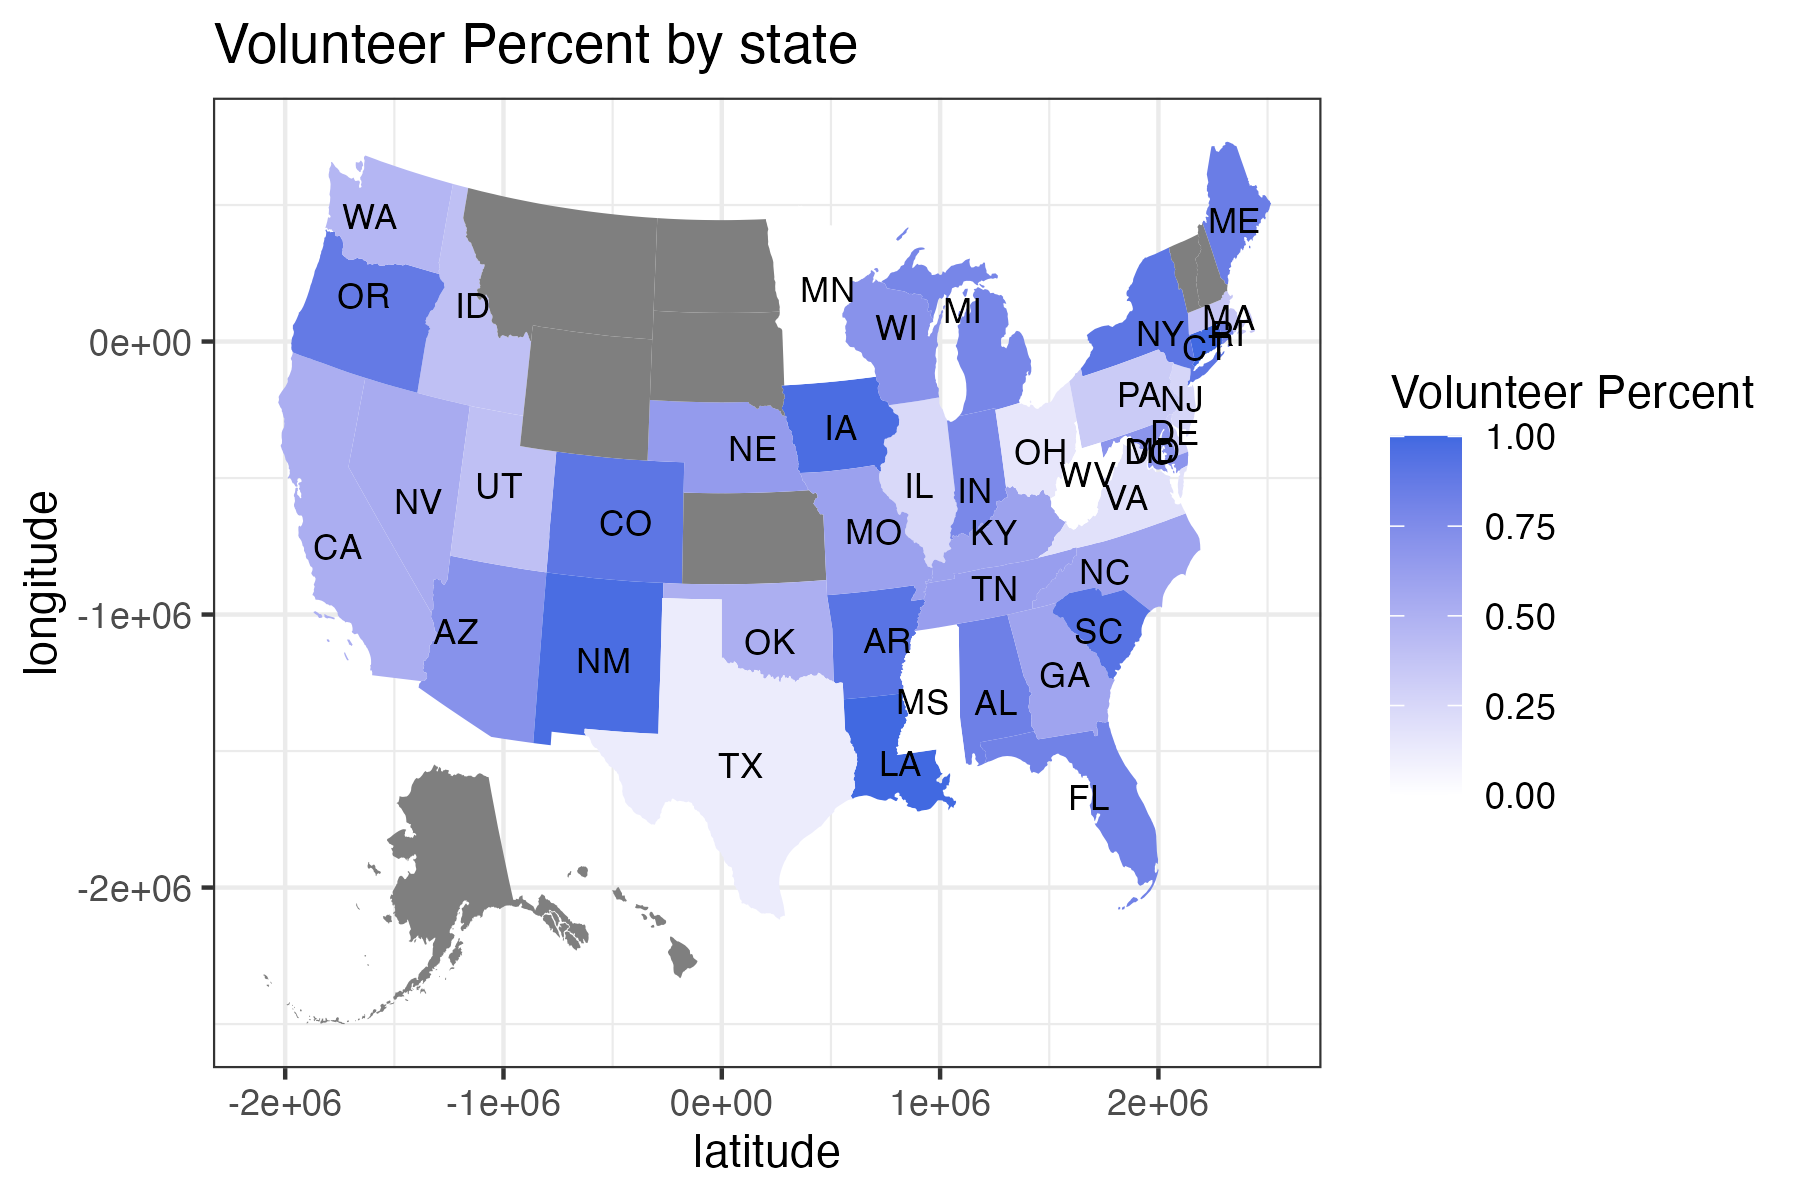
\includegraphics[width=0.9\linewidth,]{../images/vol_map} \caption{\label{fig:us-map}Share of volunteer labor among all labor by state. States, which do not have data, are in gray.}\label{fig:unnamed-chunk-16}
\end{figure}

\newpage 

\hypertarget{compensation-to-top-employees}{%
\subsubsection{Compensation to Top
Employees}\label{compensation-to-top-employees}}

While thinking about paid and unpaid labor in the dance industry, it is
also useful to look at how compensation is distributed among paid
employees.

In Part IX of Form 990, companies report compensation going to the set
of top employees -- in particular, ``officers, directors, trustees, and
key employees''; this set of top employees is referred to as C-Suite
employees. Additionally, they report the total compensation to all
employees.

This information allows for a comparison of what percent of total
employee compensation was going to C-Suite employees. For this analysis,
only companies with more than 45 employees were included. This choice
was due to the extent of variability in the percentages paid to C-Suite
employees in companies smaller than this threshold size since there are
some years where smaller companies report zero compensation to C-Suite
employees.

Of note, Aspen Santa Fe Ballet has previously contacted DDP® regarding
C-Suite compensation, as they amended their fiscal year 2020 990s;
however, as the IRS is behind in its uploading of amended returns, the
corrected information is not publicly available.

The percentage paid to C-Suite employees ranges from 0\% to a little
over 30\%, and is fairly constant over the years (Figure
\ref{fig:frac-comp} ). The median for each fiscal year was close to
10\%. However, the limited data available for 2021 shows that
percentages appear to increase following the onset of the pandemic; this
trend will be important to consider as more data from 2021 is released.

In Figure \ref{fig:csuite-comp-bar}, where the difference in the
percentage of total compensation paid to C-Suite employees in 2020 to
that in 2015 is summarized, there's actually a fairly even split between
companies that increased the percent paid to C-Suite employees versus
those that decreased the percent going to C-Suite employees.

\begin{figure}[H]
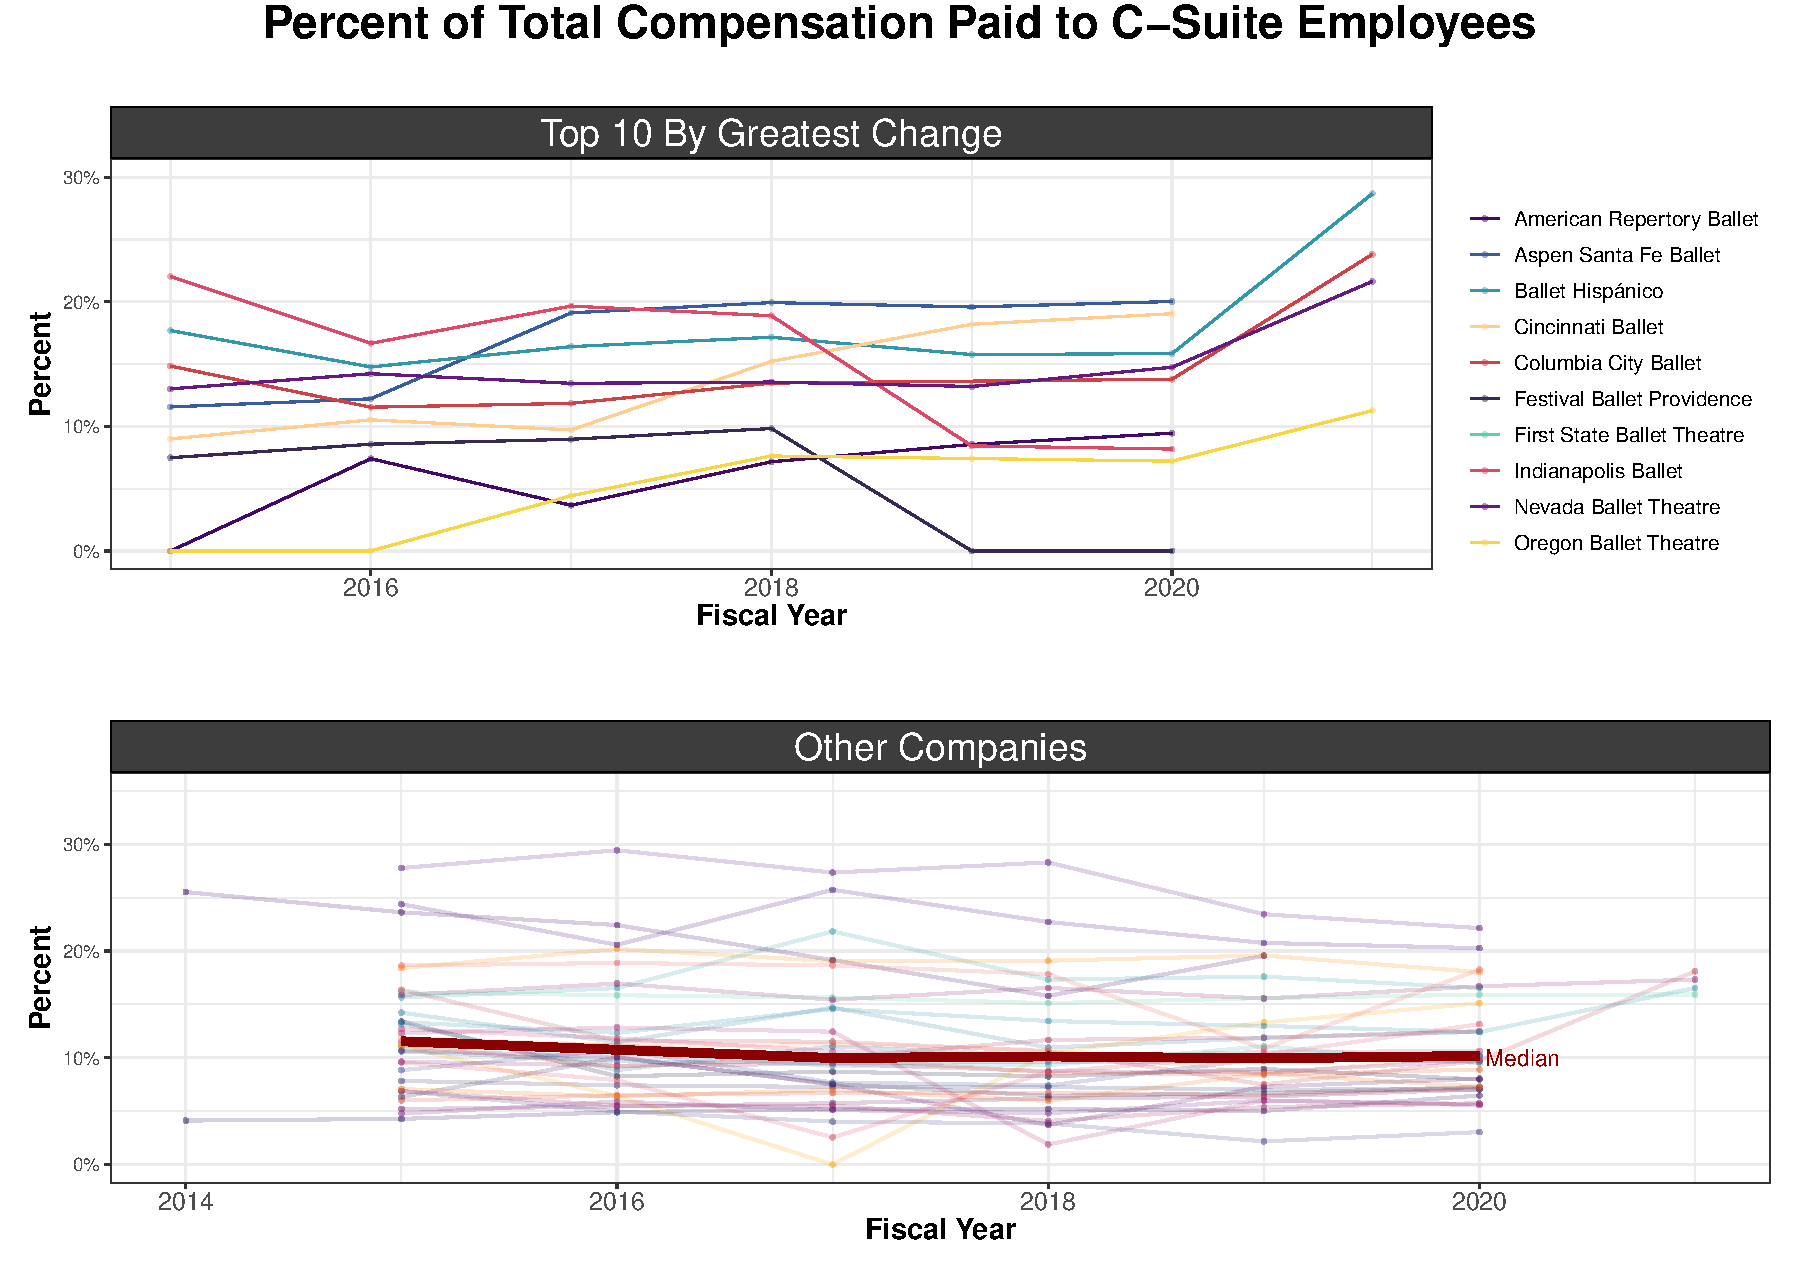
\includegraphics[width=0.9\linewidth,]{../images/frac-comp} \caption{\label{fig:frac-comp} Percent of the total compensation paid to employees that were paid to officers, directors, trustees, or key employees, as reported in Part IX of Form 990. Highlighted in the first panel are the 10 companies that had the greatest change in the percent paid to C-Suite employees from the earliest year on file to the latest. Only companies with more than 45 employees and that reported complete data for more than 5 years are included.}\label{fig:unnamed-chunk-17}
\end{figure}

\begin{figure}[H]
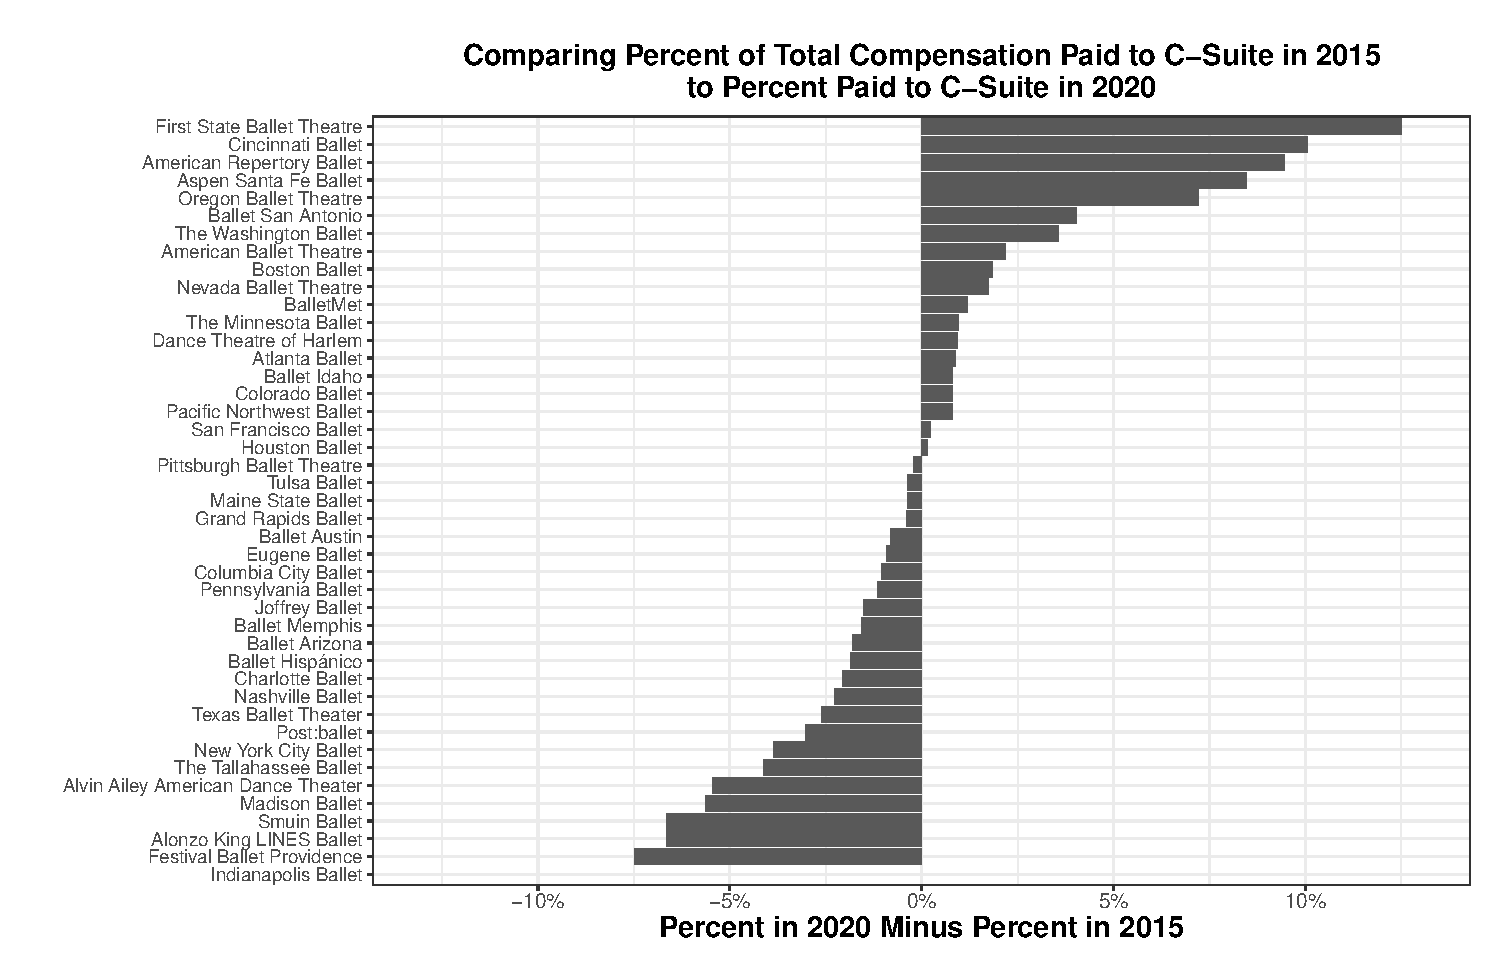
\includegraphics[width=0.9\linewidth,]{../images/csuite-comp-bar} \caption{\label{fig:csuite-comp-bar} Comparing the percent of total compensation paid to C-Suite employees in 2015 to that in 2020. Since the 2015 percent were subtracted from the 2020 percent, positive values indicate a greater percentage of compensation went to C-Suite employees in 2020, while negative values indicate a smaller percentage of compensation went to C-Suite employees in 2020.}\label{fig:unnamed-chunk-18}
\end{figure}

\hypertarget{buildings}{%
\subsection{Buildings}\label{buildings}}

\hypertarget{key-takeaways-2}{%
\subsubsection{Key Takeaways}\label{key-takeaways-2}}

\begin{itemize}
\tightlist
\item
  Most companies have stable building endowments except those that went
  through major buying or saving behaviors.\\
\item
  For those companies that went through major changes in buying or
  selling behaviors in buildings and lands, no specific patterns as
  found in years or regions.\\
\item
  The state that has the most companies might not have the highest sum
  of buildings book values, which indicates that different states have
  different niches for dance companies.
\end{itemize}

In-person performances are a huge part of dance companies' business, and
many shows are held in companies' theaters. Therefore, analyzing how
each company's endowment of buildings and lands, especially their book
values, is important in understanding how these companies are faring
economically.

In this analysis, book values were defined as the value of the asset
recorded on the balance sheet, as reported in Part VI of Schedule D of
Form 990. For all the analyses included below, the book values are
summed from all the buildings and lands owned by the company.

In the following plots, we split the companies into groups (high,
medium, and low) based on their book values to visualize companies that
had book values in a similar range. This makes trends more clear because
companies' book values are on such different scales, with some companies
approaching \(8 \times 10^7\) in book values, while others had less than
\(1 \times 10^5\). Companies were divided into these three groups based
on the quantile of their building's book value in 2020.

\hypertarget{trends-in-property-book-values-highmediumlow-by-quantile}{%
\subsubsection{Trends in Property Book Values (high/medium/low by
quantile)}\label{trends-in-property-book-values-highmediumlow-by-quantile}}

\begin{figure}[H]
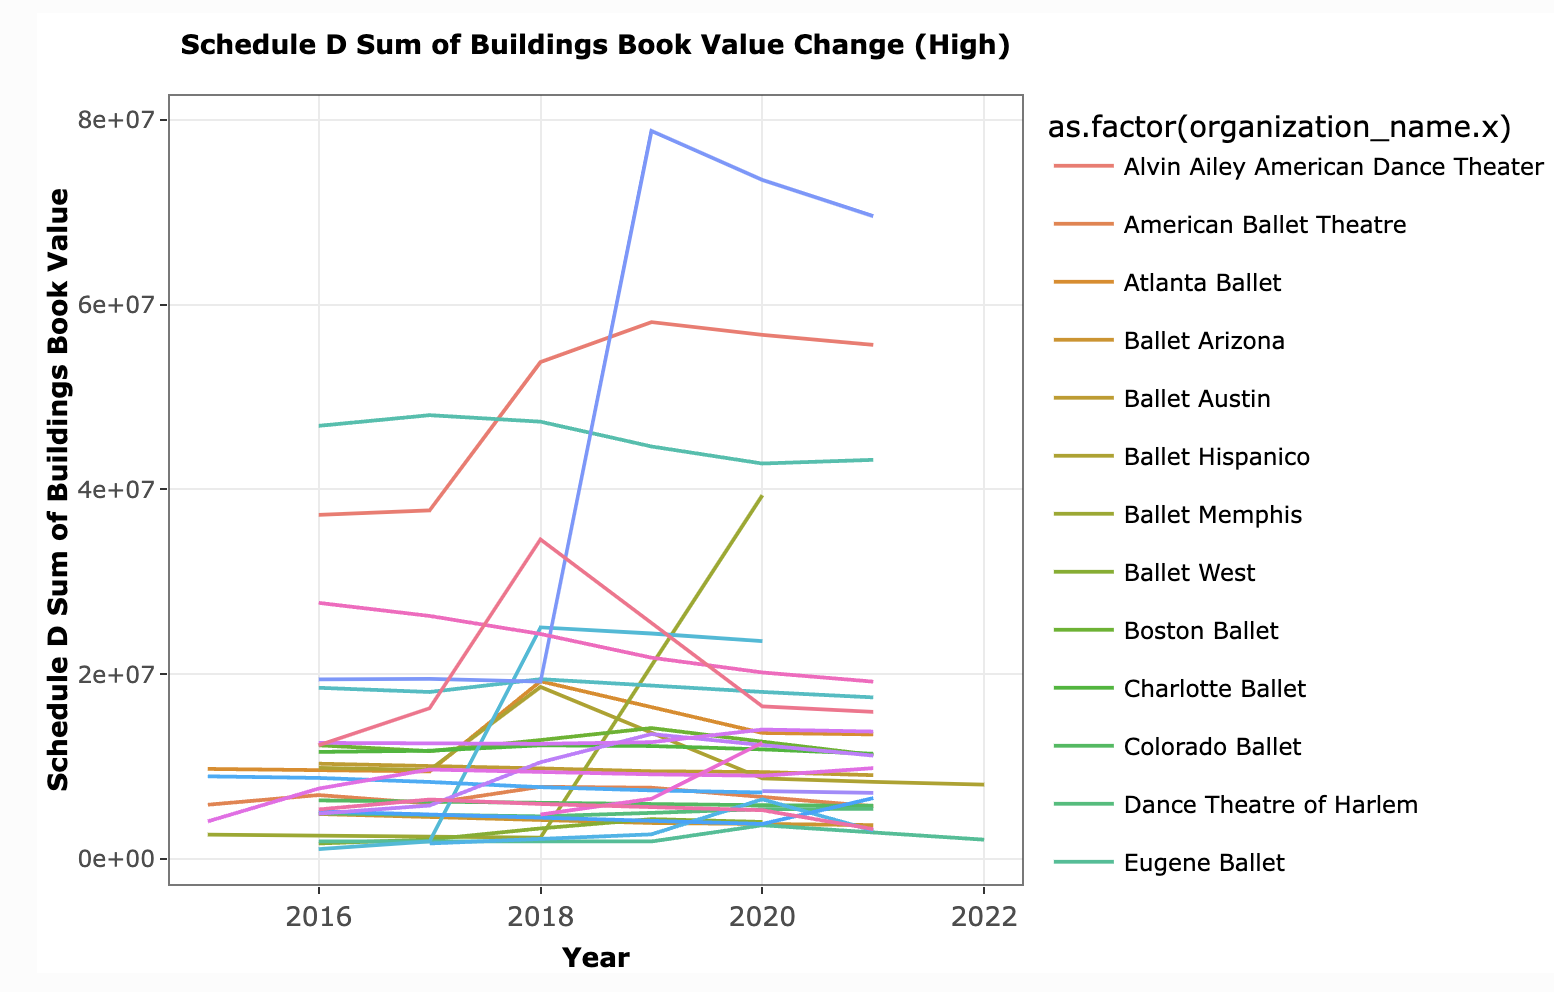
\includegraphics[width=0.8\linewidth,]{../images/high} \caption{\label{fig:high}}\label{fig:unnamed-chunk-19}
\end{figure}

\begin{figure}[H]
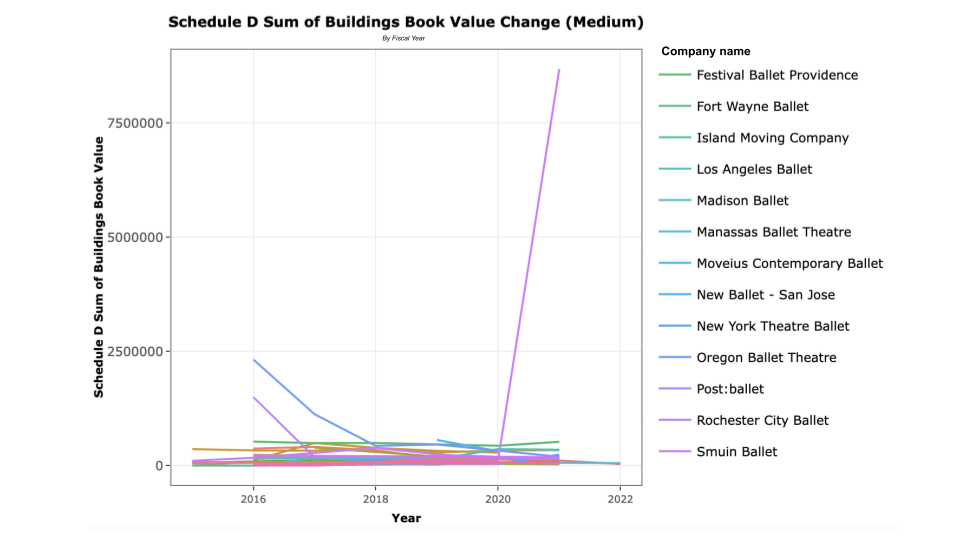
\includegraphics[width=0.8\linewidth,]{../images/medium} \caption{\label{fig:medium}}\label{fig:unnamed-chunk-20}
\end{figure}

\begin{figure}[H]
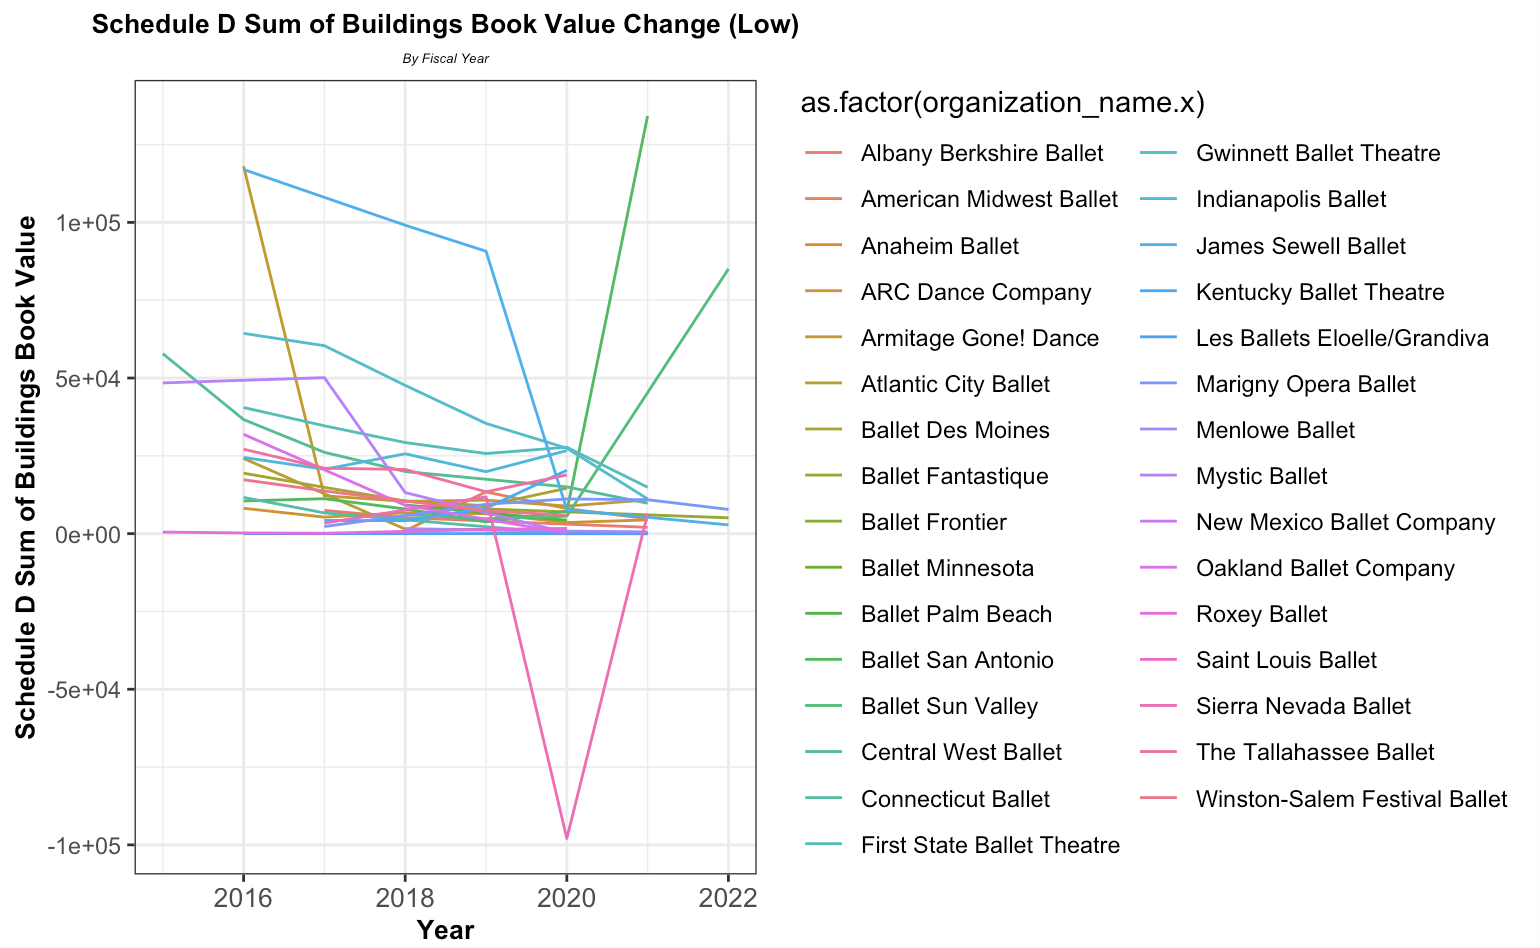
\includegraphics[width=0.8\linewidth,]{../images/low} \caption{\label{fig:low}}\label{fig:unnamed-chunk-21}
\end{figure}

In Figures \ref{fig:high}, \ref{fig:medium}, and \ref{fig:low}, the
percent changes in buildings' book values for each company from 2014 to
2021 are presented. Companies with notable changes for each category
are:

\begin{itemize}
\tightlist
\item
  Major: New York City Ballet, Ballet Memphis, Tulsa Ballet.\\
\item
  Medium: Smuin Ballet\\
\item
  Low: Saint Louis Ballet, Les Ballets Eloelle/Grandiva, Ballet Palm
  Beach
\end{itemize}

\hypertarget{percent-change-in-building-book-values}{%
\subsubsection{Percent change in Building Book
Values}\label{percent-change-in-building-book-values}}

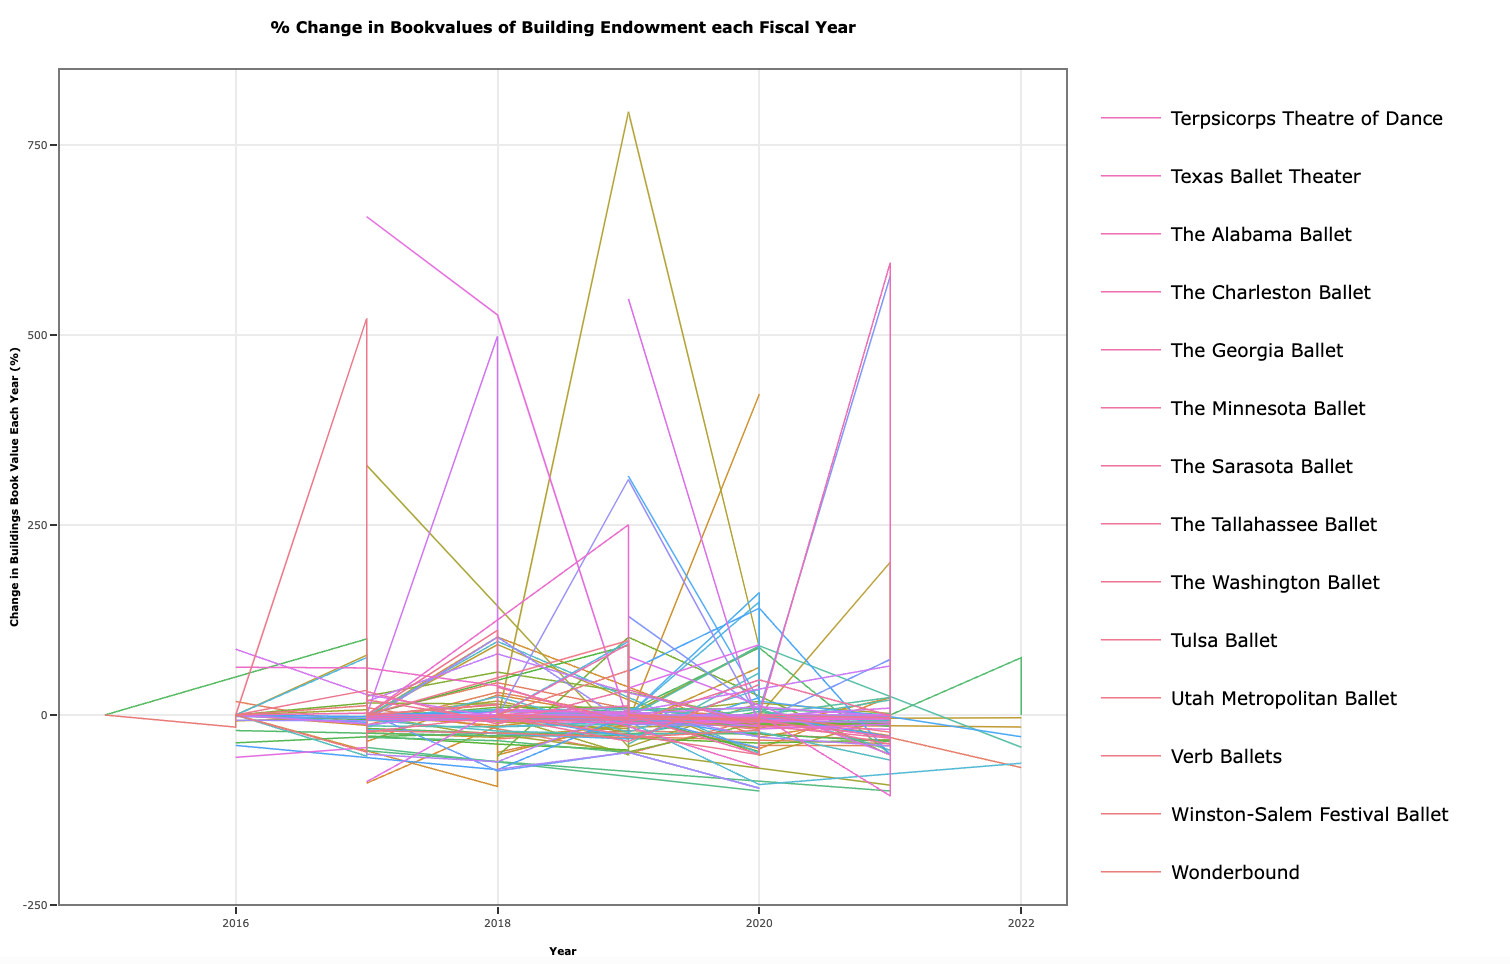
\includegraphics[width=0.9\linewidth,]{../images/percentage_building}

Most companies have decreased building book values over time except
those companies that went through major changes in selling and buying
buildings. The companies went through larger changes including Utah
Metropolitan Ballet, Post:Ballet, Ballet Memphis, Philadanco, New Ballet
San Jose, Sacramento Ballet, Marigny Opera Ballet, and Ballet Idaho.

\hypertarget{percent-change-in-ranking}{%
\subsubsection{Percent Change in
Ranking}\label{percent-change-in-ranking}}

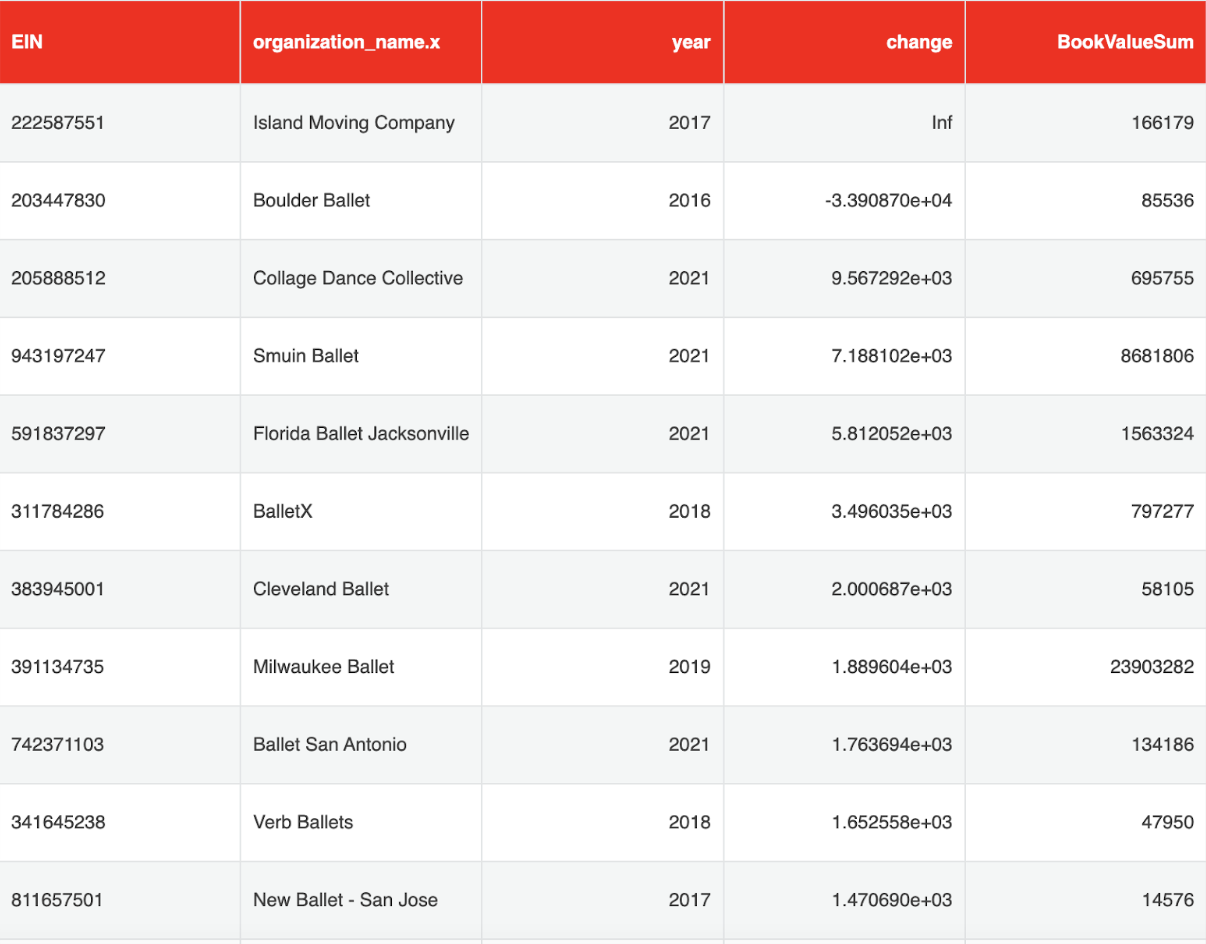
\includegraphics[width=0.6\linewidth,]{../images/percent_change_ranking}

\hypertarget{percentage-change-in-book-value-by-year}{%
\subsubsection{Percentage change in book value by
year}\label{percentage-change-in-book-value-by-year}}

We can see from the mean that many extreme values exist in terms of
changes in the building's book values.

\hypertarget{conclusions}{%
\section{Conclusions}\label{conclusions}}

\hypertarget{data-quality}{%
\subsection{Data Quality}\label{data-quality}}

As stated in the introduction, online reporting of tax returns by dance
companies has facilitated this research; however, a long-standing issue
with publicly-available tax reporting is there is no guarantee that
mistakes are not made and published. Therefore, a significant part of
our analyses was focused on checking the quality, completeness, and
aberrations in values reported on the 990 forms. Many discrepancies were
found indicating non-concordance concerning the end-of-year balances and
beginning-of-year balances within the same year for many companies,
where the values reported don't match indicating missing information.
Additionally, values reported for previous years did not match what
certain companies actually filed for those years with no apparent
explanation. Many companies the capstone team reached out to for
clarification did not respond. This issue should be addressed in future
analyses. Implications for missing or inaccurate reporting on Form 990s
and 990EZs include misinforming the public. Data analyses run on
inaccurate information may also draw false conclusions about the
financial practices of certain companies that don't really exist.
Informing dance companies of the importance of proper tax reporting may
help address these errors in the future.

\hypertarget{endowments-and-the-sp-500}{%
\subsection{Endowments and the S\&P
500}\label{endowments-and-the-sp-500}}

Our analyses have demonstrated that the trends of the stock market, and
particularly the S\&P 500, heavily influence percent change in the
endowments of many companies. Other companies perform very differently
from the S\&P 500. This indicates that companies significantly differ in
their investment behavior. Some companies differ in their investment
behavior. Some companies, such as Oregon Ballet Theatre and Aspen Santa
Fe Ballet\footnote{Recall the note on Aspen Santa Fe Ballet mentioned
  \hyperref[sec:asfb]{earlier}.}, did not invest their endowments at
all. Others, including San Francisco Ballet, Arizona Ballet, Joffrey
Ballet, and Houston Ballet, saw substantial investment gains over the
years that were analyzed. This has significant implications for the
individual dancers employed by these companies in terms of compensation
opportunities as well as job security. A company that does not earn
investment income risks long-term operation deficits due to inflation
and unforeseen expenses. Therefore, it is important to continue to
examine changes in endowments for dance companies over time and clearly
communicate these findings to the dance world.

\hypertarget{employee-and-volunteer-labor}{%
\subsection{Employee and Volunteer
Labor}\label{employee-and-volunteer-labor}}

\hypertarget{by-geographical-region}{%
\subsubsection{By Geographical Region}\label{by-geographical-region}}

The most volunteer labor is used in the South, followed by the Midwest,
followed by the West, then Mid-America, New England, and then the
Mid-Atlantic. There are several possible explanations for trends in
labor usage that are beyond the scope of what can be analyzed with Form
990 data. This indicates that a few things could be happening in the
world of dance. First, in regions with high rates of volunteer labor,
there may be a higher percentage of community engagement. This is
especially true for companies such as Eugene Dance in Oregon from the
West region, which reports a significant number of volunteers but
generates significant community support for their productions. Secondly,
in regions with high rates of employee labor, state, and local
governments may subsidize compensation costs which increase companies'
ability to hire and pay their employees. Since dance is known to be an
industry with a disproportionate amount of unpaid labor, it is
especially important to understand where and why these discrepancies
occur.

\hypertarget{compensation}{%
\subsection{Compensation}\label{compensation}}

The fraction of compensation going to senior executives (i.e.~their
C-Suite employees) is generally consistent, with a median of close to
10\% across all years on file. Future research should track trends of
executive compensation throughout the pandemic since the (limited) data
available showed the fraction going to C-Suite employees increased from
2020 to 2021.

\hypertarget{building-values}{%
\subsection{Building Values}\label{building-values}}

Additionally, the pattern of how dance companies use their building
endowment is inconsistent. Further investigation is required to fully
understand why and how real estate is used by these companies.

The wide-ranging impacts of these understandings may lead to greater
awareness by unpaid and underpaid laborers in dance, accountability for
dance companies, and more equity in the dance industry. The capstone
team hopes this work motivates further investigation of dance companies'
publicly available 990 data to better understand the financial
performance and decisions of dance companies, as well as other companies
in the performing arts.

\hypertarget{limitations}{%
\section{Limitations}\label{limitations}}

Our analyses were not without limitations. First, certain companies have
discrepancies in their End-of-Year and Beginning-of-Year balances.
End-of-Year balances were used to calculate the percent change in
endowments of all dance companies, so some information may be
misrepresented based on these discrepancies. Additionally, data on a
finer time scale, for example at the monthly time scale rather than the
yearly, would be more informative for studying how investments did over
time; however, 990 Forms only provide this data annually. Another
limitation of this work is the analysis of compensation. The Form 990
provides summarized information across total employees, along with some
information about compensation to C-Suite executives. However, it is not
directly clear from this data which of these employees are dancers, and
as such, it is not clear how dancers are being compensated relative to
other employees. Finally, a significant number of companies did not
report their number of employees and/or their number of volunteers. This
led to missing data that was left out of the geographical and unpaid
labor analyses. Nine states (New Hampshire, Vermont, Kansas, Wyoming,
South Dakota, North Dakota, Montana, Hawaii, and Alaska) did not have
any companies in this analysis.

\hypertarget{future-research}{%
\section{Future Research}\label{future-research}}

Because the IRS is
\href{https://www.propublica.org/article/irs-hasnt-released-nearly-half-million-nonprofit-tax-records}{behind
on releasing Form 990s}, only data from a smaller subset of companies
exists for 2021, which includes 29 companies in total. That said, the
effect of the COVID-19 pandemic on all trends examined here is a crucial
area of future research. Because the federal government issued billions
of dollars in public subsidies, trends throughout the pandemic would be
helpful to identify whether these subsidies helped those intended.
Similarly, it would be interesting to see if the COVID-19 pandemic has
changed the way companies used and reported their building endowment
found in this study, Lockdown policies in each state might change how
in-person performances were held, and companies might shut down certain
performance centers due to prolonged quarantine. Therefore, future
research on buildings' book values should be conducted after more data
in 2021 and 2022 is uploaded. Yet, to date, no comprehensive analysis
has been done on the wage gap in dance throughout the pandemic. Once tax
documents through 2022 are filed for these companies, future research
can examine how wages, income, operations, and unpaid labor at dance
companies have evolved throughout the pandemic.

\hypertarget{not-to-be-published-what-weve-learned-and-suggested-capstone-future-steps}{%
\section{NOT TO BE PUBLISHED: What We've Learned and Suggested Capstone
Future
Steps}\label{not-to-be-published-what-weve-learned-and-suggested-capstone-future-steps}}

\hypertarget{discrepancies}{%
\subsection{Discrepancies}\label{discrepancies}}

\begin{itemize}
\tightlist
\item
  Reporting of endowment values across years in Schedule D is not always
  consistent. Correspondence from companies the capstone team has heard
  from so far has indicated that the most recently reported values are
  correct, so the analyses were structured to take the most recent data
  available rather than the current-year reported value to be true.
\item
  A limit of our current understanding of reporting endowment data is
  what companies mean when they report negatives. In particular, are
  negatives in the expenses erroneous, or do they indicate something
  meaningful? In some cases, taking the expenses to be positive makes
  the calculated end-of-year balance concordant with the reported
  end-of-year balance, but in other cases taking the expenses to be
  positive causes a discrepancy to arise. These nuances will be
  important to future analyses of Form 990 data, so clarifying what
  companies mean when they report negative values in expenses in
  Schedule D is a useful area for future work.
\item
  Preparing emails to companies with these discrepancies is important,
  but very time-consuming, so allocating enough time if this needs to be
  done is advised. It took our team several days of labor to put
  together emails.\\
\item
  It might be worth asking companies who skip reporting 990s in certain
  years why they do so because there were some gaps in filings.
\end{itemize}

\hypertarget{endowments-over-time}{%
\subsection{Endowments Over Time}\label{endowments-over-time}}

\begin{itemize}
\tightlist
\item
  Information can be best analyzed and assessed using comparable
  measurements, e.g.~rankings and percent change, as endowment totals
  are widely varied between companies.\\
\item
  Further, in plots that contain main different companies over time, it
  is difficult to tell the difference between companies. Plots in the
  future should contain either separate tables with a color key,
  highlighted outliers, or other means of communicating which line
  refers to which company.\\
\item
  Endowments can be transferred between different entities (e.g.~Aspen
  Santa Fe Ballet). It would be worth checking this for more companies,
  and figuring out the best way to examine the exact transfer of
  funds.\\
\item
  In the future, examining various metrics in finance for evaluating
  investment behavior, e.g., Sharpe's Ratio, or average performance, may
  provide a more comprehensive understanding of companies' investment
  decisions.\\
\item
  More broadly, questions regarding the beginning of an endowment
  warrant further attention. In particular, at what point does a company
  typically create an endowment? Is that based on the size of the budget
  and years in business?
\end{itemize}

\hypertarget{unpaid-labor}{%
\subsection{Unpaid Labor}\label{unpaid-labor}}

\begin{itemize}
\tightlist
\item
  Geographical region is very important when considering how much
  volunteer labor is used.\\
\item
  It may also be interesting to analyze the companies with the largest
  endowments or net revenue and how much they use volunteer labor.\\
\item
  It is unknown how the breakdown of the types of volunteers they have:
  those volunteers could be dancers, or other individuals engaging in
  the various kinds of work needed to keep a dance company going.
\end{itemize}

\hypertarget{building-value-analyses}{%
\subsection{Building Value Analyses}\label{building-value-analyses}}

\begin{itemize}
\tightlist
\item
  There is a substantial amount of variability in the trends in building
  book values over time. Future work may evaluate specific companies
  with large changes and incorporate outside information on what
  decisions these changes correspond to (for example, if there is a
  purchase of a specific building for the company reported on their
  website or a news source).\\
\item
  It may also be interesting to study the relationship between changes
  in building book values and a company's endowment size, revenue, or
  other variables reported in Form 990.
\end{itemize}

\hypertarget{compensation-1}{%
\subsection{Compensation}\label{compensation-1}}

\begin{itemize}
\tightlist
\item
  Studying the relationship between the gender and pay of C-suite
  employees throughout the pandemic \emph{and} by geographical region
  might be an interesting step once the 2021 990s are published.
  However, this would require outside data, since gender is not reported
  on Form 990s.\\
\item
  It may also be interesting to look at how much employees are paid in
  various companies and regions (not just C-suite ones).
\end{itemize}

\hypertarget{pandemic}{%
\subsection{Pandemic}\label{pandemic}}

\begin{itemize}
\tightlist
\item
  Once the IRS releases filings for fiscal years 2020, 2021, and 2022,
  looking into how the trends presented here to change over the pandemic
  year will be informative for understanding how dance companies fared
  financially throughout the pandemic and the choices they made to
  navigate this tumultuous period.\\
\item
  When studying the impact of the pandemic, fiscal year \emph{end date},
  not just \emph{end year}, should be utilized for time series analyses,
  as a company whose 2020 fiscal year ends in March will have gone
  through very different events within their fiscal year as a company
  whose 2020 fiscal year ends in September.\\
\item
  Incorporating state-level COVID-19 policy information (e.g.,
  restrictions on large gatherings, or restaurant closures) may provide
  insight into how companies fared during the pandemic across locations.
  This would affect companies' abilities to rehearse or perform
  throughout the pandemic.
\item
  Understanding how endowments and trends in volunteer/paid labor will
  be crucial for understanding how the pandemic impacted dance
  companies.
\end{itemize}

\hypertarget{relating-endowment-work-to-ddps-other-analyses}{%
\subsection{Relating Endowment Work to DDP's Other
Analyses}\label{relating-endowment-work-to-ddps-other-analyses}}

\begin{itemize}
\tightlist
\item
  Our work here focused strictly on Form 990 data, but DDP® has covered
  a collection of other topics on these dance companies. Relating
  metrics related to gender equity to compensation or endowment trends
  may be an interesting avenue for future exploration.\\
\item
  For example, it would be interesting to examine the relationships
  between:

  \begin{itemize}
  \tightlist
  \item
    Endowment size and gender equity index
  \item
    Unpaid labor utilization and gender equity index.
  \end{itemize}
\end{itemize}

% %%%%%%%%%%%%%%%%%%%%%%%%%%%%%%%%%%%%%%%%%%
% %% optional
% \supplementary{The following are available online at www.mdpi.com/link, Figure S1: title, Table S1: title, Video S1: title.}
%
% % Only for the journal Methods and Protocols:
% % If you wish to submit a video article, please do so with any other supplementary material.
% % \supplementary{The following are available at www.mdpi.com/link: Figure S1: title, Table S1: title, Video S1: title. A supporting video article is available at doi: link.}

\vspace{6pt}

%%%%%%%%%%%%%%%%%%%%%%%%%%%%%%%%%%%%%%%%%%
\acknowledgments{The authors thank the support and mentorship of
Dr.~Lindsay Poirier, Andrew Hoekstra, and Elizabeth Yntema.}

%%%%%%%%%%%%%%%%%%%%%%%%%%%%%%%%%%%%%%%%%%

%%%%%%%%%%%%%%%%%%%%%%%%%%%%%%%%%%%%%%%%%%
\conflictsofinterest{The authors declare no conflict of interest.}

%%%%%%%%%%%%%%%%%%%%%%%%%%%%%%%%%%%%%%%%%%
%% optional
\abbreviations{The following abbreviations are used in this manuscript:\\

\noindent
\begin{tabular}{@{}ll}
DDP® & Dance Data Project \\
IRS & Internal Revenue Service \\
\end{tabular}}


%%%%%%%%%%%%%%%%%%%%%%%%%%%%%%%%%%%%%%%%%%
% Citations and References in Supplementary files are permitted provided that they also appear in the reference list here.

%=====================================
% References, variant A: internal bibliography
%=====================================
%\reftitle{References}
%\begin{thebibliography}{999}
% Reference 1
%\bibitem[Author1(year)]{ref-journal}
%Author1, T. The title of the cited article. {\em Journal Abbreviation} {\bf 2008}, {\em 10}, 142--149.
% Reference 2
%\bibitem[Author2(year)]{ref-book}
%Author2, L. The title of the cited contribution. In {\em The Book Title}; Editor1, F., Editor2, A., Eds.; Publishing House: City, Country, 2007; pp. 32--58.
%\end{thebibliography}

% The following MDPI journals use author-date citation: Arts, Econometrics, Economies, Genealogy, Humanities, IJFS, JRFM, Laws, Religions, Risks, Social Sciences. For those journals, please follow the formatting guidelines on http://www.mdpi.com/authors/references
% To cite two works by the same author: \citeauthor{ref-journal-1a} (\citeyear{ref-journal-1a}, \citeyear{ref-journal-1b}). This produces: Whittaker (1967, 1975)
% To cite two works by the same author with specific pages: \citeauthor{ref-journal-3a} (\citeyear{ref-journal-3a}, p. 328; \citeyear{ref-journal-3b}, p.475). This produces: Wong (1999, p. 328; 2000, p. 475)

%=====================================
% References, variant B: external bibliography
%=====================================
\reftitle{References}
\externalbibliography{yes}
\bibliography{DDPCitations.bib}

%%%%%%%%%%%%%%%%%%%%%%%%%%%%%%%%%%%%%%%%%%
%% optional

%% for journal Sci
%\reviewreports{\\
%Reviewer 1 comments and authors’ response\\
%Reviewer 2 comments and authors’ response\\
%Reviewer 3 comments and authors’ response
%}

%%%%%%%%%%%%%%%%%%%%%%%%%%%%%%%%%%%%%%%%%%


\end{document}
